\documentclass[a4paper,12pt]{article}
\usepackage{color}
\usepackage[usenames,dvipsnames,svgnames,table]{xcolor}
\usepackage{listings}
\usepackage[T1]{fontenc}
\usepackage{imakeidx}
\usepackage{graphicx}
%\makeindex[columns=3, title=Alphabetical Index, intoc]
\usepackage{graphicx,wrapfig,lipsum}

\usepackage[hmargin=1cm, vmargin=3cm]{geometry}
\usepackage[font=tiny, labelfont=sc]{caption}
\usepackage{hyperref}

%\usepackage{refcount}


%hyperlinks, coloured menu, submenu with different colors, clickable references
\hypersetup{
     colorlinks   = true,
     citecolor    = gray
}

\usepackage{tocloft}

\renewcommand{\cftsubsecfont}{\normalfont\hypersetup{linkcolor=cyan}}
\renewcommand{\cftsubsecafterpnum}{\hypersetup{linkcolor=green}}

\newcommand{\wrapfill}{\par\ifnum\value{WF@wrappedlines}>0
  \addtocounter{WF@wrappedlines}{-1}%
  \null\vspace{\arabic{WF@wrappedlines}\baselineskip}%
  \WFclear
\fi}


\author{
  Daniele, Della Cioppa\\
  \texttt{daniele.dellacioppa@gmail.com}
}
\title{Usage of the \texttt{\textbackslash author} command}

\renewcommand{\footnotesize}{\scriptsize}


%for chinese characters - not working yet
\usepackage{CJKutf8}
\usepackage[utf8]{inputenc} % optional
\usepackage[T1]{fontenc}


% for underlining
\usepackage{ulem}


%\usepackage{fontspec}

%\newfontfamily{\cfont}{Microsoft YaHei}


\begin{document}

\title{Networking}
\maketitle
\hypersetup{linkcolor=teal}
\tableofcontents
%\hypersetup{linkcolor=cyan}
%\listoffigures
\hypersetup{linkcolor=blue}
\clearpage

\part{The basics of Networks}


\begin{wrapfigure}[21]{5cm}
\centering
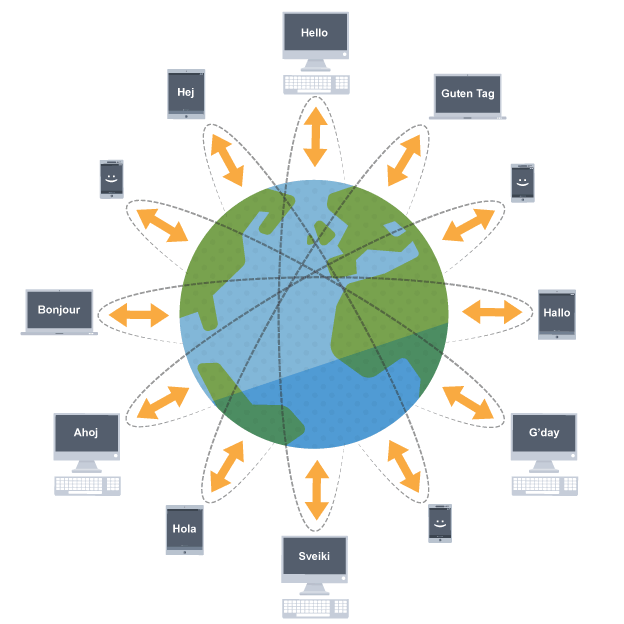
\includegraphics[width=12cm]{./net.png}
%\vspace{-10pt}
\caption{devices connected in the world}\label{wrap-fig:1}
\end{wrapfigure}

A network is two or more \emph{computers} (or other electronic devices) \textbf{connected} together, usually by cables(\textbf{guided}) or Wi-Fi(\textbf{unguided}).



\section {network benefits}
\begin{enumerate}
\item {sharing hardware, such as printers, computers, phones, tablets, scanners, etc...}\footnotemark{}
\item {sharing software, allowing:}
    \begin{itemize}
    \item{multiple users to run the same programs on different computers}
    \item{data to be shared, so that other people can access shared work}
    \item{you to access your data from any computer on the network}
    \end{itemize}
\end{enumerate}





\footnotetext{All these pieces of hardware are usually addressed as \textbf{endpoints} as long as they have the ability to communicate effectively within a network}


\newline \noindent Networking is crucial if you want to use your computer to communicate. Without it you couldn’t send an email, a text or an instant message and that would be so weird in 2022 isn't it?

\noindent We use a huge network on a daily basis and this is called the internet. Around three billion people use the internet to share data, news and resources, amongst many other things.
\clearpage
\subsection{guided wiring}
Is quicker than unguided, it consists in physical wires. Optic Fiber is on the top of this list but can't be twisted or the light will bounce back. You can install an optic cable for a much longer distance and you won't get the same troubles you would get with copper cables for example. But no twisting or it'll bounce back!

\subsection{unguided wiring}
The term \emph{wiring} can be deceiving here as there are literally no wires involved to realize the connection. In Cantonese is probably much clearer (Figure 2).


\begin{wrapfigure}{R}{11cm}
\centering
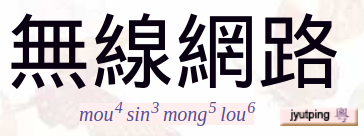
\includegraphics[width=5cm]{WiFi-HK.PNG}
%\vspace{-10pt}
\caption{Definition of WiFi in Historical Chinese commonly spoken in Hong Kong}\label{wrap-fig:5}
\end{wrapfigure}


Unguided wiring simply means Wi-Fi really. You can have a 2.4Ghz signal to reach longer distance but won't be nicely matched with a 5Ghz device. A 5Ghz device won't reach the same distance as a 2.4Ghz.Take a look how it's worded in Cantonese and you'll see a different etymological meaning from the English one\footnote{\label{wifialliance}stands for Wireless Fidelity.It kept this name for a short time after the brand name was created by the \href{https://en.wikipedia.org/wiki/Wi-Fi_Alliance}{Wi-Fi Alliance}.} but still both words suggest the idea that no wires are involved.


\wrapfill


\begin{wrapfigure}{L}{8cm}
\centering\newcommand{\wrapfill}{\par\ifnum\value{WF@wrappedlines}>0
  \addtocounter{WF@wrappedlines}{-1}%
  \null\vspace{\arabic{WF@wrappedlines}\baselineskip}%
  \WFclear
\fi}
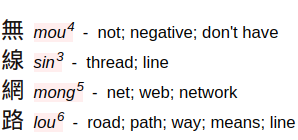
\includegraphics[width=8cm]{./WiFi-HK-details.PNG}
\vspace{-10pt}
\caption{Cantonese characters in the WiFi word}\label{wrap-fig:6}
\end{wrapfigure}


\noindent The first character represents the concept of \textbf{not} having ($mou^4$). The second one ($sin^3$) is literally thread or line so that's why \emph{wiring} to me is sort of misleading. 
If you ask a person :

\[Can\ you\ tell\ me\ what\ unguided\ wiring\ means?\]

\noindent Because of the word \emph{wiring} one could start thinking about a particular kind of special fancy wire. But wires are the last thing you'll ever see in the case of \textbf{unguided wiring}



%\begin{CJK}{UTF8}{gbsn}

%Without \texttt{CJKutf8} package, the result will be wrong.

%Café: 咖啡厅

%Gödel: 哥德尔

%© 版权所有

%無線網絡

%\end{CJK}

\section{LAN vs WAN}

LAN, which stands for \textbf{local area network}, and WAN, which stands for \textbf{wide area network}, are two types of networks and \texttt{\textit{as the naming conventions suggest}}, LANs are for more localized networking\footnote{\label{LAN}in a home,business,school,etc.}
\begin{wrapfigure}{R}{7cm}
\centering
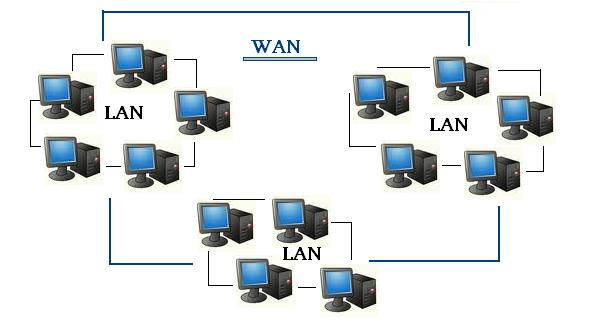
\includegraphics[width=5cm]{lan-wan.JPG}
%\vspace{-10pt}
\caption{difference between WAN and LAN}\label{wrap-fig:5}
\end{wrapfigure}

\noindent while WANs cover larger areas, such as cities, and even allow computers in different nations to connect.
LANs are typically faster and more secure than WANs, but WANs enable more widespread connectivity. Of course there are sort of exceptions like the NHS having a huge Local Area Network spread all over the country with local IP addresses starting in the first octet with \oldstylenums{10} instead of \oldstylenums{192}, thus using a Class A Address rather than a Class C (more on this topic in Chapter 33) 



\clearpage



\section{IEEE 802.3}

IEEE 802.3 is a set of standards and protocols that define Ethernet-based networks. Ethernet technologies
\begin{wrapfigure}[16]{1cm}
\centering
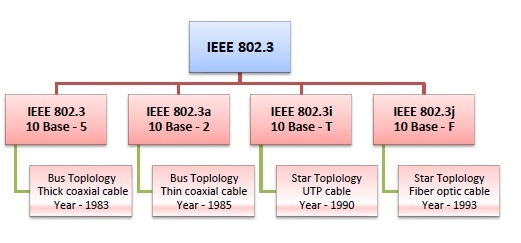
\includegraphics[width=13cm]{./ieee_802.jpg}
\vspace{-15pt}
\caption{IEEE cable hierarchy}\label{wrap-fig:2}
\end{wrapfigure}

\noindent are primarily used in LANs, though they can also be used in WANs as well.

IEEE 802.3 defines the physical layer and the medium access control (MAC) sub-layer of the data link layer for wired Ethernet networks. The unique identifier of our computer's motherboard is actually adhering to a standard defined by IEEE 802.3.
The psysical layer is the lowest layer identified in the TCP/IP protocol or the ISO/OSI protocol. The packets on the network before they finally go to destination they need to know which MAC address corresponds to the IP they hold already in the headers. In the next paragraph we'll explain the different cables in Figure 5.




\subsection{Popular Versions}

There are a number of versions of IEEE 802.3 protocol. The most popular ones are:



\begin{itemize}
\item{IEEE 802.3: This was the original standard given for coaxial (10BASE-5). Here, 10 is the maximum throughput which means 10 Mbps and 5 refers to the maximum segment length of 500m. If it goes longer than 500m there's no guarantee it'll work}
\item{IEEE 802.3a: This gave the standard for thin coax (10BASE-2), which is a thinner variety of coaxial cable. The 2 refers to the maximum segment length of about 200m (185m to be precise)}
\item{IEEE 802.3j: This gave the standard for Ethernet over Fiber (10BASE-F) that uses fiber optic cables as medium of transmission}
\end{itemize}

\clearpage

\section{Protocols}

Protocols are kind of rules defined in advance to make sure two or more devices know in advance what to expect if they send a particular message and what to expect in return 

\subsection{OSI Standard}
The Open Systems Interconnection (OSI) model describes seven layers that computer systems use to communicate over a network. It was the first standard model for network communications, adopted by all major computer and telecommunication companies in the early 1980s

\begin{wrapfigure}[21]{5cm}
\centering
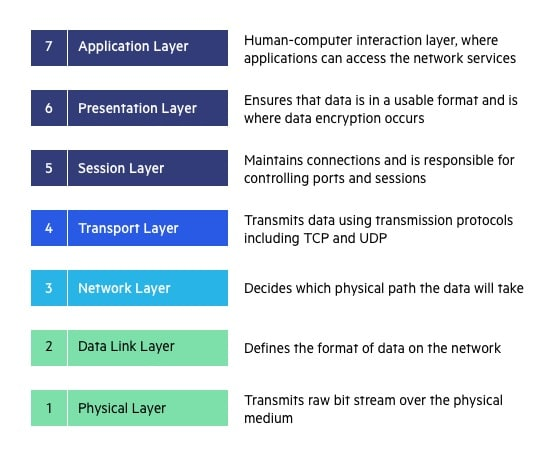
\includegraphics[width=12cm]{./OSI-7-layers.jpg}
%\vspace{-10pt}
\caption{OSI Layer representation}\label{wrap-fig:3}
\end{wrapfigure}


The modern Internet is not based on OSI, but on the simpler TCP/IP model. However, the OSI 7-layer model is still widely used, as it helps visualize and communicate how networks operate, and helps isolate and troubleshoot networking problems.


\subsection{A good Mnemonic}
One way to remember the OSI Layer is, as always, by using funny and silly stories but this time we won't be talking of italian clichés, mentioning videogames monsters or referencing Boris Johnson jumping from an airplane holding the British Flag (yes he did that as well) but we'll use this mnemonic insetead: 

\medskip
\noindent
\textsc{\textbf{P}lease \textbf{D}o \textbf{N}ot \textbf{T}hrow \textbf{S}ausage and \textbf{P}izza Away}}
\medskip

\noindent It's obtained by looking at the $1^{st}$ letter of each layer from the bottom

\subsection{Theory vs Practice}
Even if The Transmission Control Protocol/Internet Protocol (TCP/IP) model came before the Open Systems Interconnection (OSI) model it is what is used in practice today, and it has only five layers:

\begin{itemize}
\item {Application layer}
\item {Transport layer}
\item {Network access layer}
\item {Network interface layer}
\item {Hardware layer}
\end{itemize}

\noindent This may look drastically different from the OSI model, primarily because some functions are encompassed in a single layer: the application layer. In TCP/IP, this provides users with the physical standards, transport functions, network interface, and internetworking functions that correspond with the first three layers of the OSI model. In other words, in the TCP/IP model, these services are all done in the application layer.

TCP/IP is connection and connectionless

\subsection{horizontal vs vertical approach}
There's a debate on which one is vertical and which is horizontal so that point won't be discussed in this document for the time being.

\section{ARP/RARP/DHCP}
Address Resolution Protocol translates MAC addresses into IPs so that from the network layer we can communicate over the internet with IPs while RARP demands another computer (usually a server) to assign the demanding one with an IP which is essentially what DHCP is doing that's why RARP got obsolete
\subsection{ARP Tables}
These are used from every component in a network to know which MAC address the packet needs to point at 
On this machine for example all it needs to know is which is the MAC address of the gateway, and the TV who's connected in the same WiFi

\begin{lstlisting}
_gateway (192.168.0.1) at 24:a7:dc:31:5b:d1 [ether] on wlp3s0
TV (192.168.0.129) at cc:d3:c1:64:f9:f3 [ether] on wlp3s0
\end{lstlisting}

\subsection{Three-way-handshake}
This is when the client sends the ARP request to the server. The server does an aknowledgment and answers with an ARP reply saying both its MAC and its IP. It all happens like this :

When Computer 1 wants to talk to  Computer 2 in a local area network by Ethernet cables and network switches, with no intervening gateways or routers. Computer 1 has a packet to send to Computer 2. Through DNS, it determines that Computer 2 has the IP address 192.168.0.55.

To send the message, it also requires Computer 2's MAC address. First, Computer 1 uses a cached ARP table to look up 192.168.0.55 for any existing records of Computer 2's MAC address (00:EB:24:B2:05:AC). If the MAC address is found, it sends an Ethernet frame containing the IP packet onto the link with the destination address 00:EB:24:B2:05:AC. If the cache did not produce a result for 192.168.0.55, Computer 1 has to send a broadcast ARP request message (destination FF:FF:FF:FF:FF:FF MAC address), which is accepted by all computers on the local network, requesting an answer for 192.168.0.55.

Computer 2 responds with an ARP response message containing its MAC and IP addresses. As part of fielding the request, Computer 2 may insert an entry for Computer 1 into its ARP table for future use.

Computer 1 receives and caches the response information in its ARP table and can now send the packet

\clearpage

\section{Networking Hardware}
Computers need networking hardware in order to connect to each other. \textbf{Routers}, \textbf{hubs}, \textbf{switches} and \textbf{bridges} are all pieces of networking equipment that can perform slightly different tasks. A router can often incorporate hubs, switches and wireless access within the same hardware

\begin{wrapfigure}[18]{5cm}
\centering
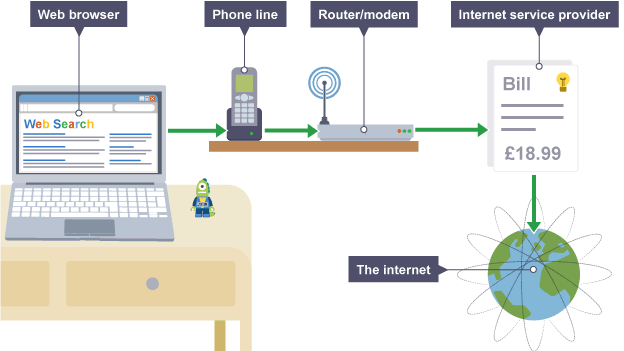
\includegraphics[width=16cm]{./large.PNG}
%\vspace{-10pt}
\caption{Router connecting devices in a LAN over the Internet}\label{wrap-fig:4}
\end{wrapfigure}

\subsection{Routers}
A router can form a \textbf{LAN} by connecting devices within a building. It also makes it possible to connect different networks together. Homes and businesses use a router to connect to the internet. A router can often incorporate a modem within the hardware.

\subsection{Modems}
A \textbf{modem} enables a computer to connect to the internet over a telephone line. A modem converts \textbf{digital} signals from a computer to analogue signals that are then sent down the telephone line. A modem on the other end converts the analogue signal back to a digital signal which another computer can understand.

\subsection{Hubs, bridges and switches}
\textbf{Hubs}, \textbf{bridges} and \textbf{switches} allow multiple devices to connect to the router and they transfer data to all devices on a network. A router is a more complex device that usually includes the capability of hubs, bridges and switches.

\clearpage

\begin{wrapfigure}{R}{11cm}
\centering
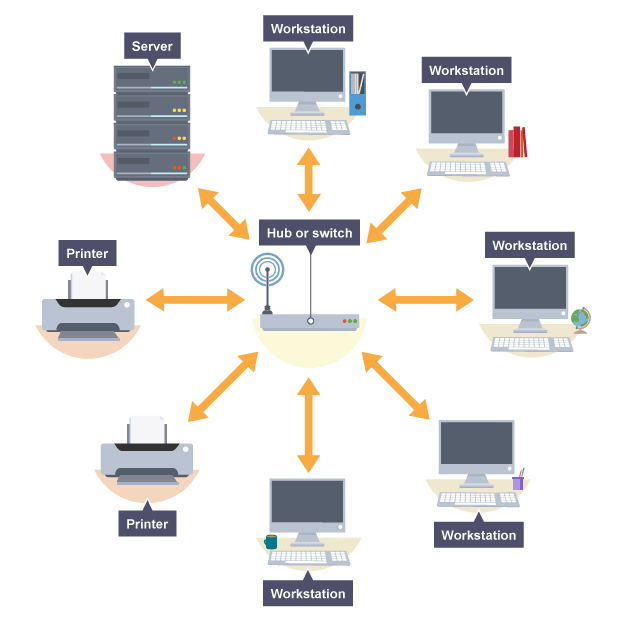
\includegraphics[width=10cm]{./hbs.PNG}
%\vspace{-10pt}
\caption{devices connected together}\label{wrap-fig:5}
\end{wrapfigure}

\subsubsection{Hubs}
A hub broadcasts data to all devices on a network. This can use a lot of \textbf{bandwidth} as it results in unnecessary data being sent - not all computers might need to receive the data. A hub would be useful to link up a few games consoles for a local multiplayer game using a wired LAN.

\wrapfill


\begin{wrapfigure}{L}{8cm}
\centering\newcommand{\wrapfill}{\par\ifnum\value{WF@wrappedlines}>0
  \addtocounter{WF@wrappedlines}{-1}%
  \null\vspace{\arabic{WF@wrappedlines}\baselineskip}%
  \WFclear
\fi}
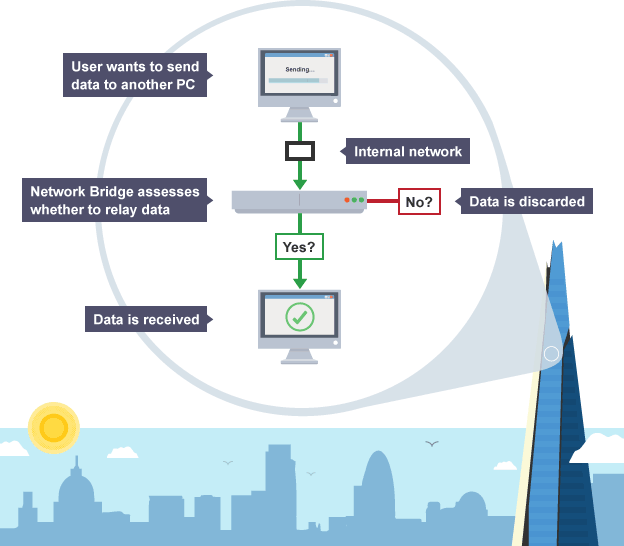
\includegraphics[width=8cm]{./performance.PNG}
\vspace{-10pt}
\caption{Bridge saving unnecessary data transfer}\label{wrap-fig:6}
\end{wrapfigure}


\subsubsection{Bridges}
A \textbf{bridge} is used to connect two separate LAN networks. A computer can act as a bridge through the \textbf{operating system}. A bridge looks for the receiving device before it sends the message. This means that it will not send a message if the receiving computer is not there. It will check to see if the receiver has already had the message. This can help save unnecessary data transfers, which improves the performance of a network.(see Figure 6)

\wrapfill
\clearpage

\subsubsection{Switches}
A \textbf{switch} performs a similar role to a hub and a bridge but is more powerful. It stores the \textbf{MAC addresses} of devices on a network and filters \textbf{data packets} to see which devices have asked for them. This makes a switch more efficient when demand is high. If, for example, a game involved lots of data being passed between machines, then a switch could reduce the amount of \textbf{latency}

\section{Cisco Packet Tracer}

Packet Tracer is a cross-platform visual simulation tool designed by Cisco Systems that allows users to create network topologies and imitate modern computer networks. The software allows users to simulate the configuration of Cisco routers and switches using a simulated command line interface. Packet Tracer makes use of a drag and drop user interface, allowing users to add and remove simulated network devices as they see fit. The software is mainly focused towards Cisco Networking Academy students as an educational tool for helping them learn fundamental CCNA concepts. Previously students enrolled in a CCNA Academy program could freely download and use the tool free of charge for educational use.\footnotemark{} \newline

In this experiment we try to ping devices being set with 0 in the IP fields. Then we're gonna expand the network with more devices

\footnotetext{Bakni, Michel; Cardinale, Yudith; Moreno, Luis Manuel (June 2018). \textbf{An Approach to Evaluate Network Simulators: An Experience with Packet Tracer}.Revista Venezolana de Computación. 5: 29–36. ISSN 2244-7040. \newline Javid,Sheikh Raashid (May 2014). \textbf{Role of Packet Tracer in learning Computer Networks} (PDF). International Journal of Advanced Research in Computer and Communication Engineering. 3 (5): 6508–6511.}

\begin{itemize}
\item{First nextwork has a 192.168.1.1 default gateway}
\item{Second network has a 192.168.0.1 default gateway}
\end{itemize}

\clearpage

\subsection{The step-by-step guide}

\href{https://monsterhunter.fandom.com/wiki/Seregios}{Seregios}\footnote{\label{seregios}Seregios is a Flying Wyvern introduced in \href{https://monsterhunter.fandom.com/wiki/Monster_Hunter_4_Ultimate}{Monster Hunter 4 Ultimate}.} wants to create a network on Cisco Packet Tracer. The task is quite easy but he's got quite a few tasks to accomplish

\begin{wrapfigure}{3cm}
\centering
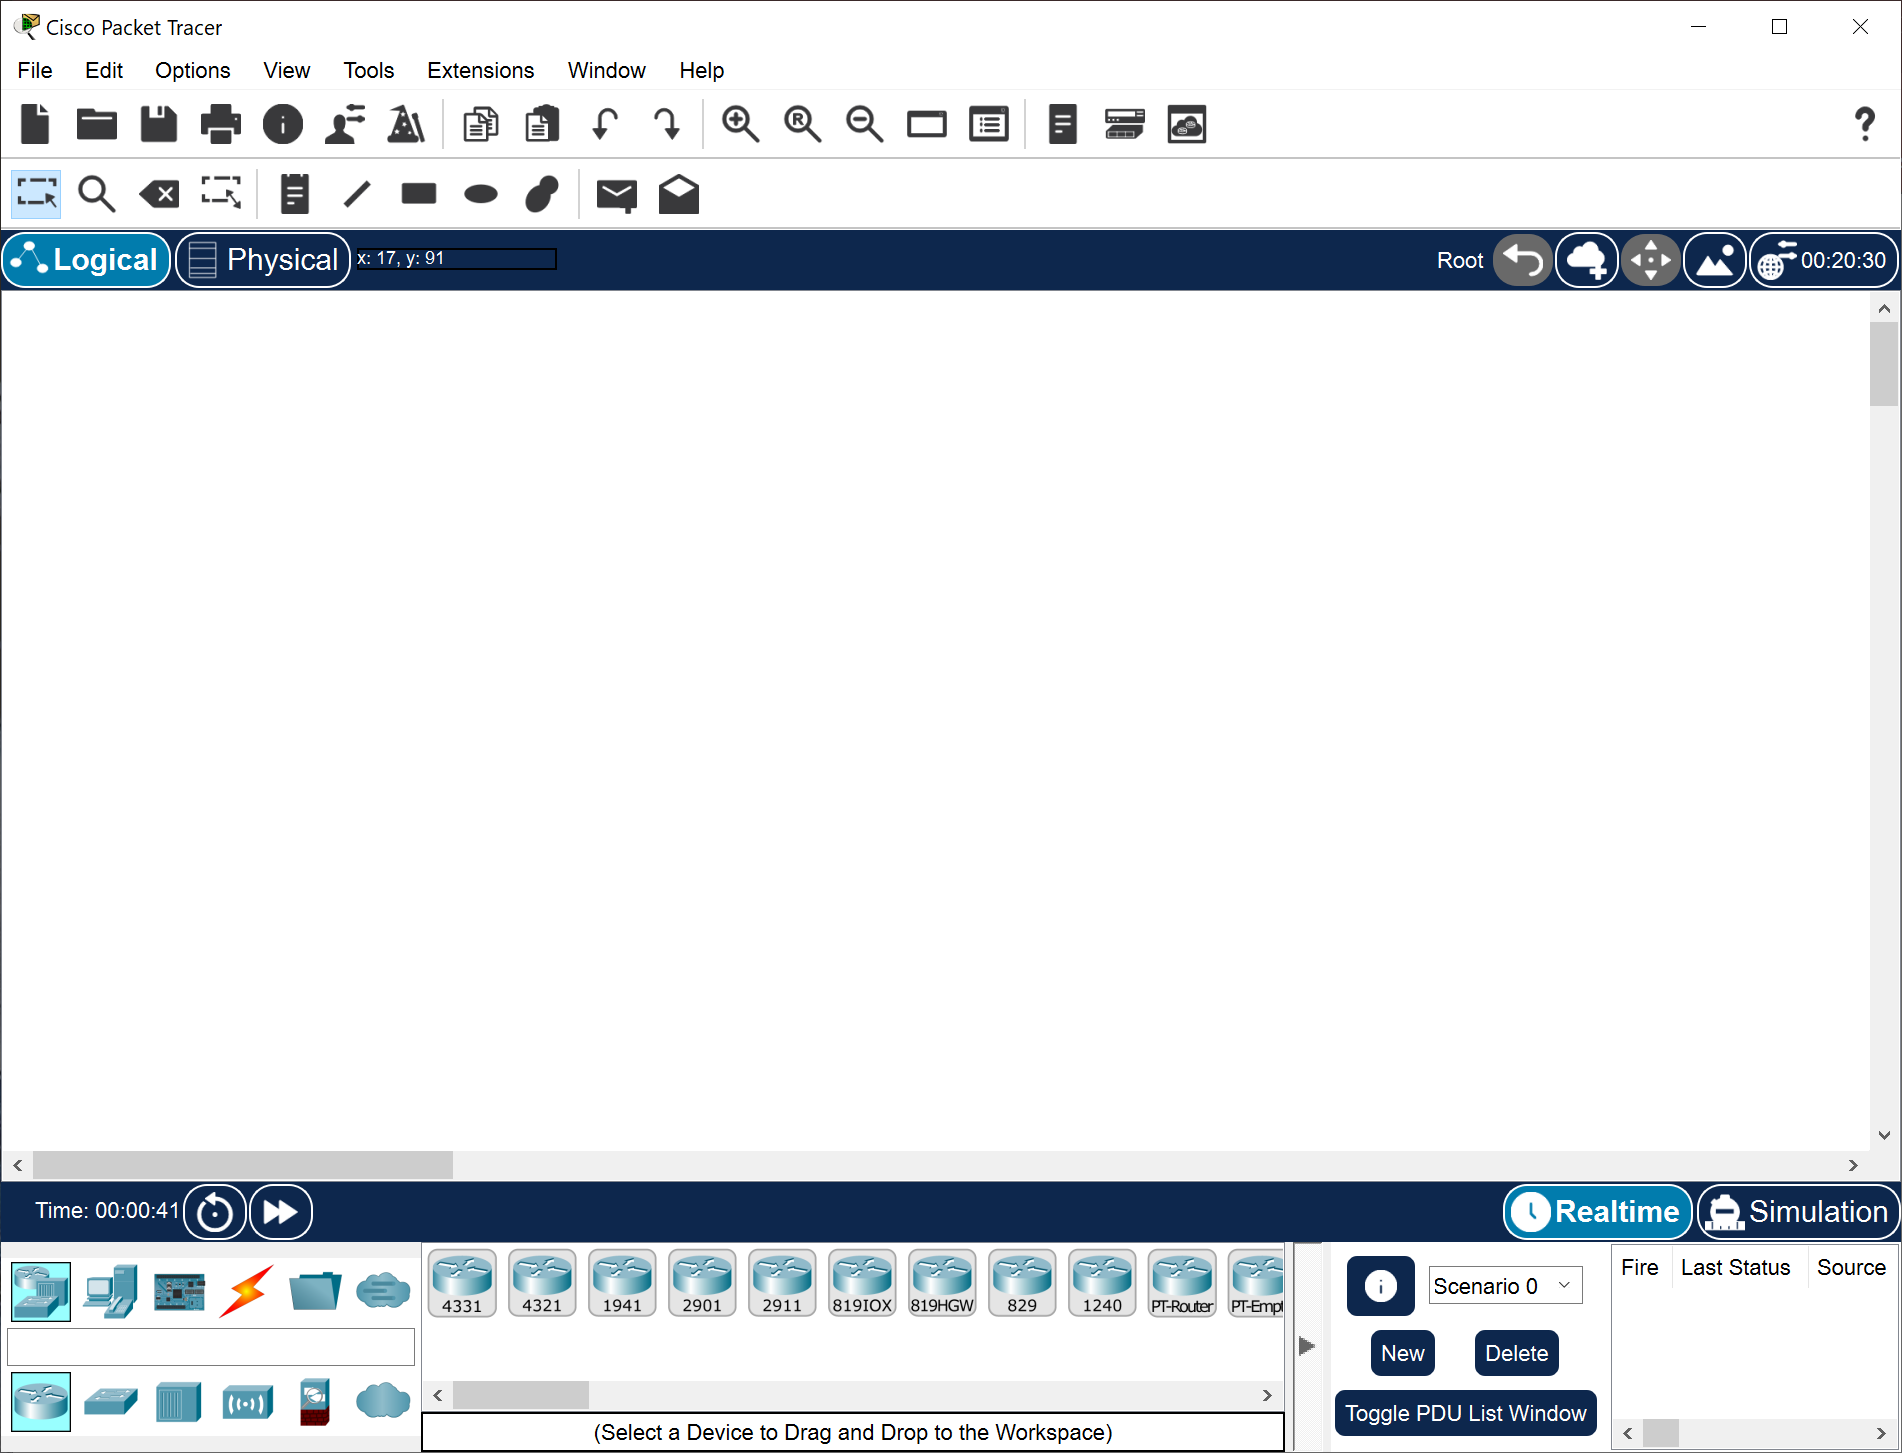
\includegraphics[width=13cm]{./step-by-step/0.PNG}
%\vspace{-10pt}
\caption{first screen he gets when he opens Cisco Packet Tracer}\label{wrap-fig:100}
\end{wrapfigure}

The first he needs to do is opening Cisco Packet Tracer. The screen will be completely empty with no devices selected. On the right hand side of the bottom panel \textbf{Realtime} is being selected instead of \textbf{Simulation} \newline

\clearpage

\noindent Now what he needs to do is to add a switch : \newline

\noindent 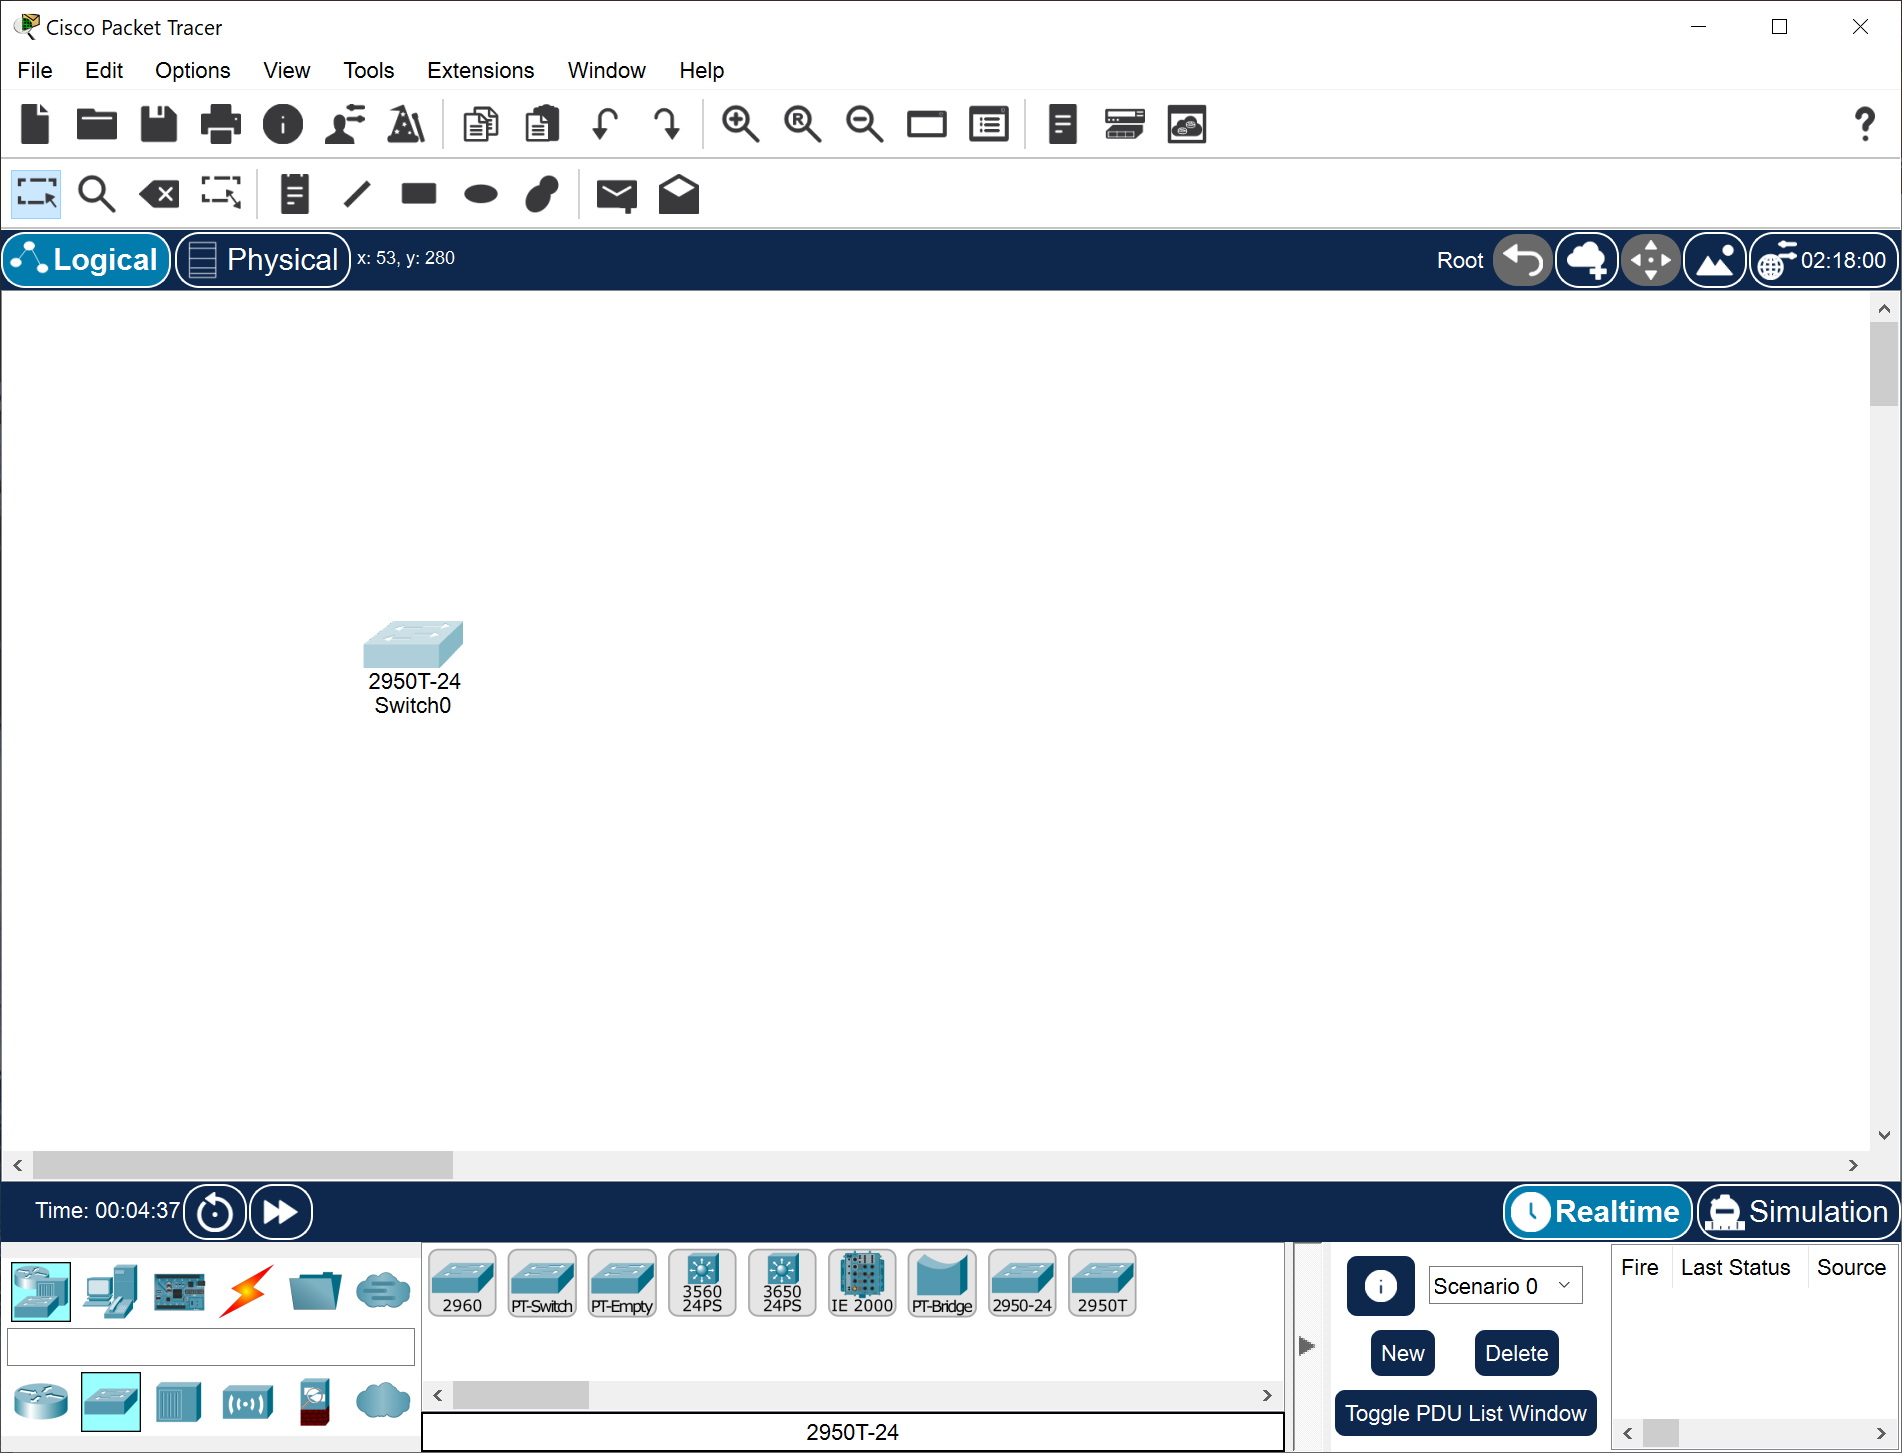
\includegraphics[width=13cm]{./step-by-step/1.PNG}
\clearpage

\noindent And then we add a computer : \newline

\noindent 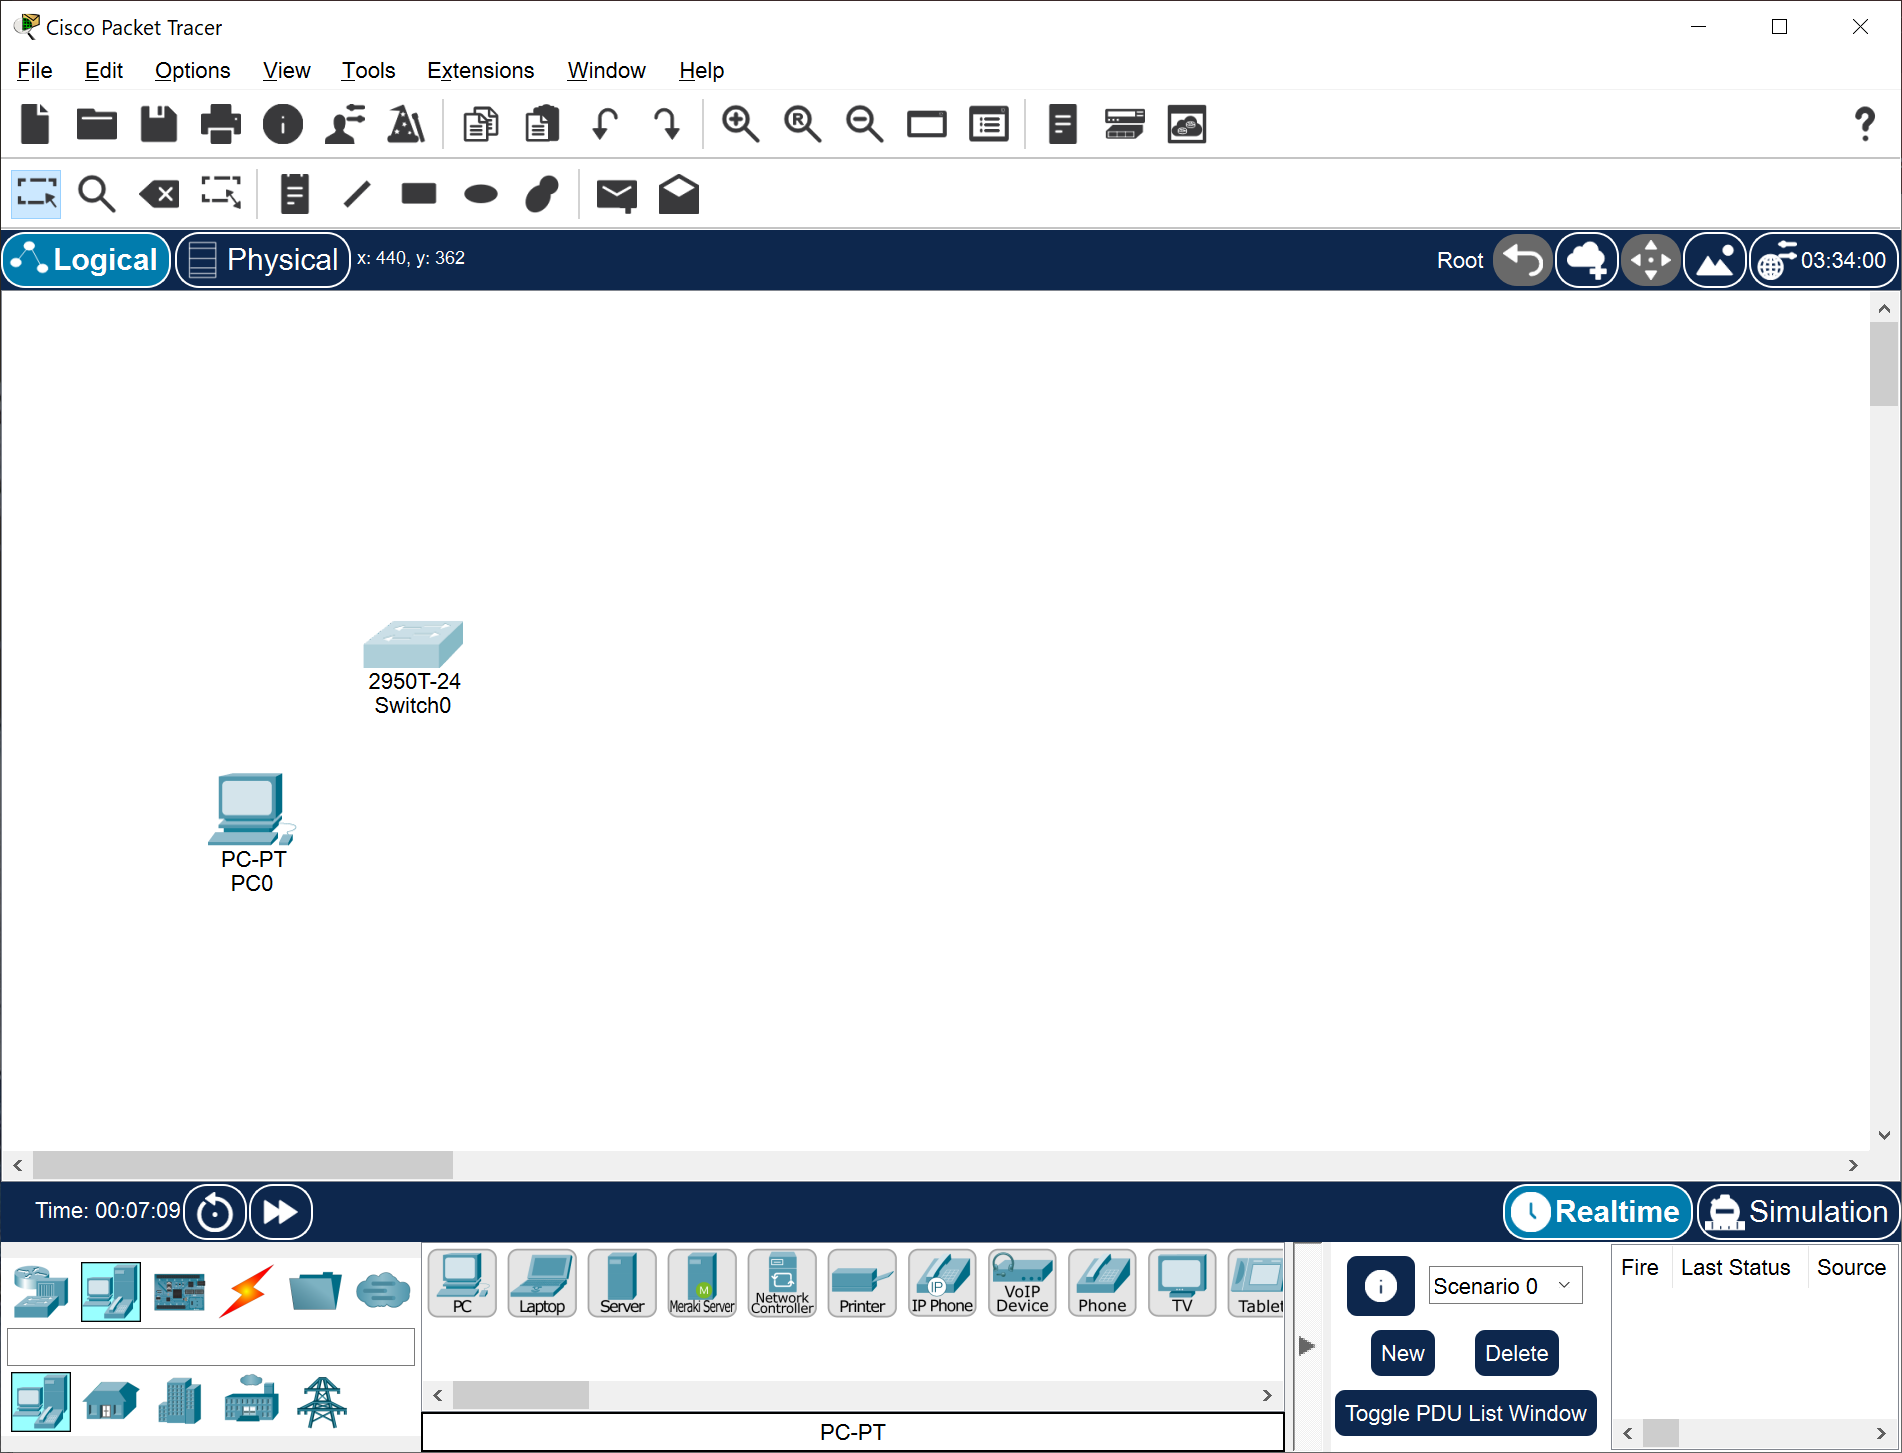
\includegraphics[width=13cm]{./step-by-step/2.PNG}
\clearpage

\noindent Now we click on the computer \newline

\noindent 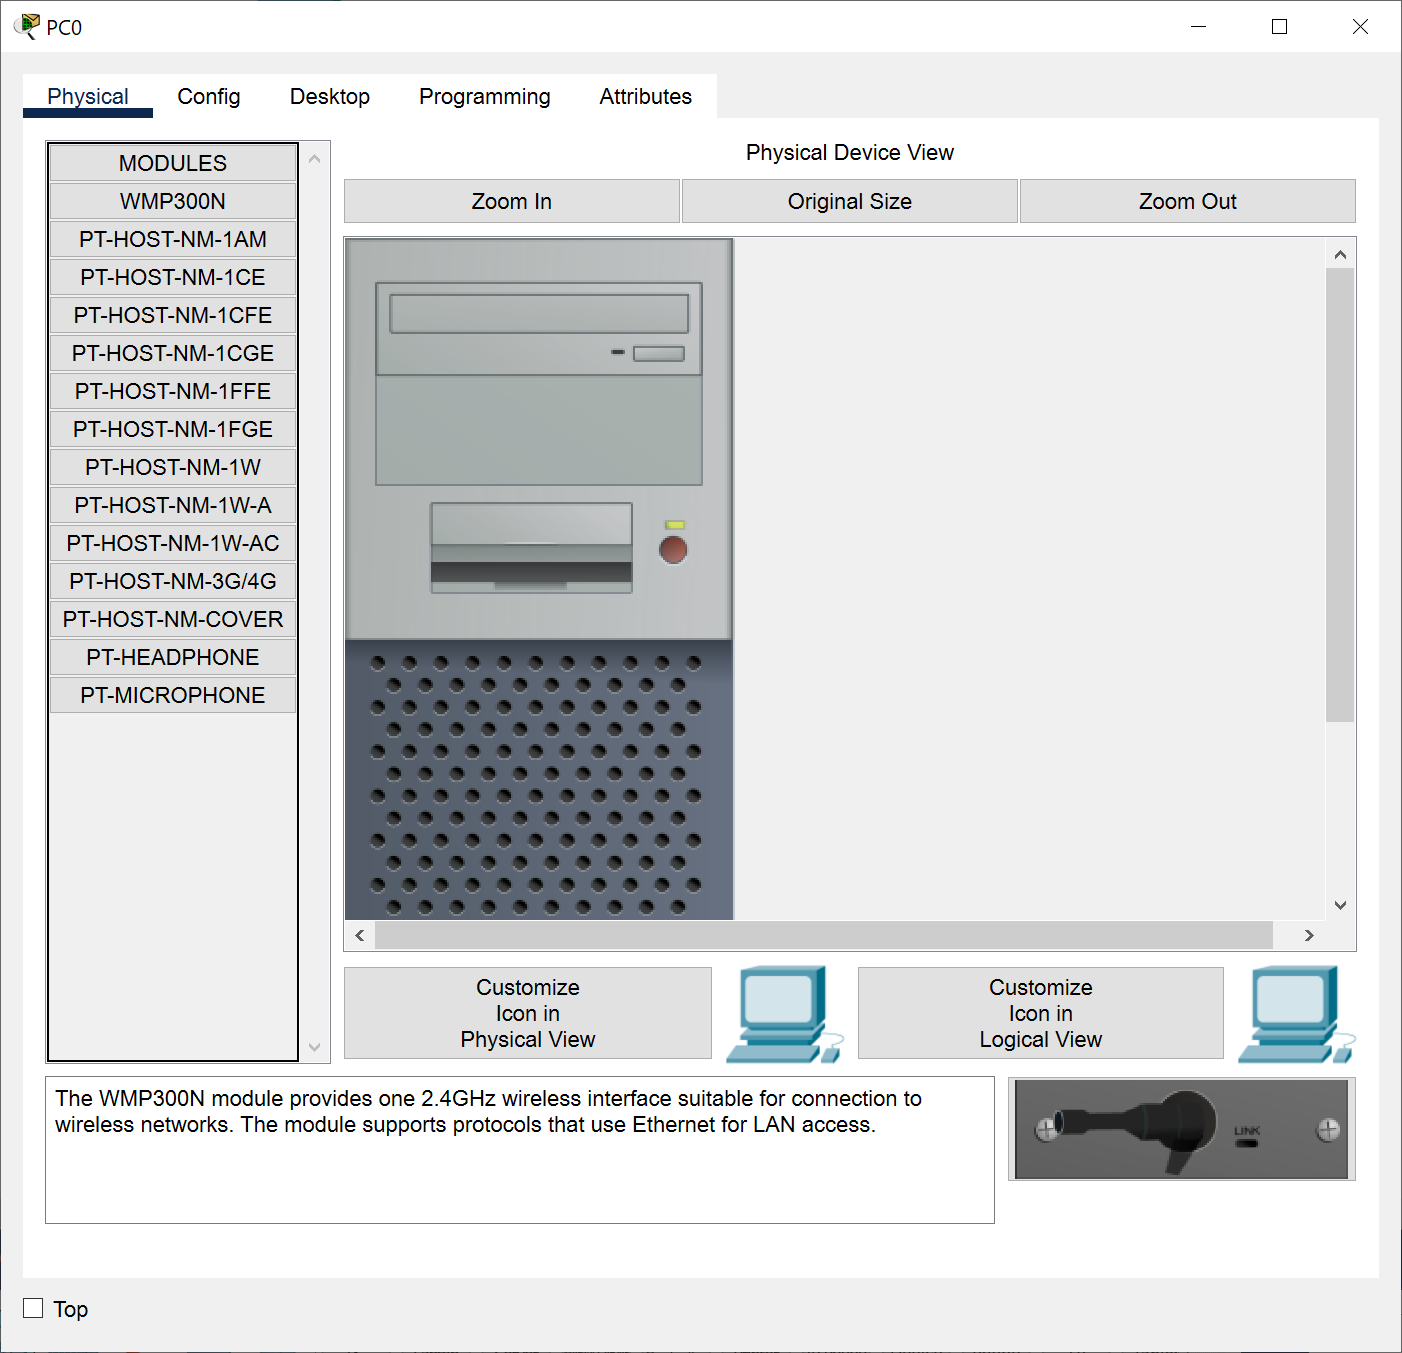
\includegraphics[width=13cm]{./step-by-step/3.PNG}
\clearpage

\noindent And we move ourselves in the \textvg{Config} tab \newline

\noindent 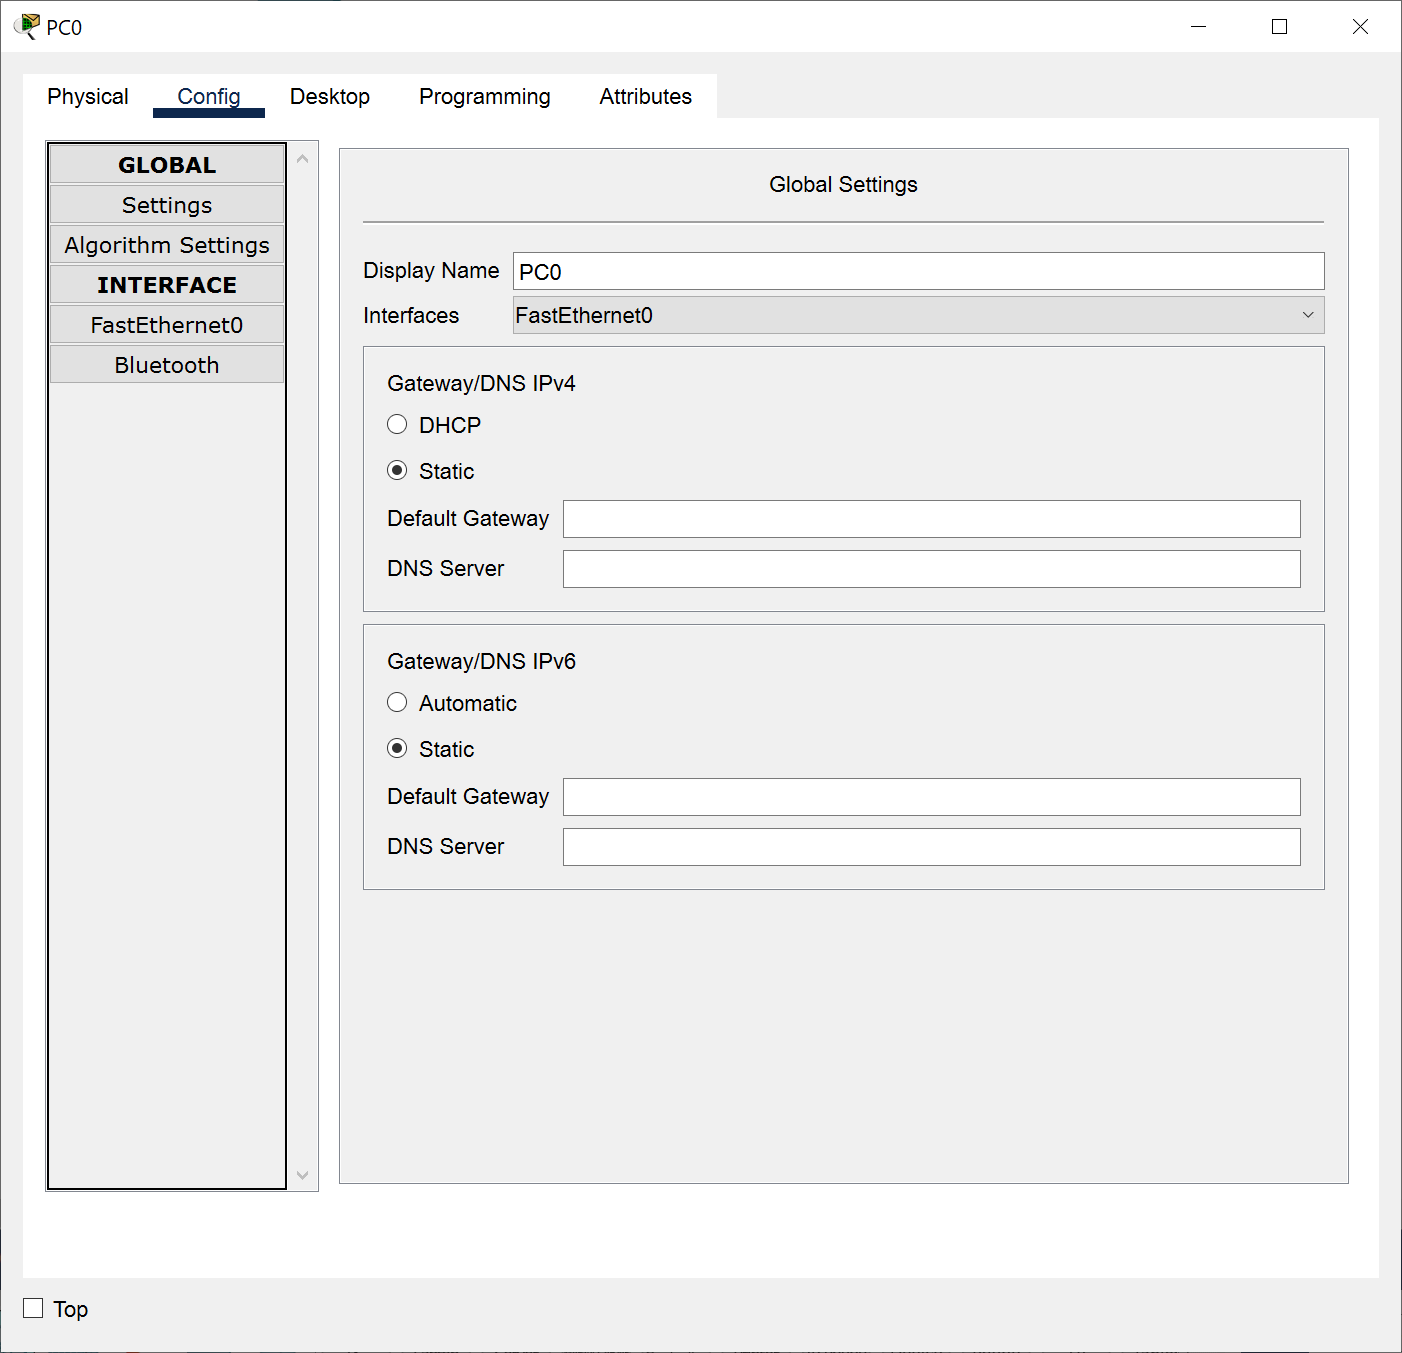
\includegraphics[width=13cm]{./step-by-step/4.PNG}
\clearpage

\noindent what we're gonna be looking later at is the IPV4 address \newline

\noindent 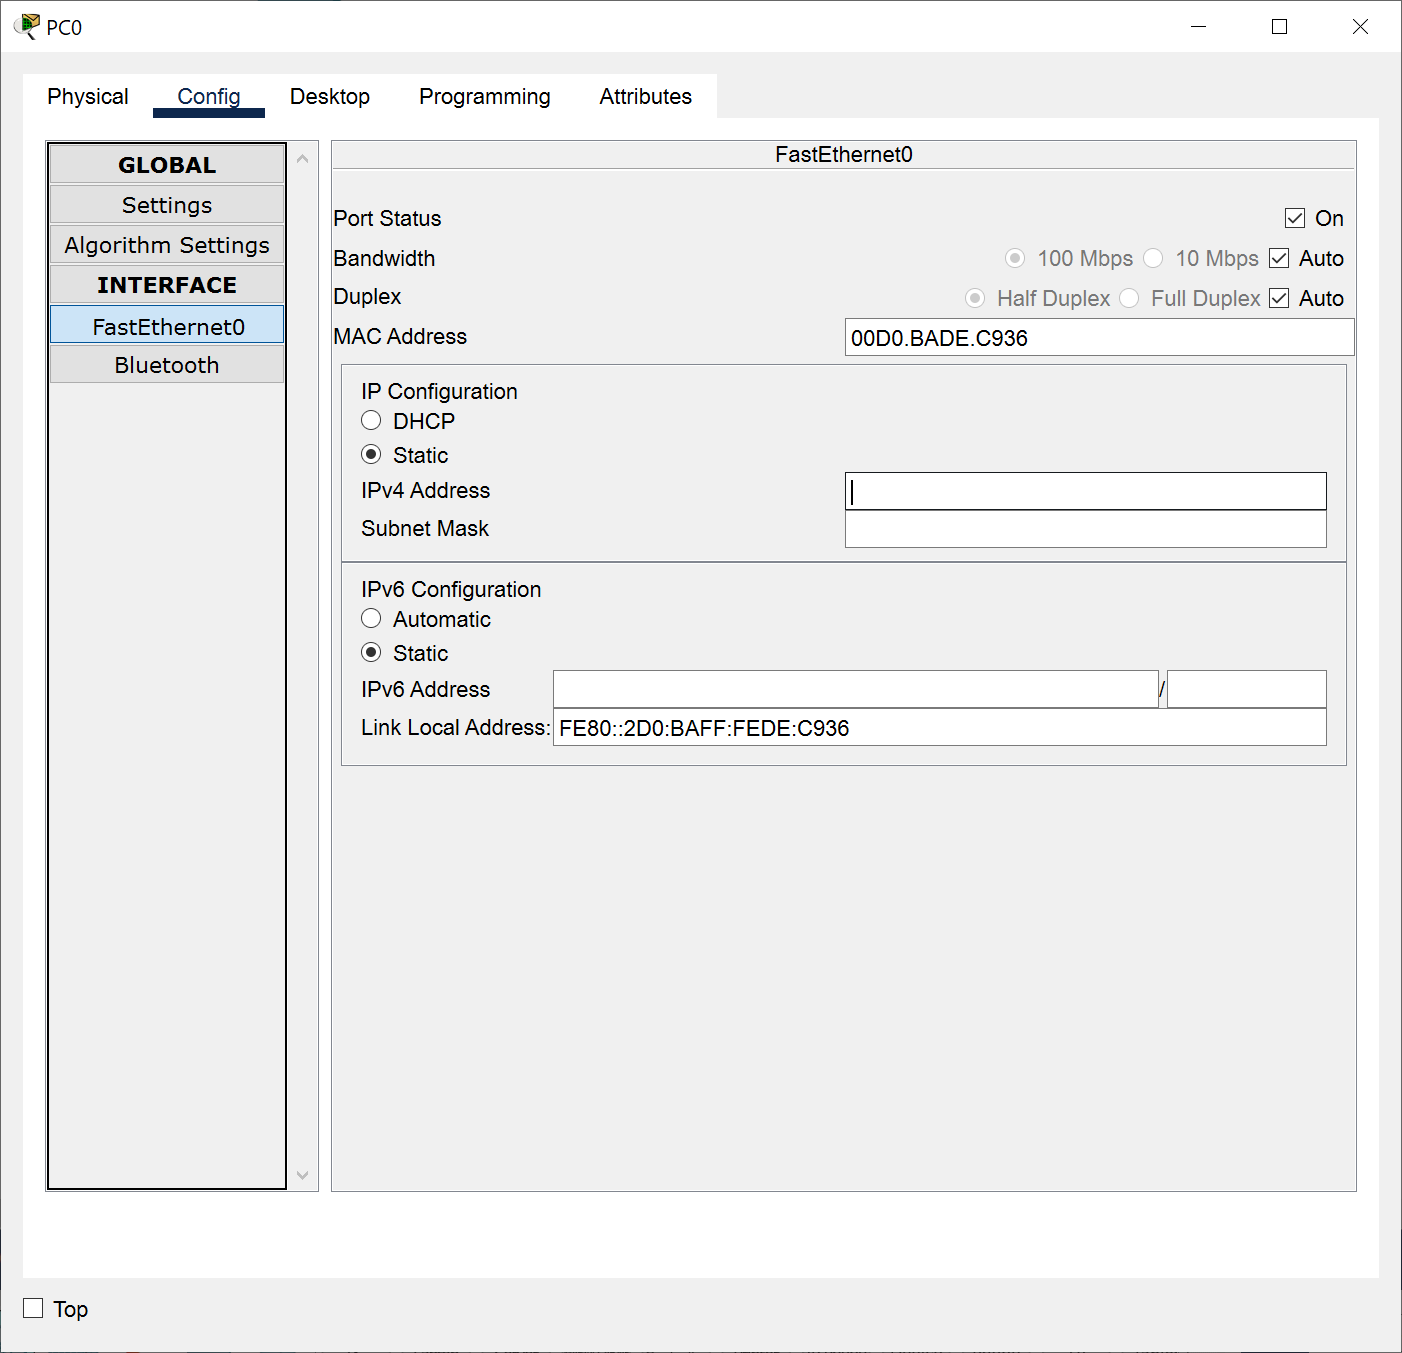
\includegraphics[width=13cm]{./step-by-step/5.PNG}
\clearpage

\noindent in the meantime let's  go in global and set the \textbf{IP Address} equal to this 

\[192.168.0.1\]

\noindent 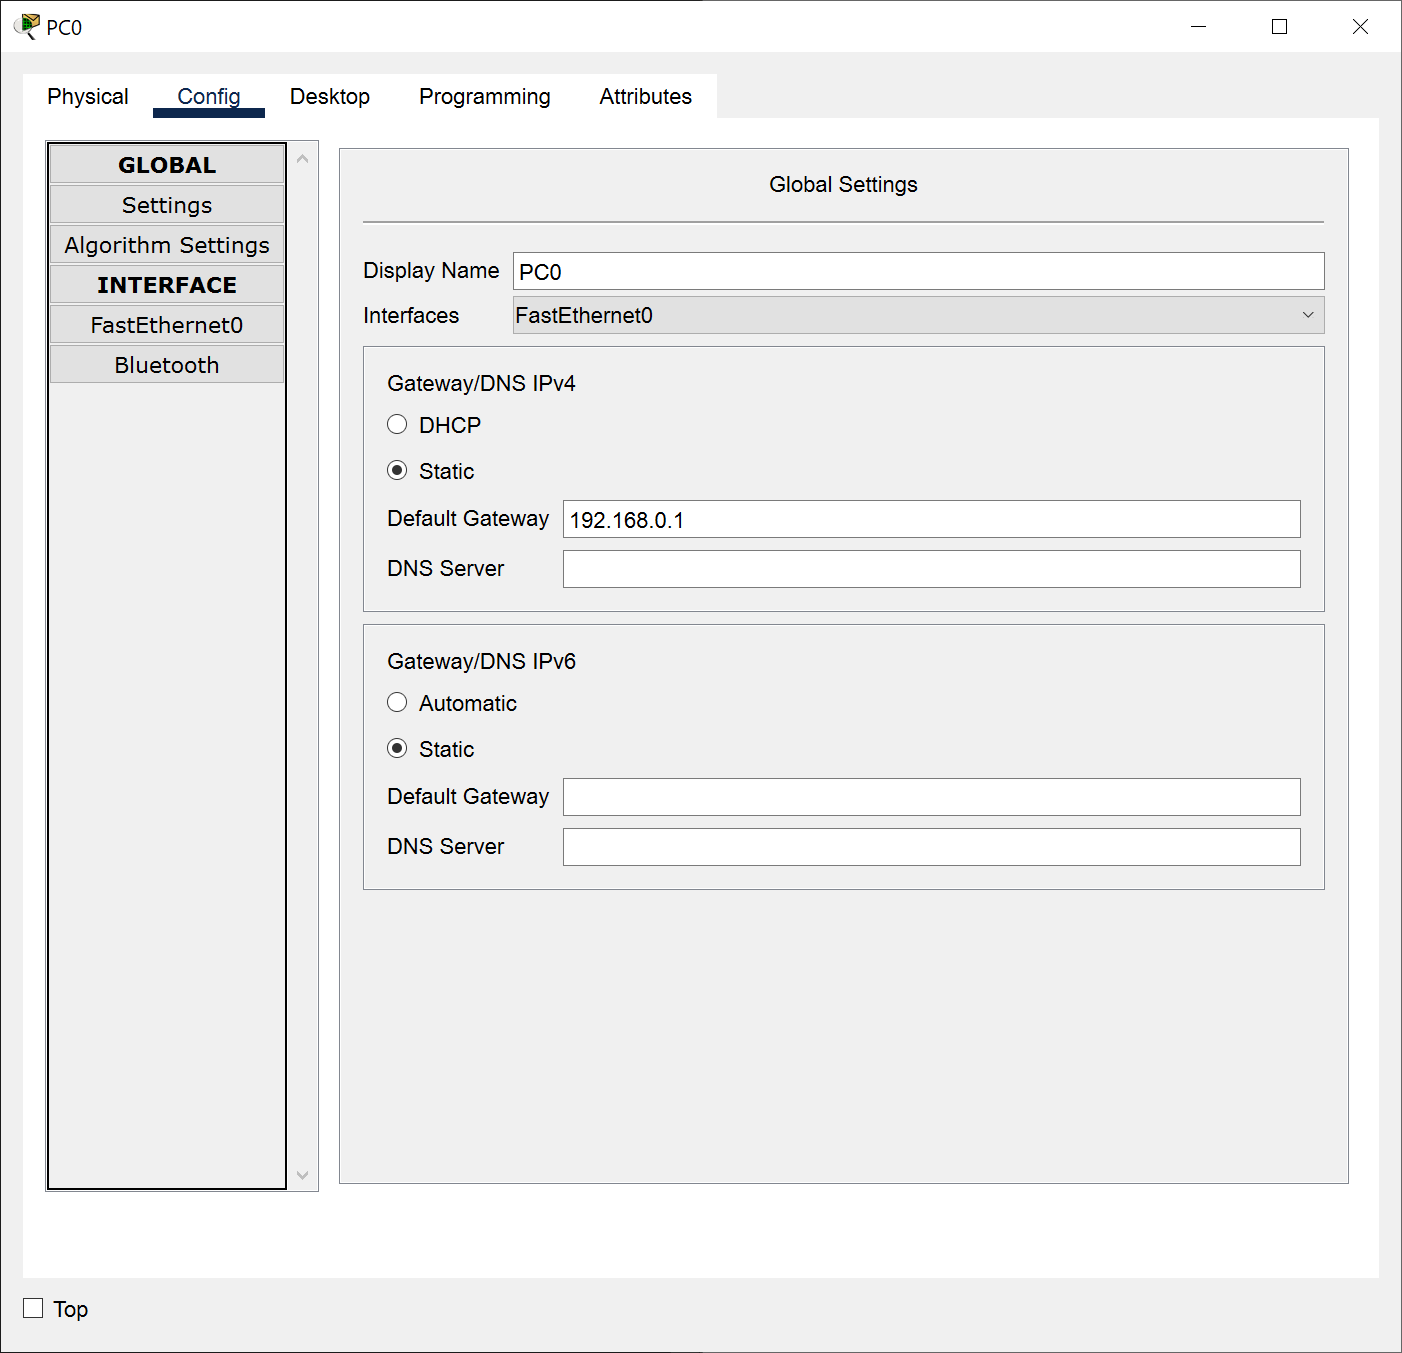
\includegraphics[width=13cm]{./step-by-step/6.PNG}
\clearpage

\noindent Now we add a new computer \newline

\noindent 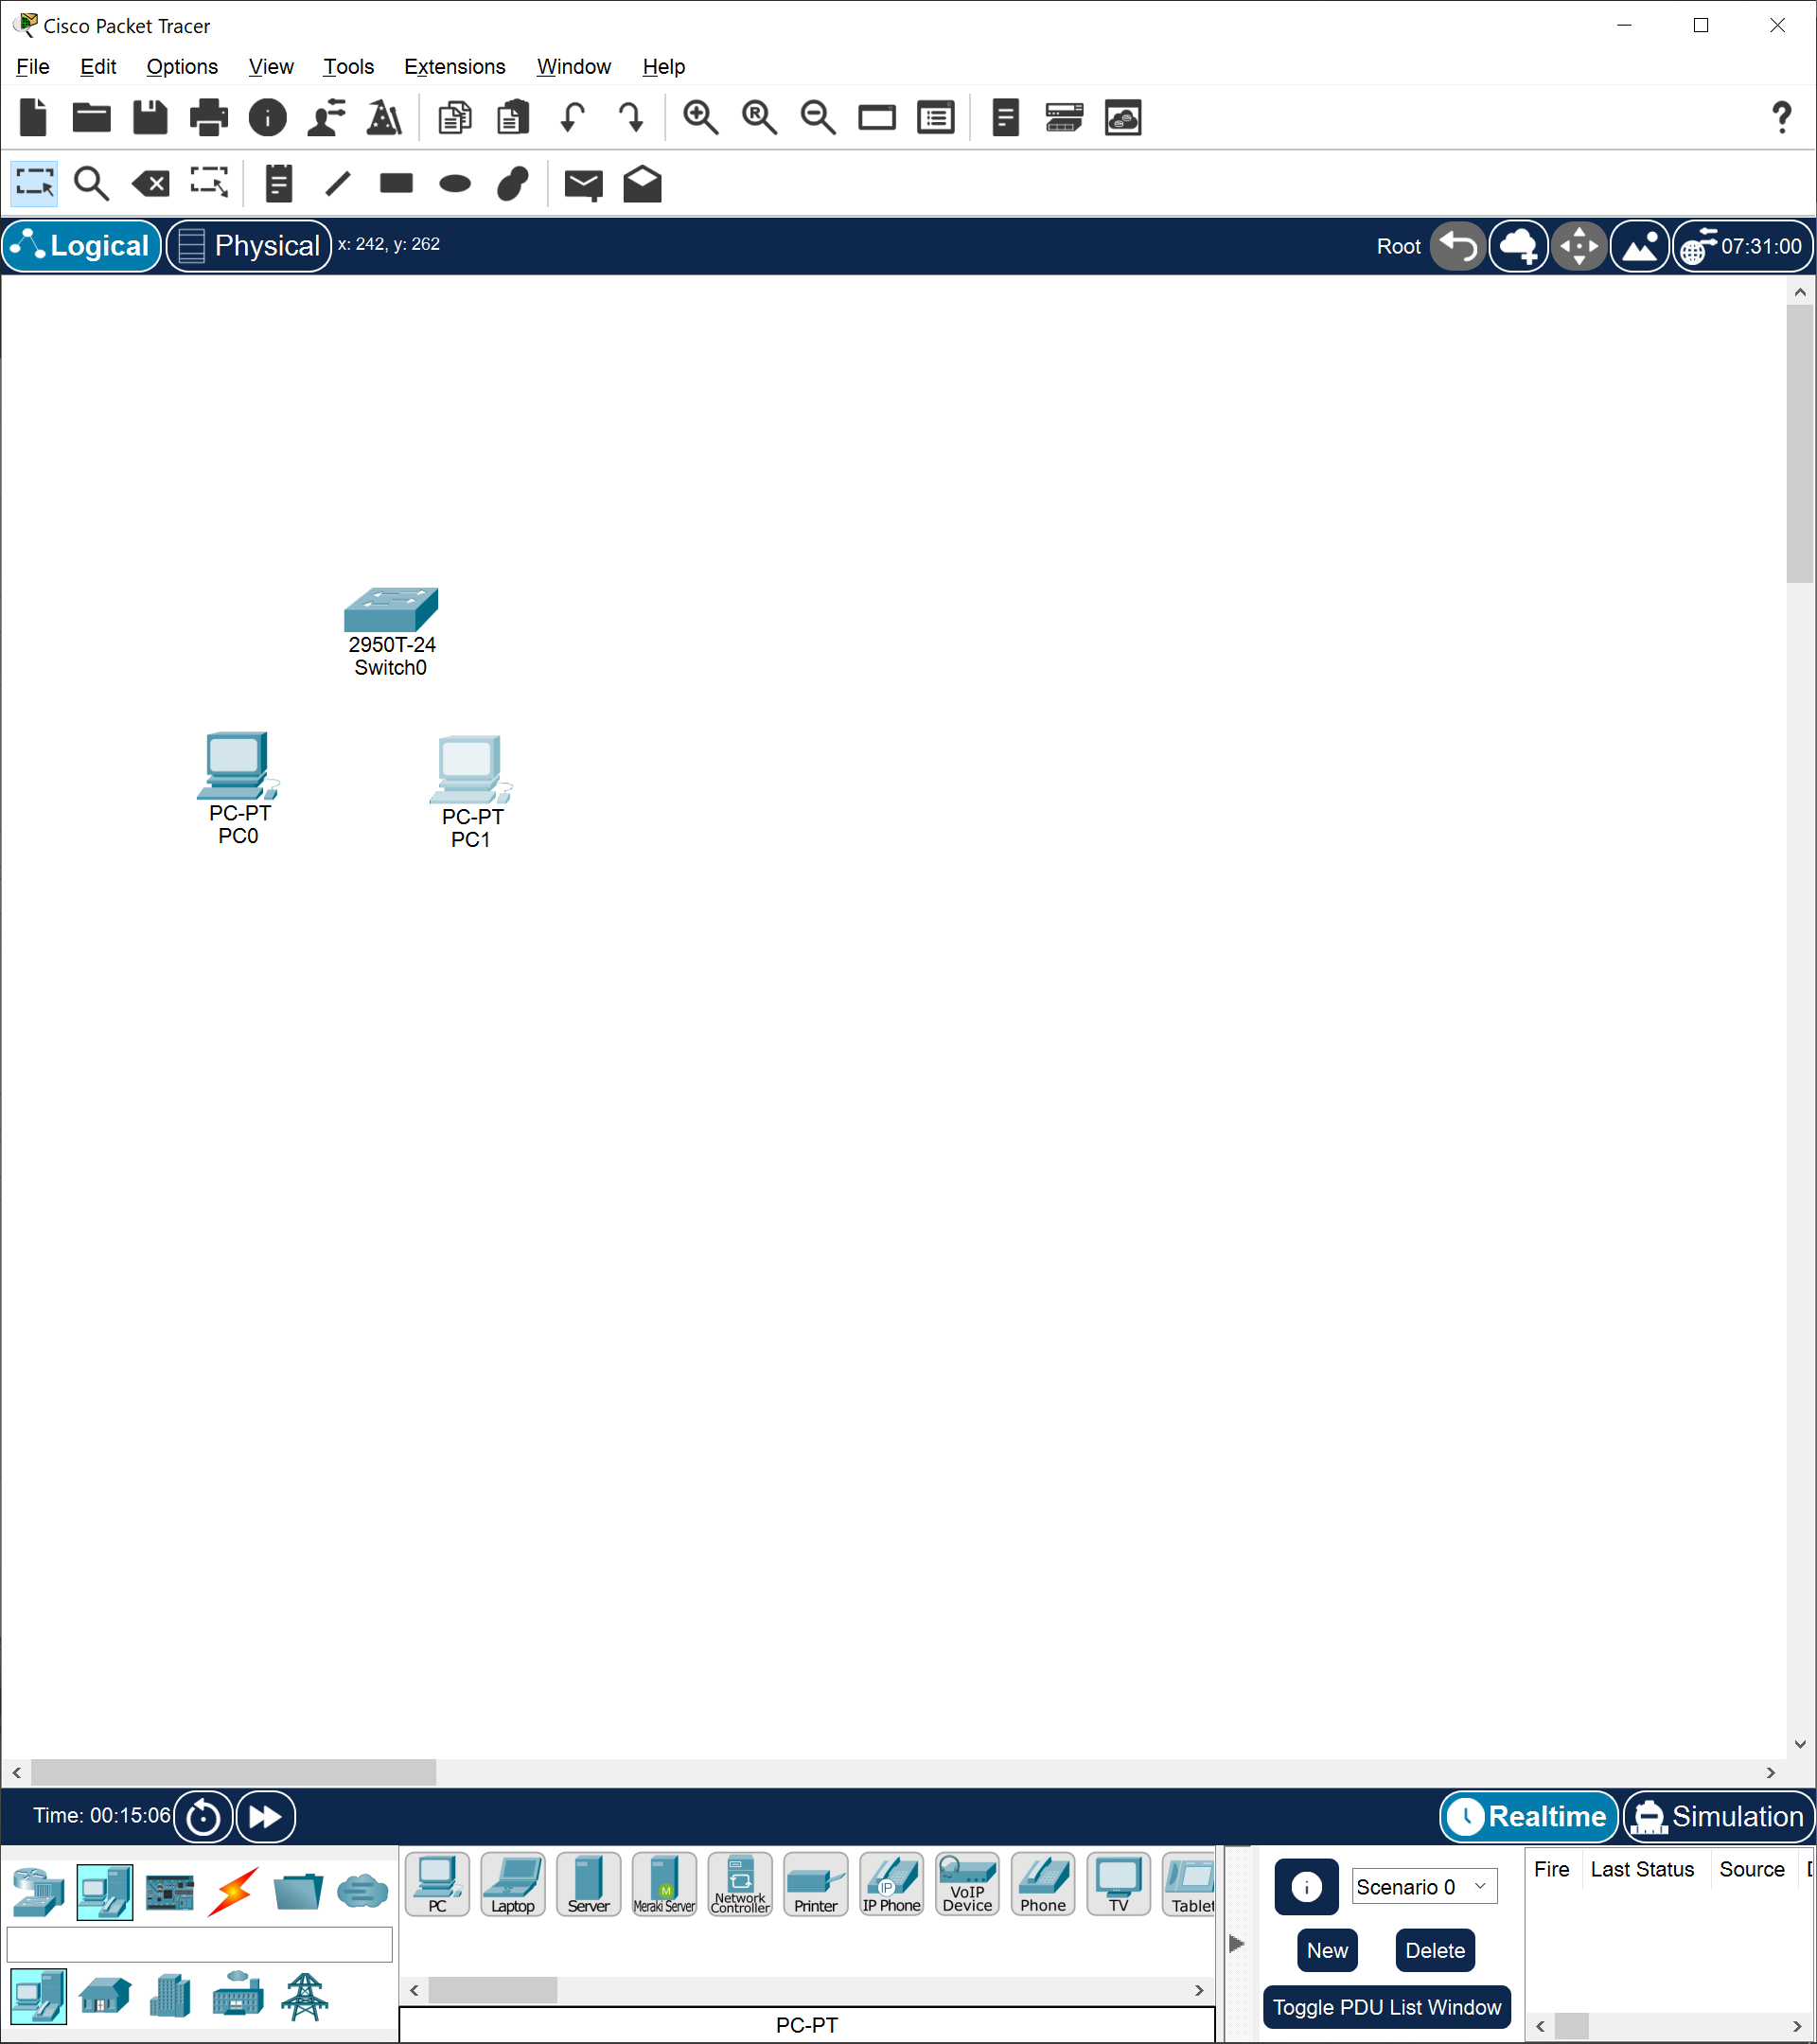
\includegraphics[width=13cm]{./step-by-step/7.PNG}
\clearpage


\noindent We link the switch to the first computer and wait for all lights to go green \newline

\noindent 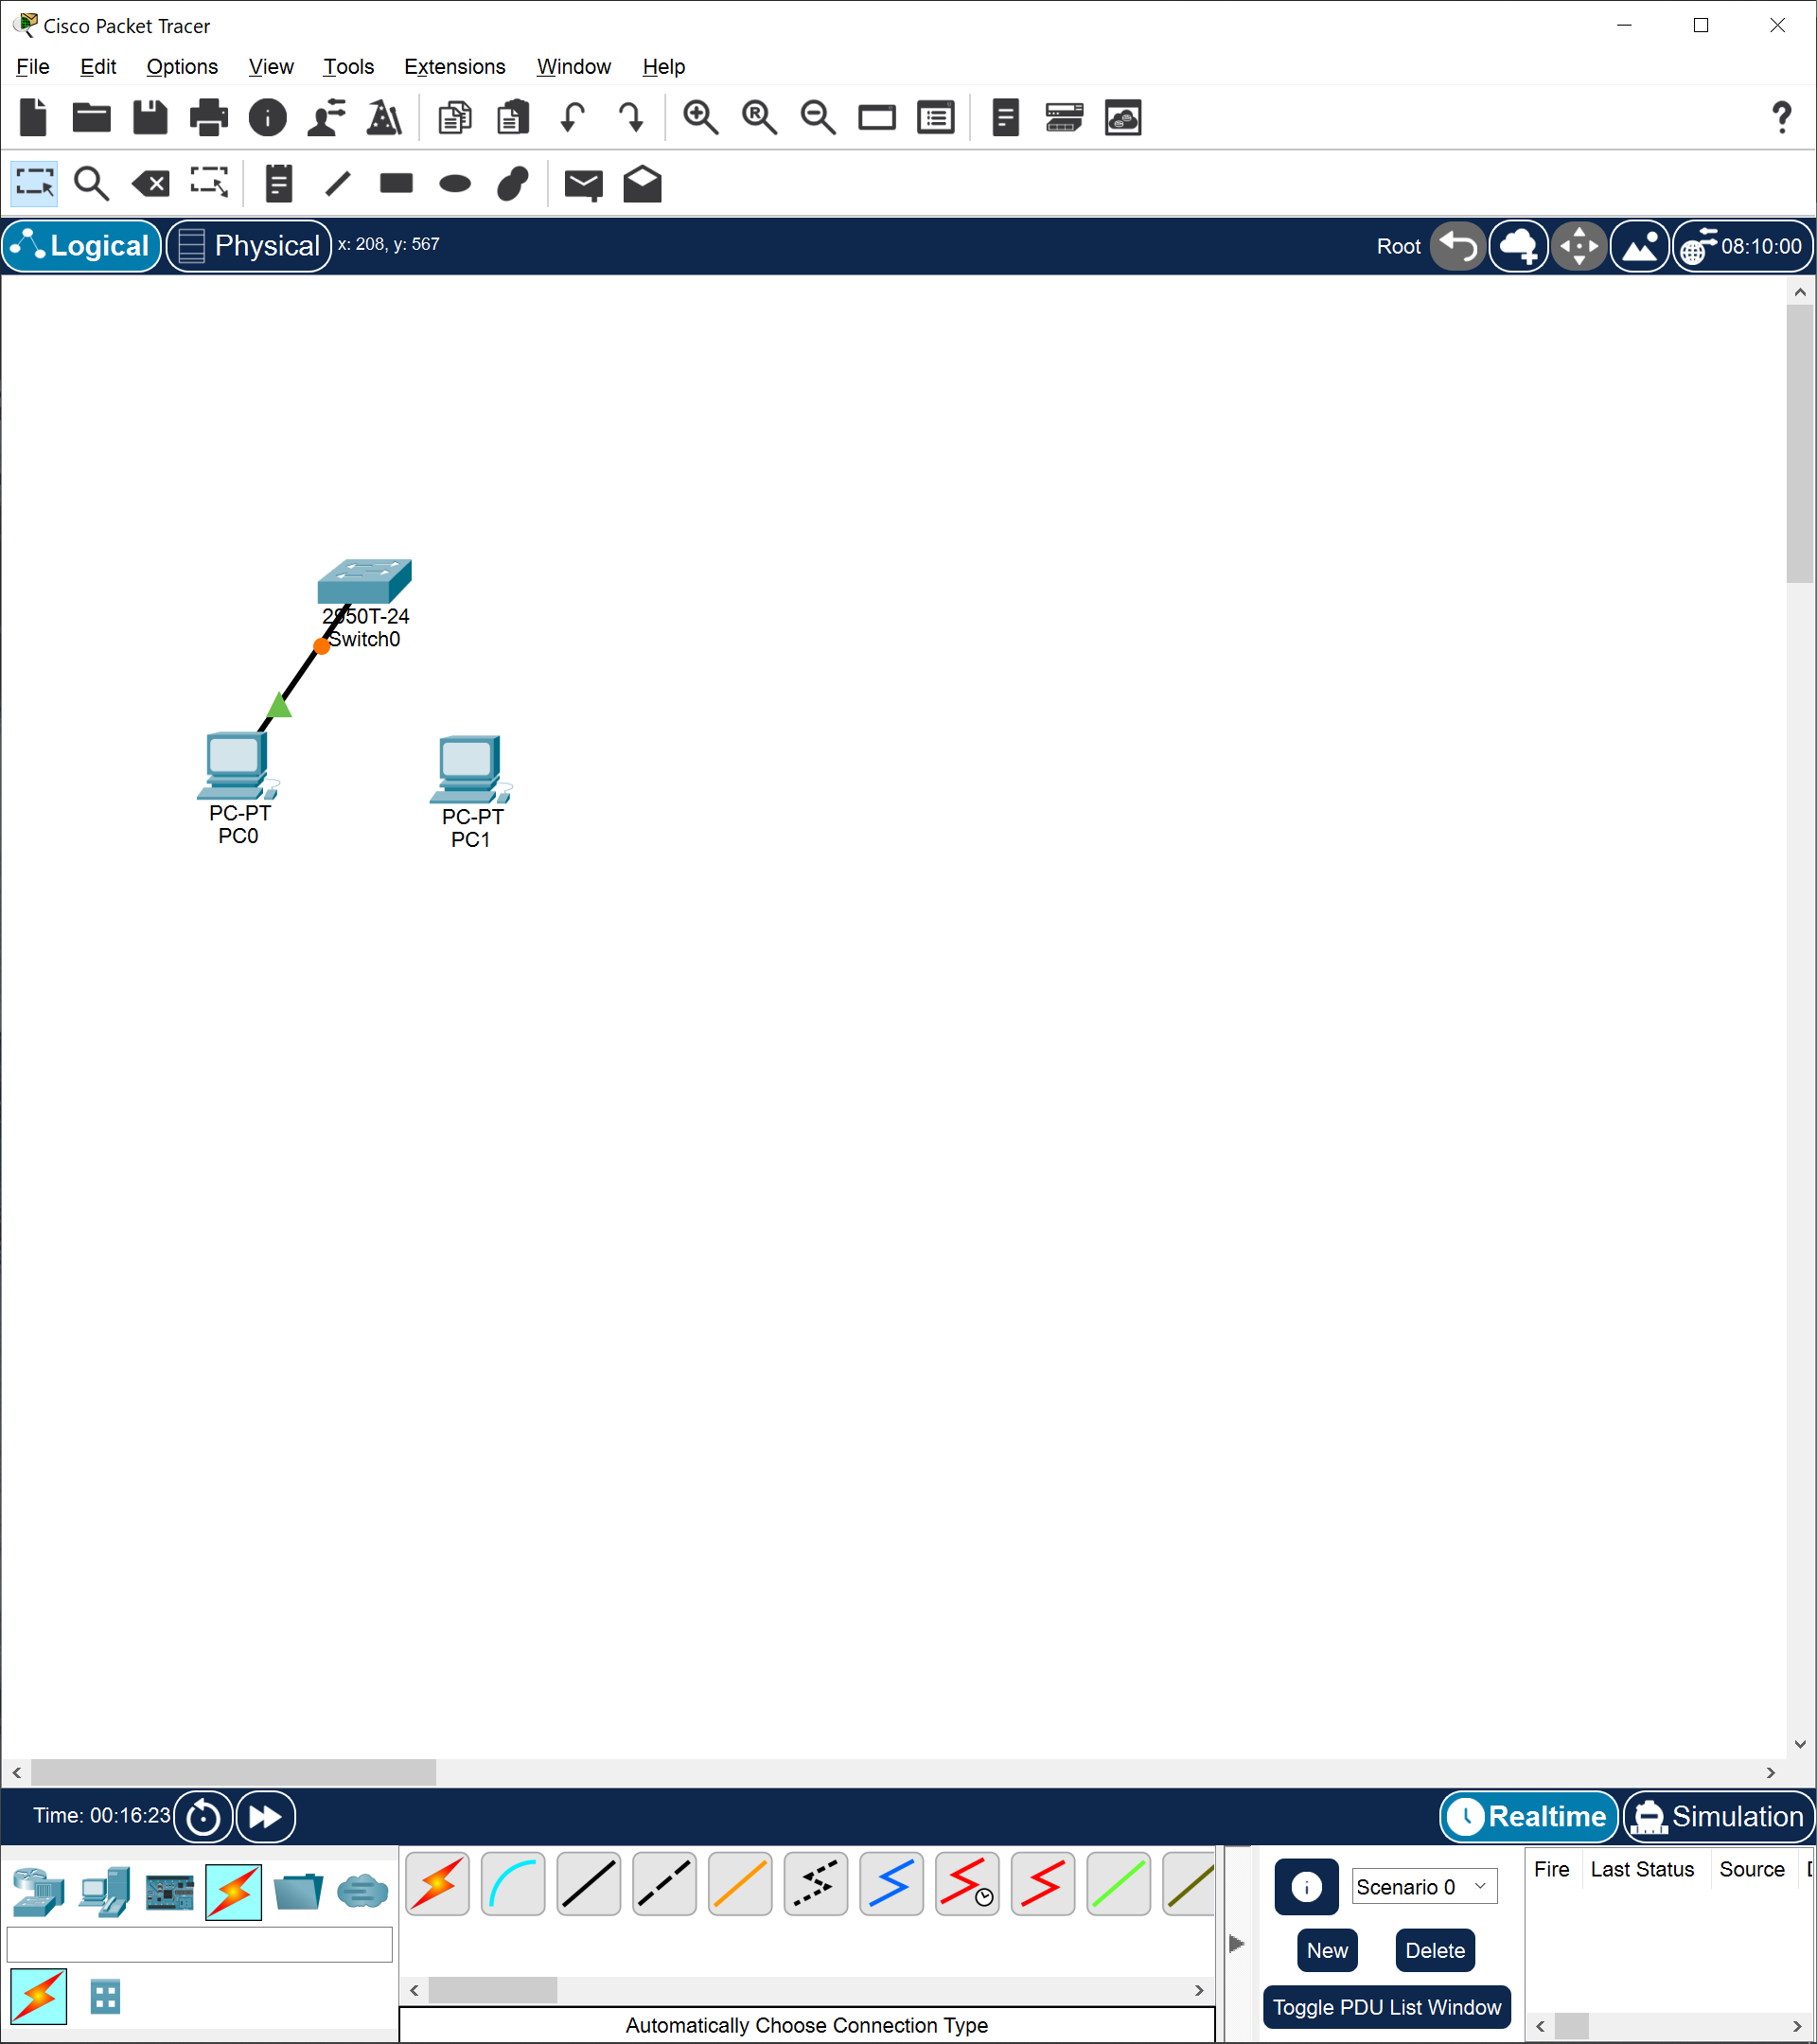
\includegraphics[width=13cm]{./step-by-step/8.PNG}
\clearpage

\noindent Link the switch to the second computer and wait for this link to go all green as well \newline

\noindent 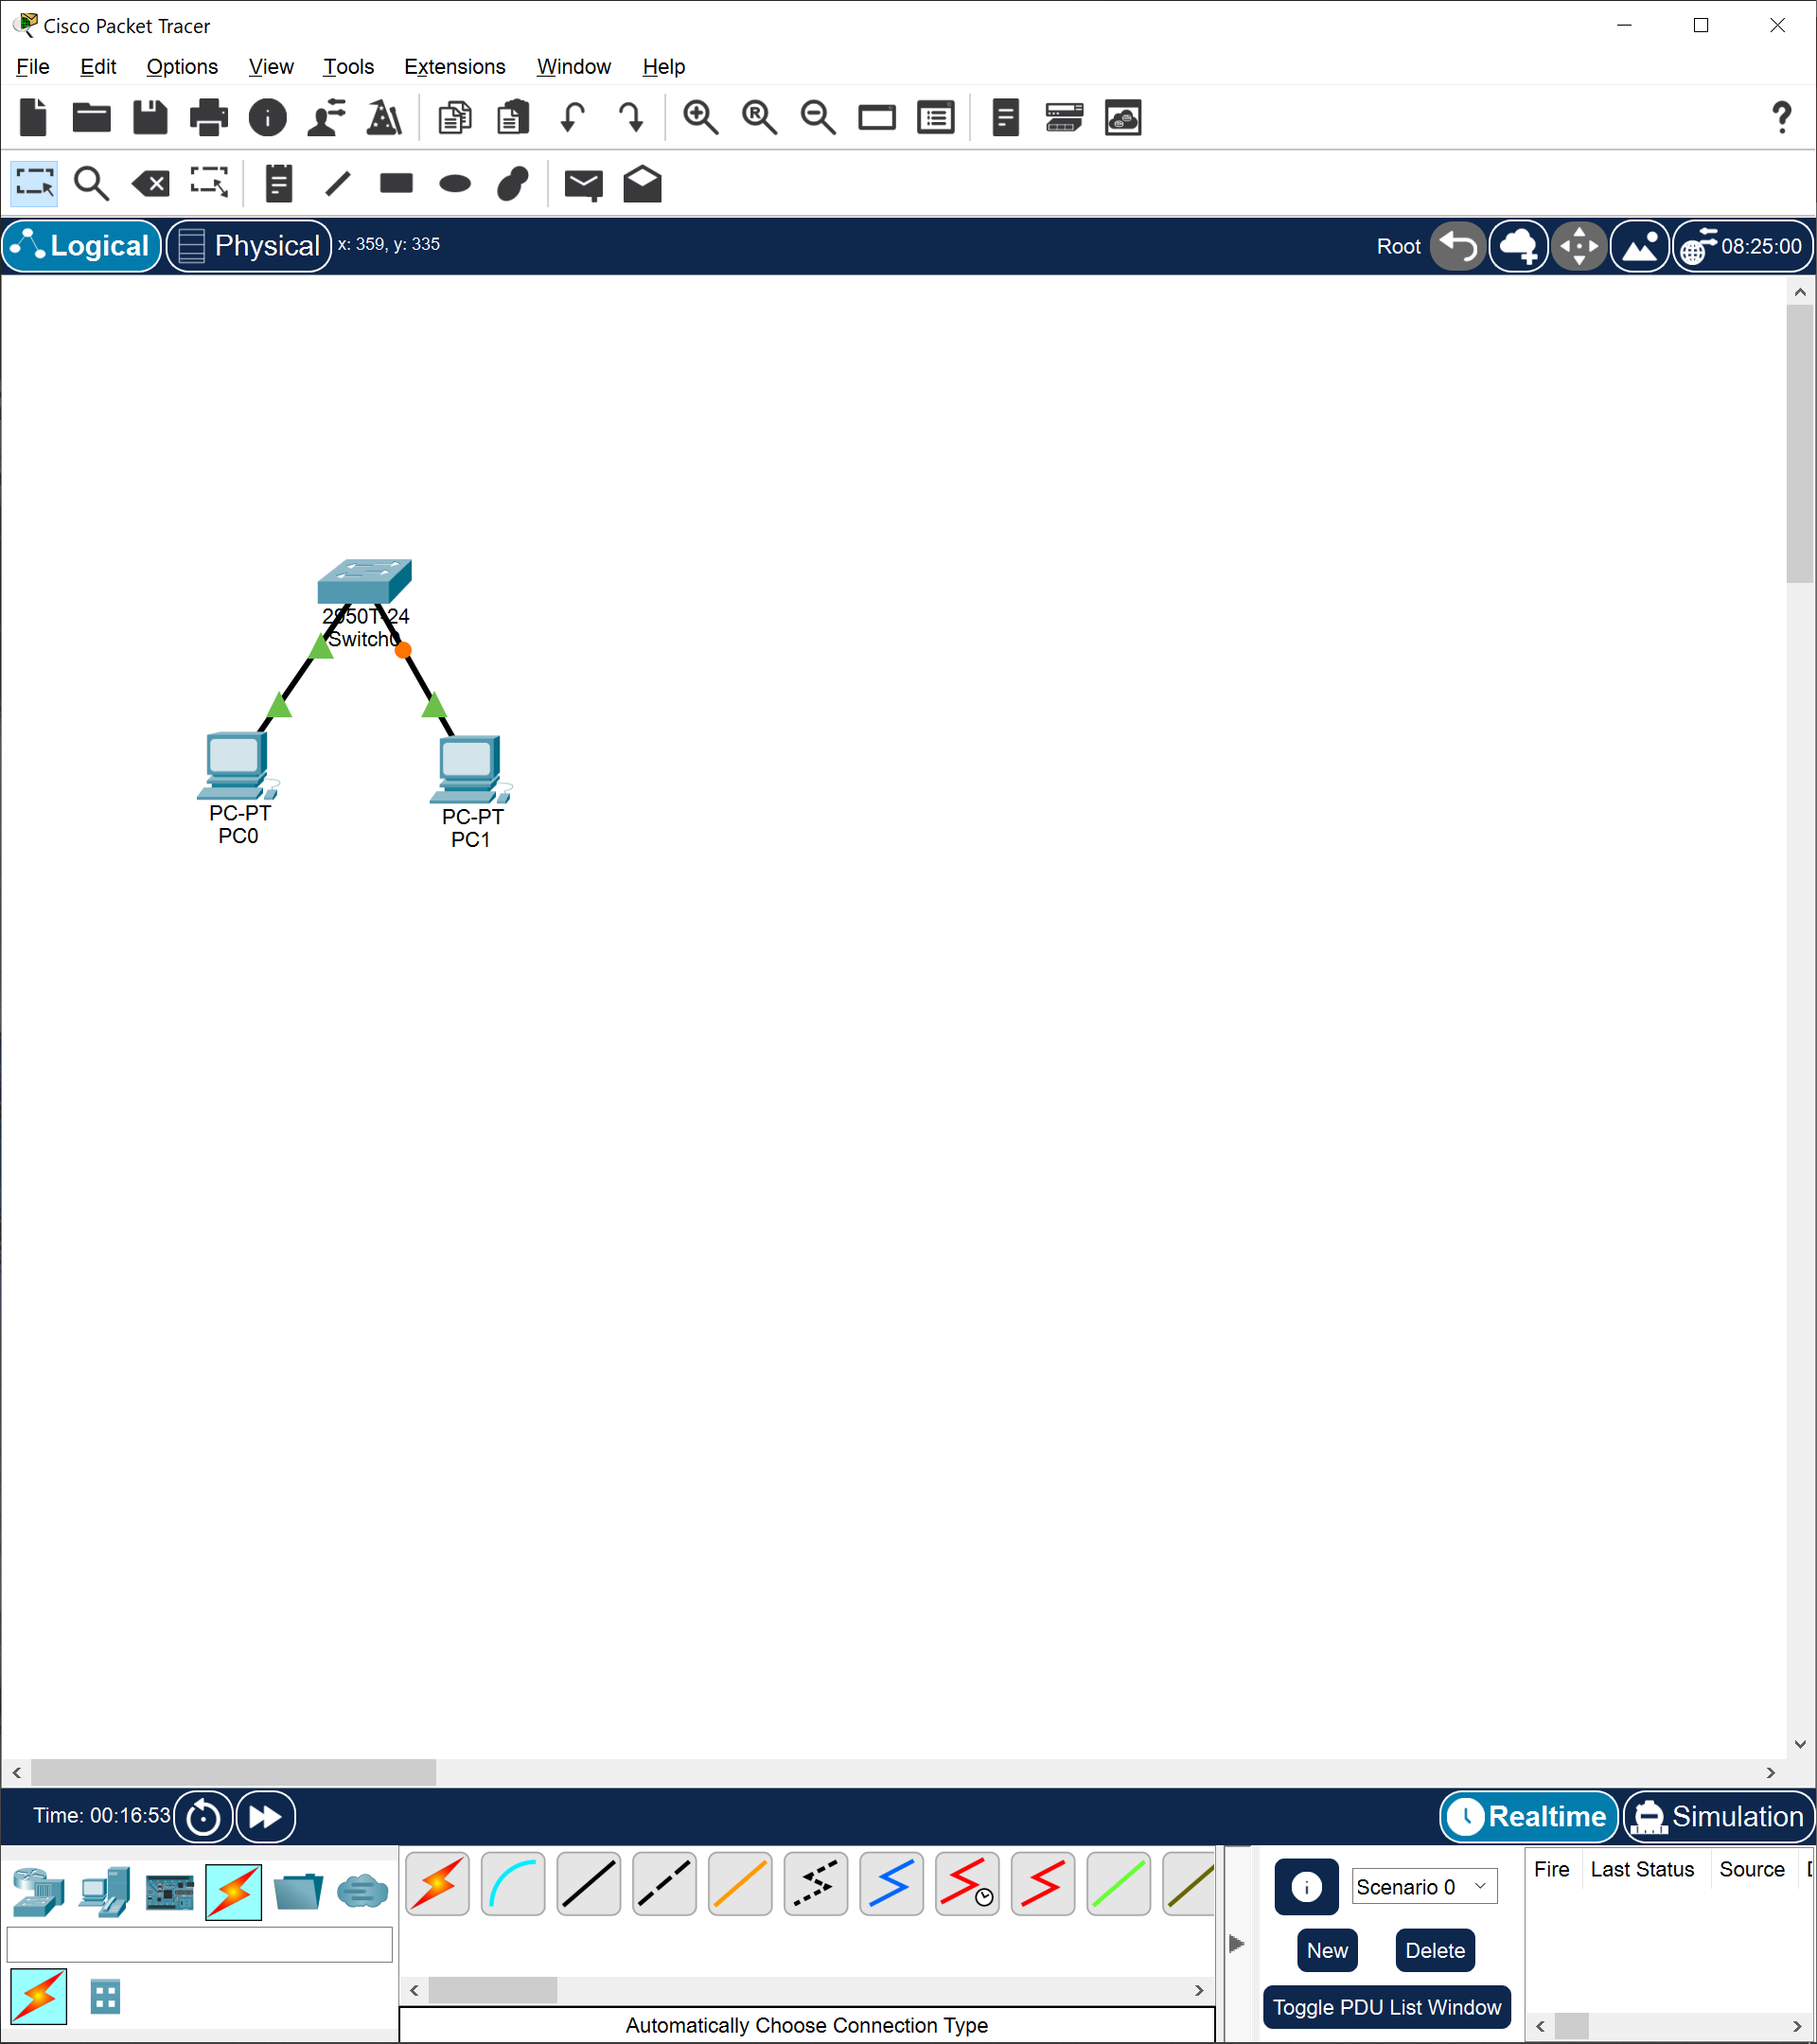
\includegraphics[width=13cm]{./step-by-step/9.PNG}
\clearpage

\noindent Now it's all green which makes us happy \newline

\noindent 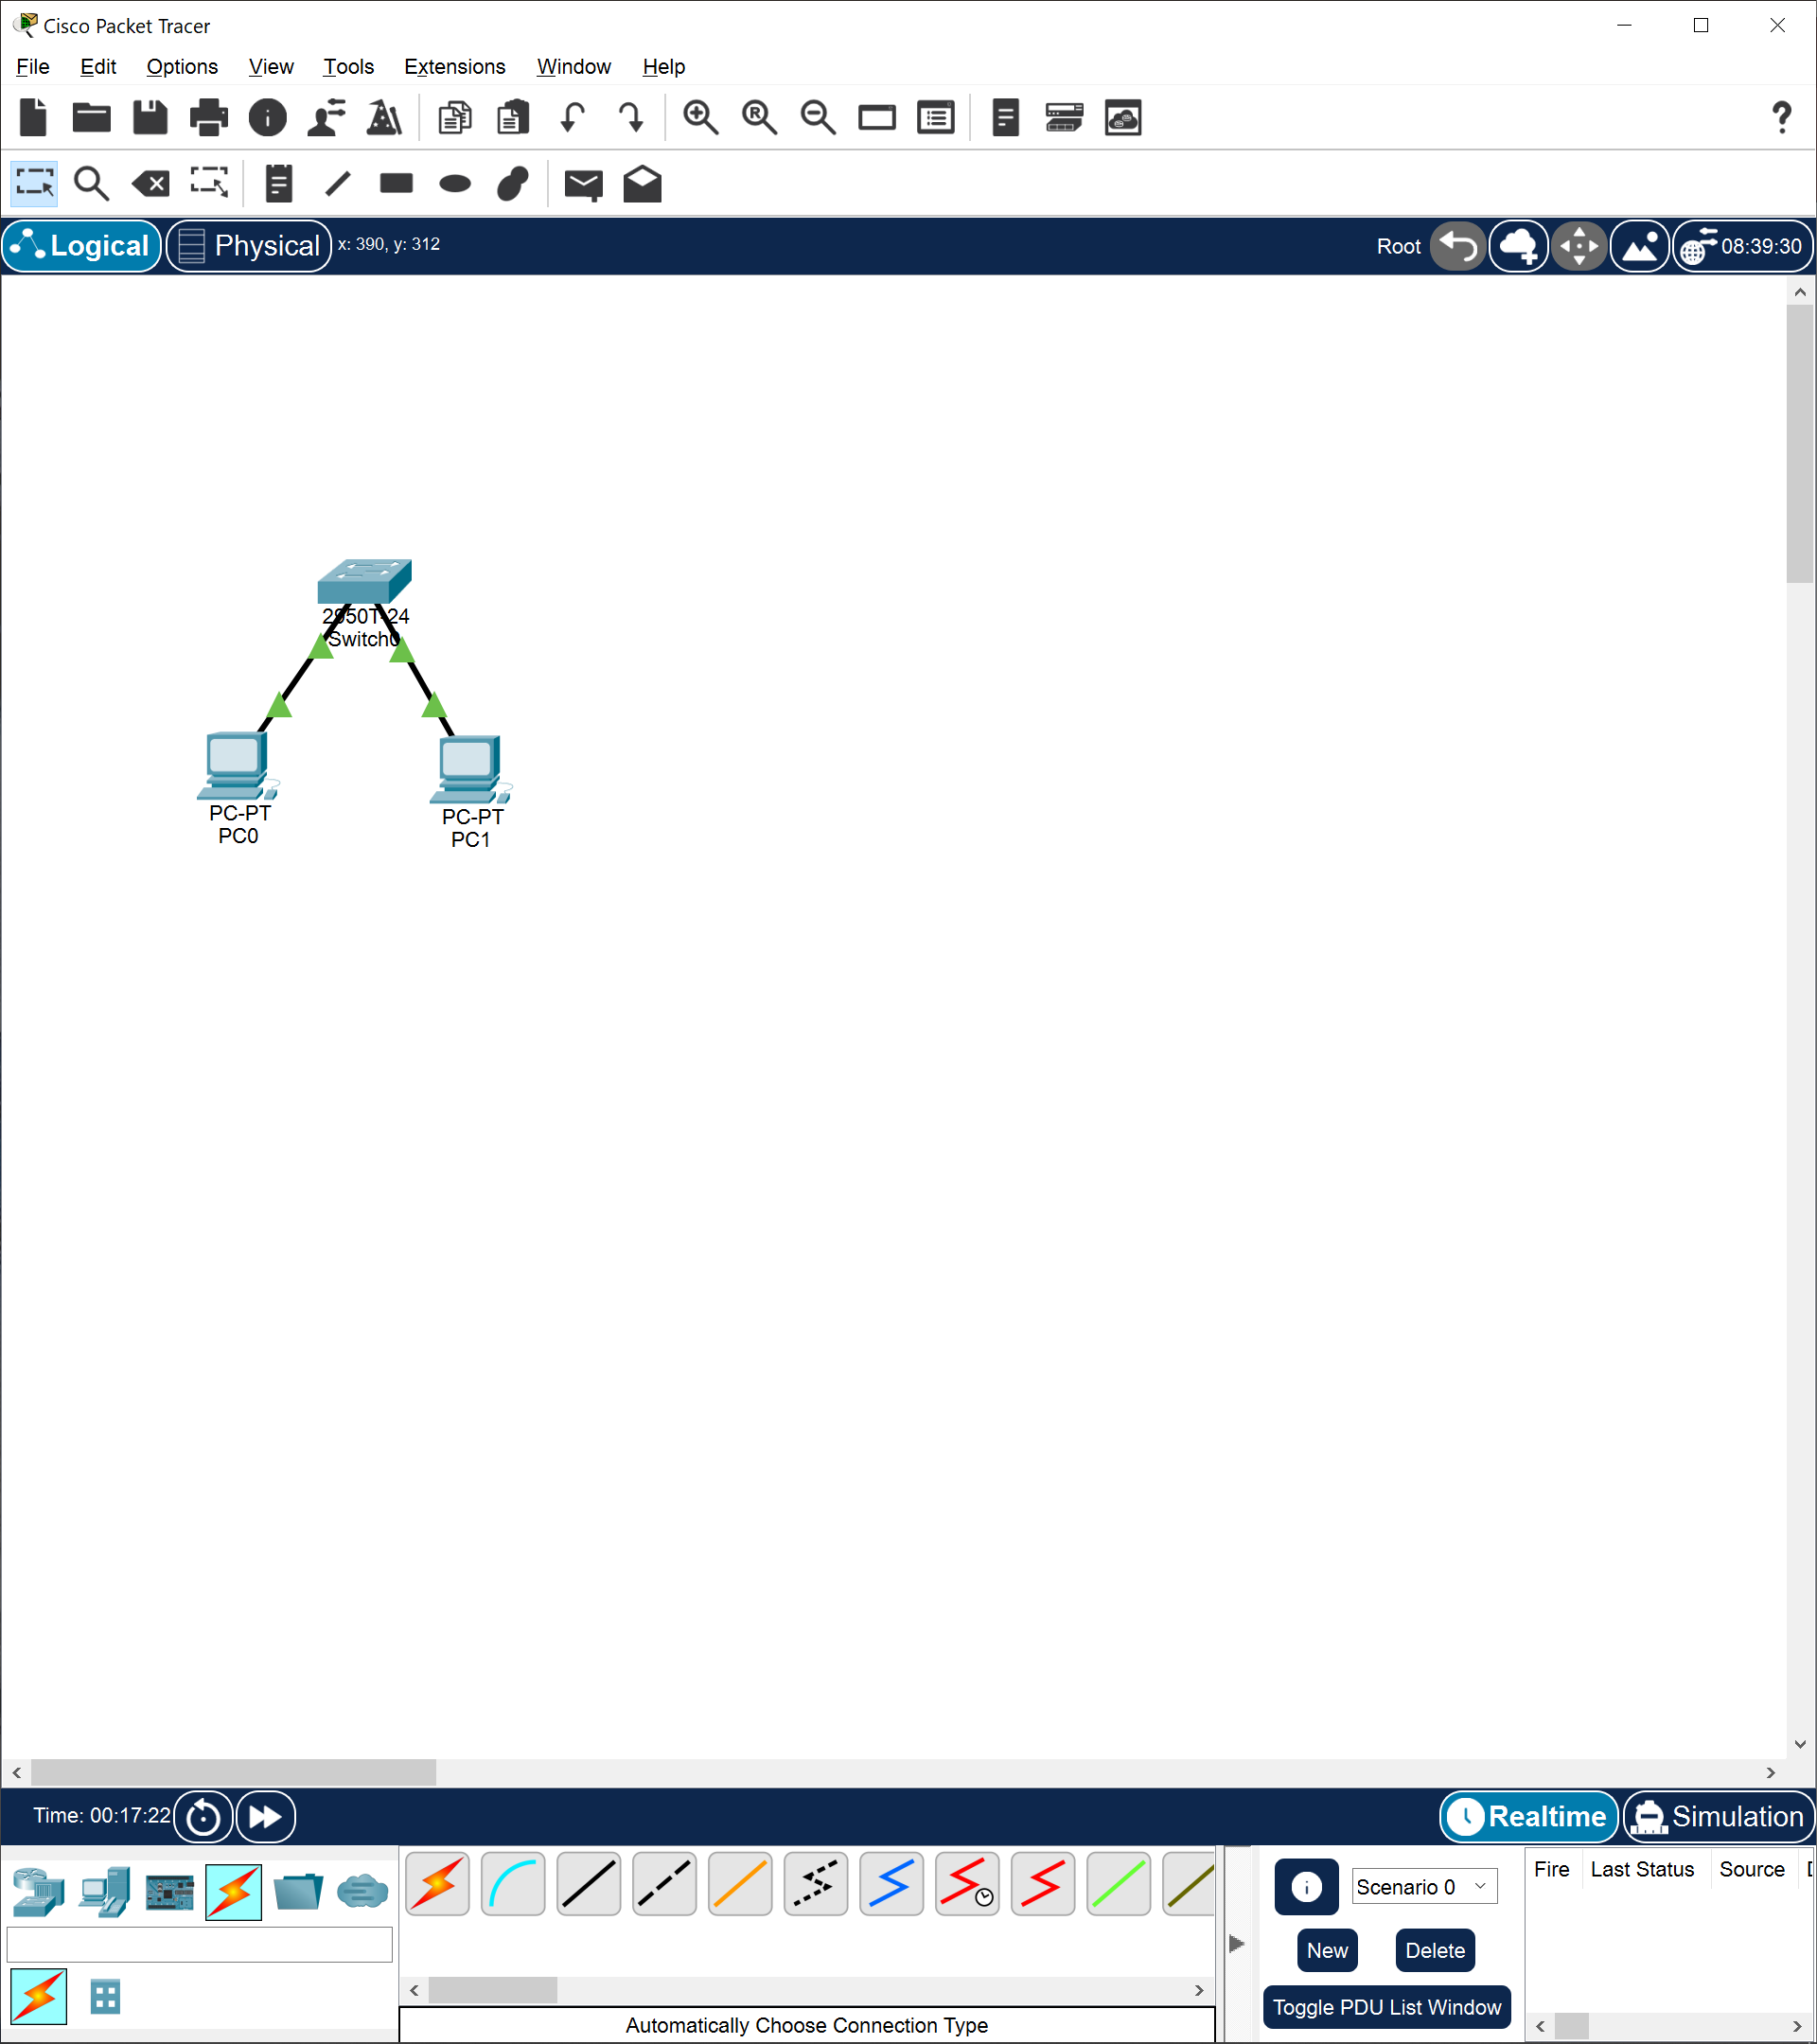
\includegraphics[width=13cm]{./step-by-step/10.PNG}
\clearpage

\noindent Let's add a router \newline

\noindent 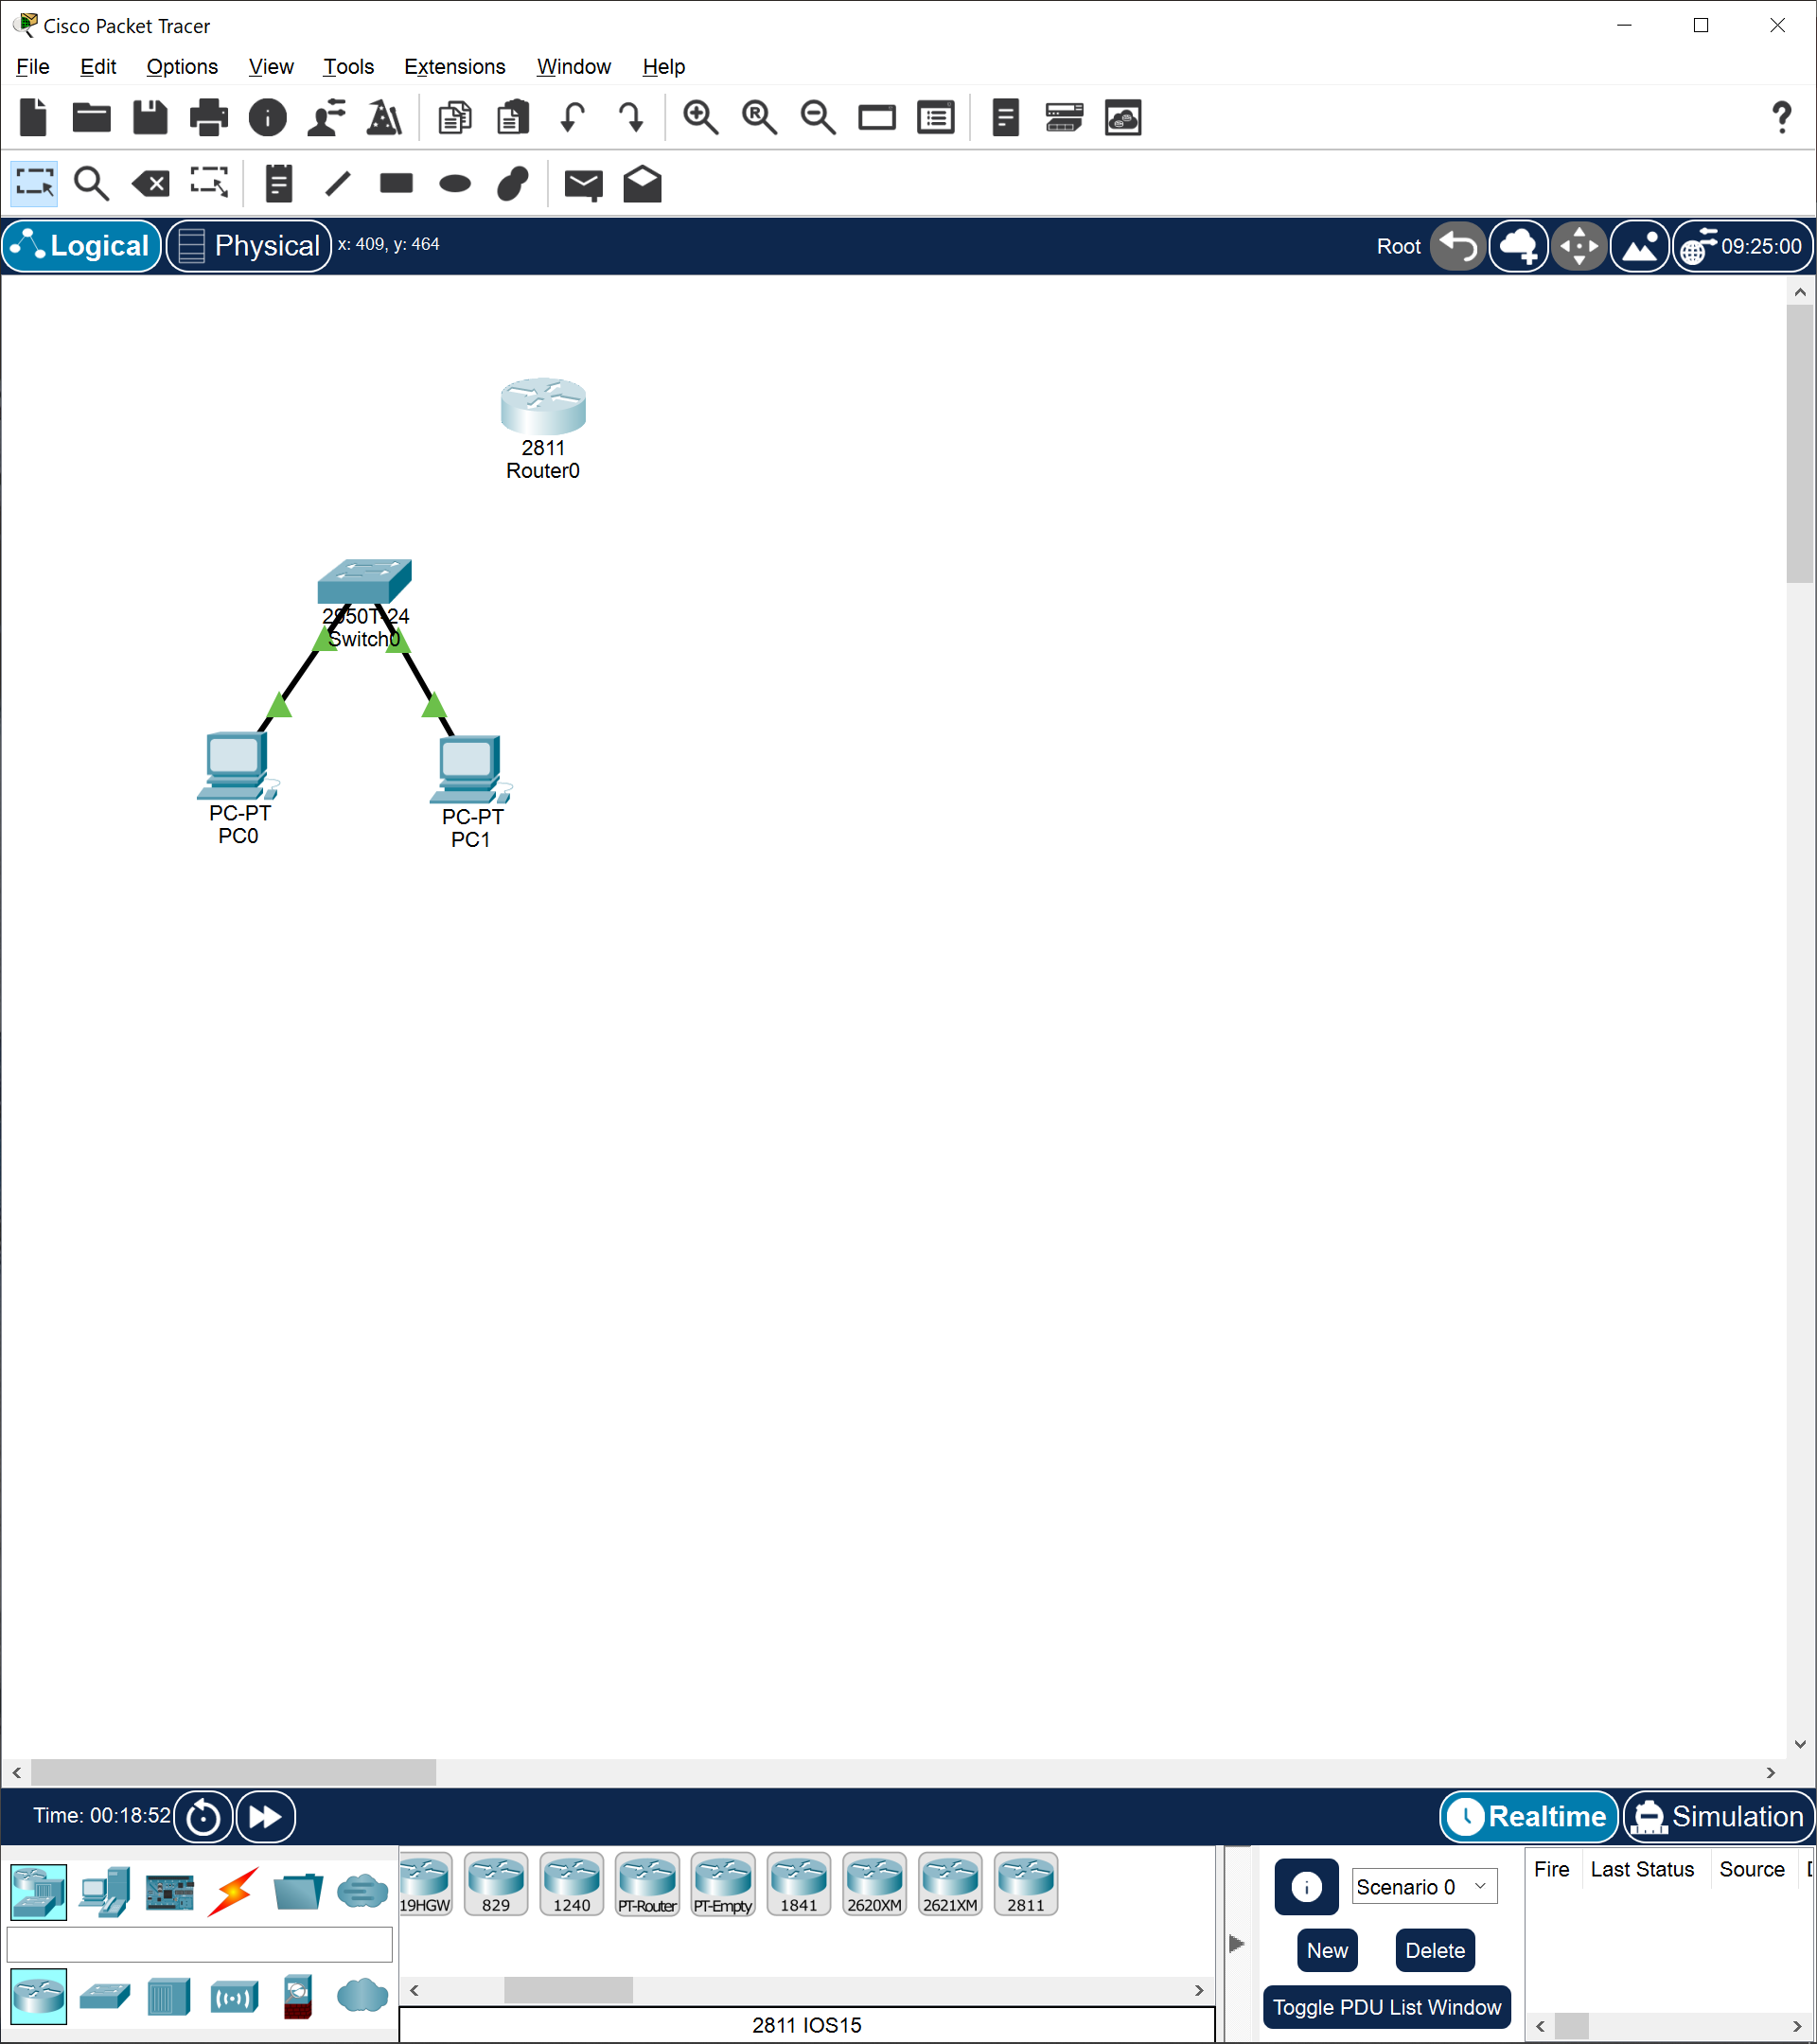
\includegraphics[width=13cm]{./step-by-step/11.PNG}
\clearpage

\noindent Let's link the router to the first computer \newline

\noindent 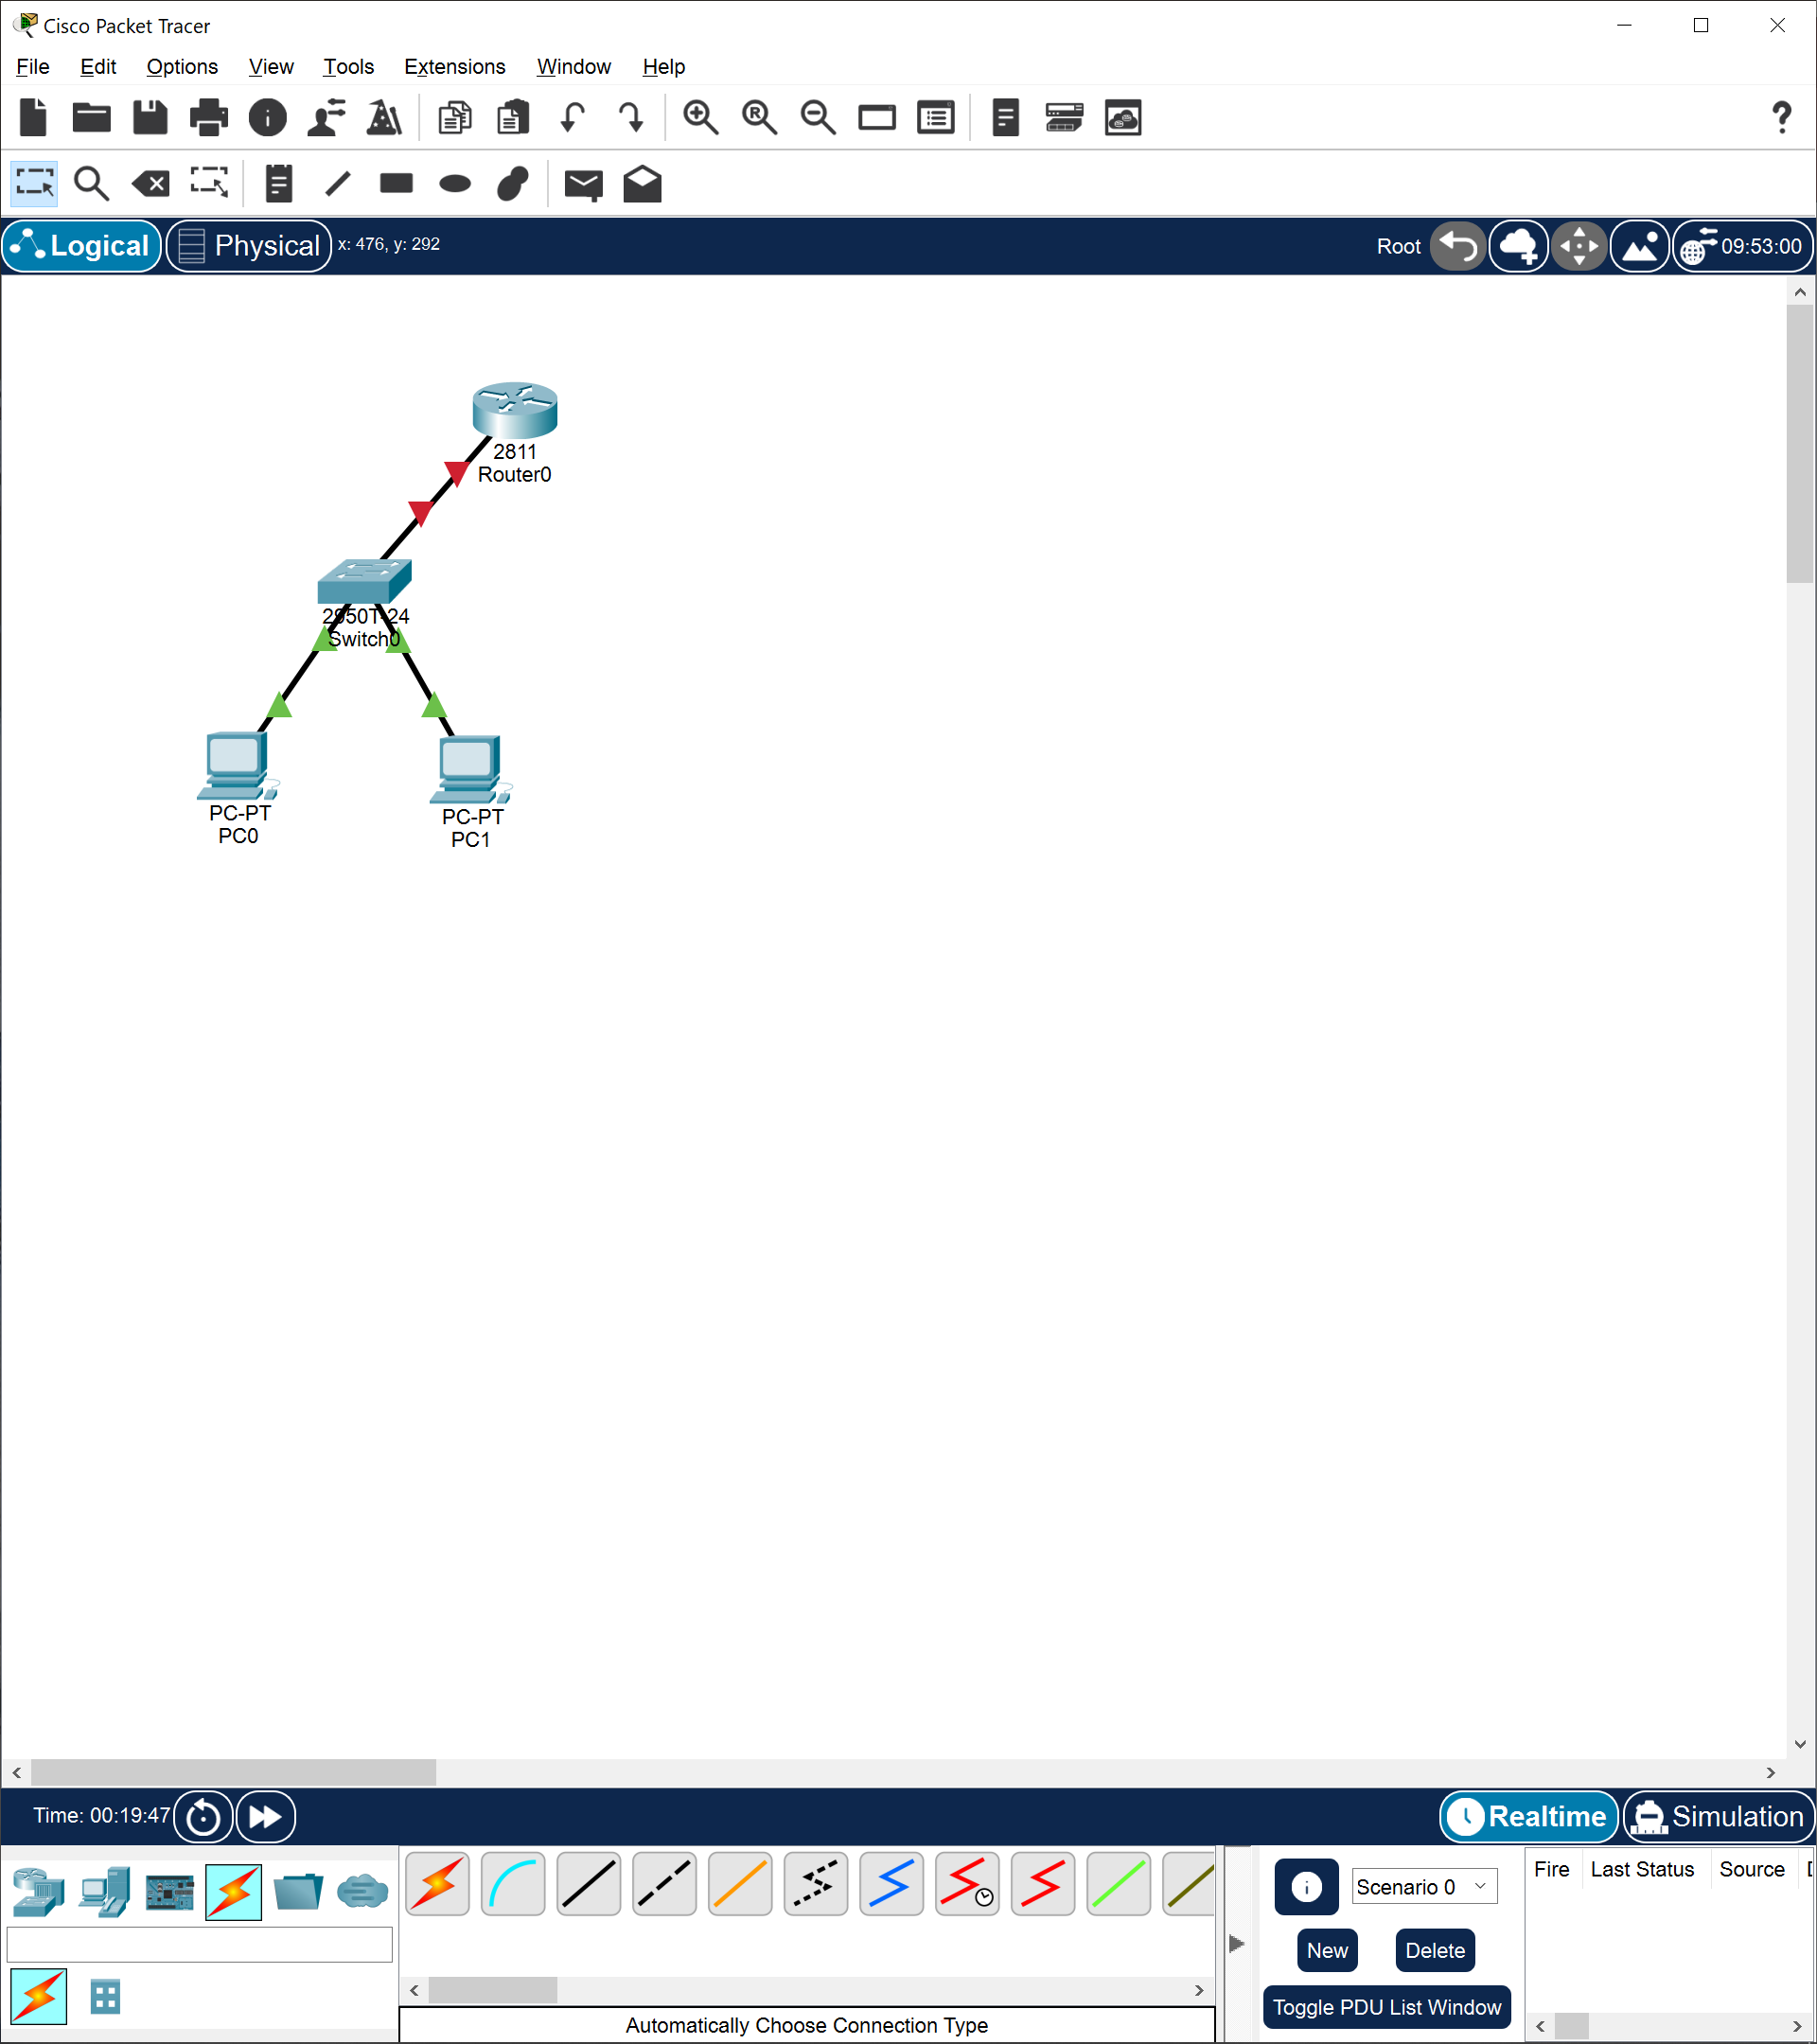
\includegraphics[width=13cm]{./step-by-step/12.PNG}
\clearpage

\noindent If you click on the router, in the config tab there is a box you need to check. That box will emulate the router being powered on \newline

\noindent 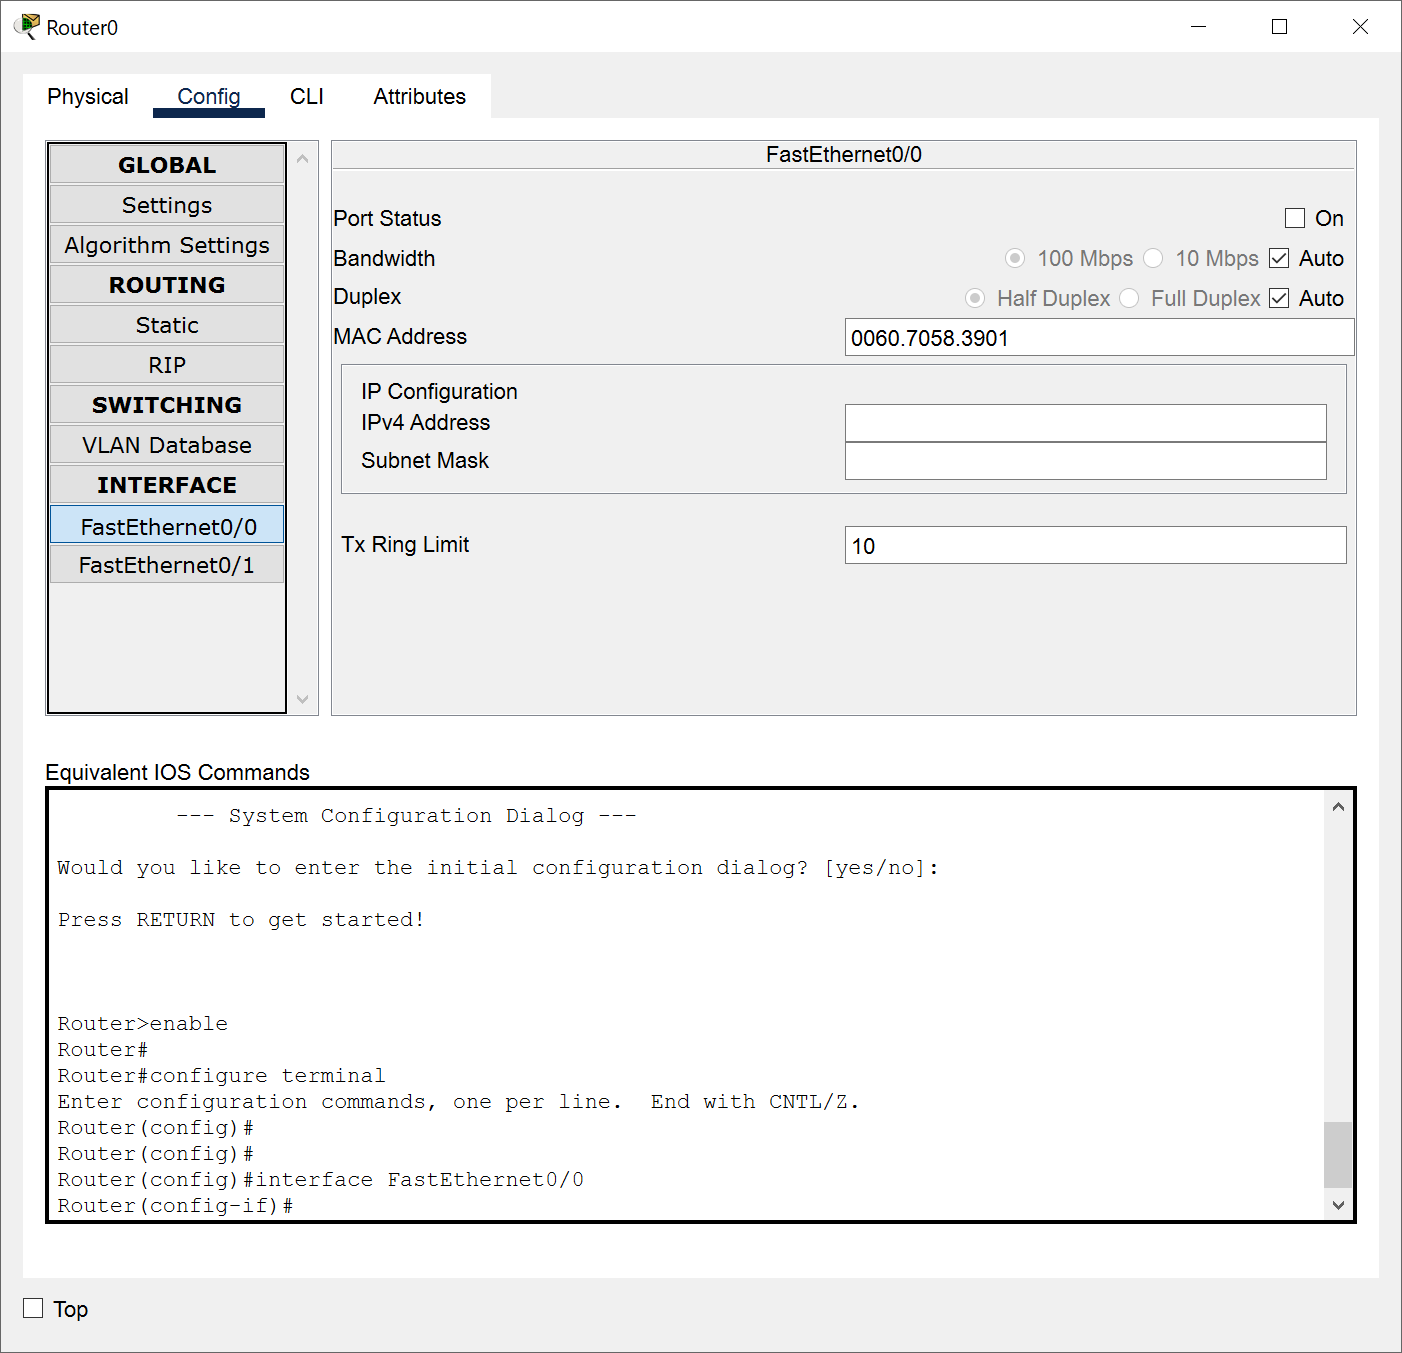
\includegraphics[width=13cm]{./step-by-step/13.PNG}
\clearpage


\noindent Once you click in the box a small tick will appear in it. This means the box is ticked and the function that box is proving is now being turned on \newline

\noindent 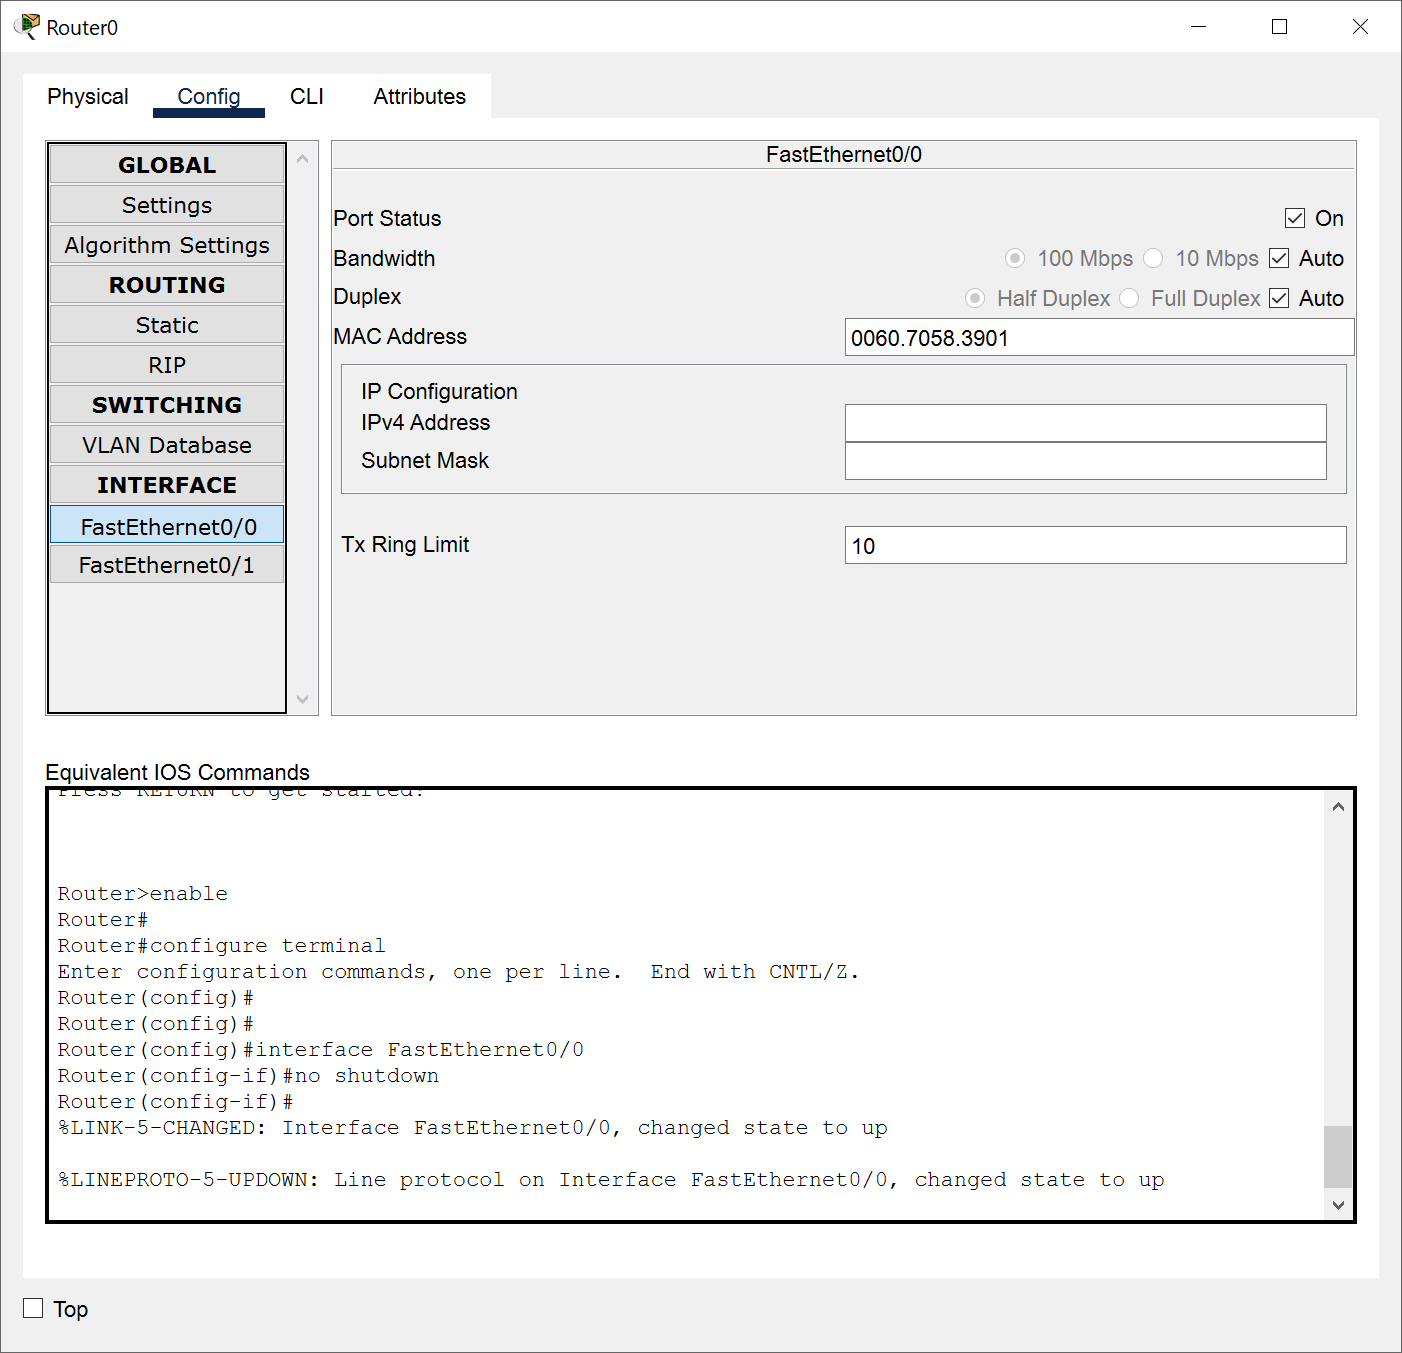
\includegraphics[width=13cm]{./step-by-step/14.PNG}
\clearpage

\noindent as a result of ticking that box now you can see the link going green wich means is enabled for data transmission \newline

\noindent 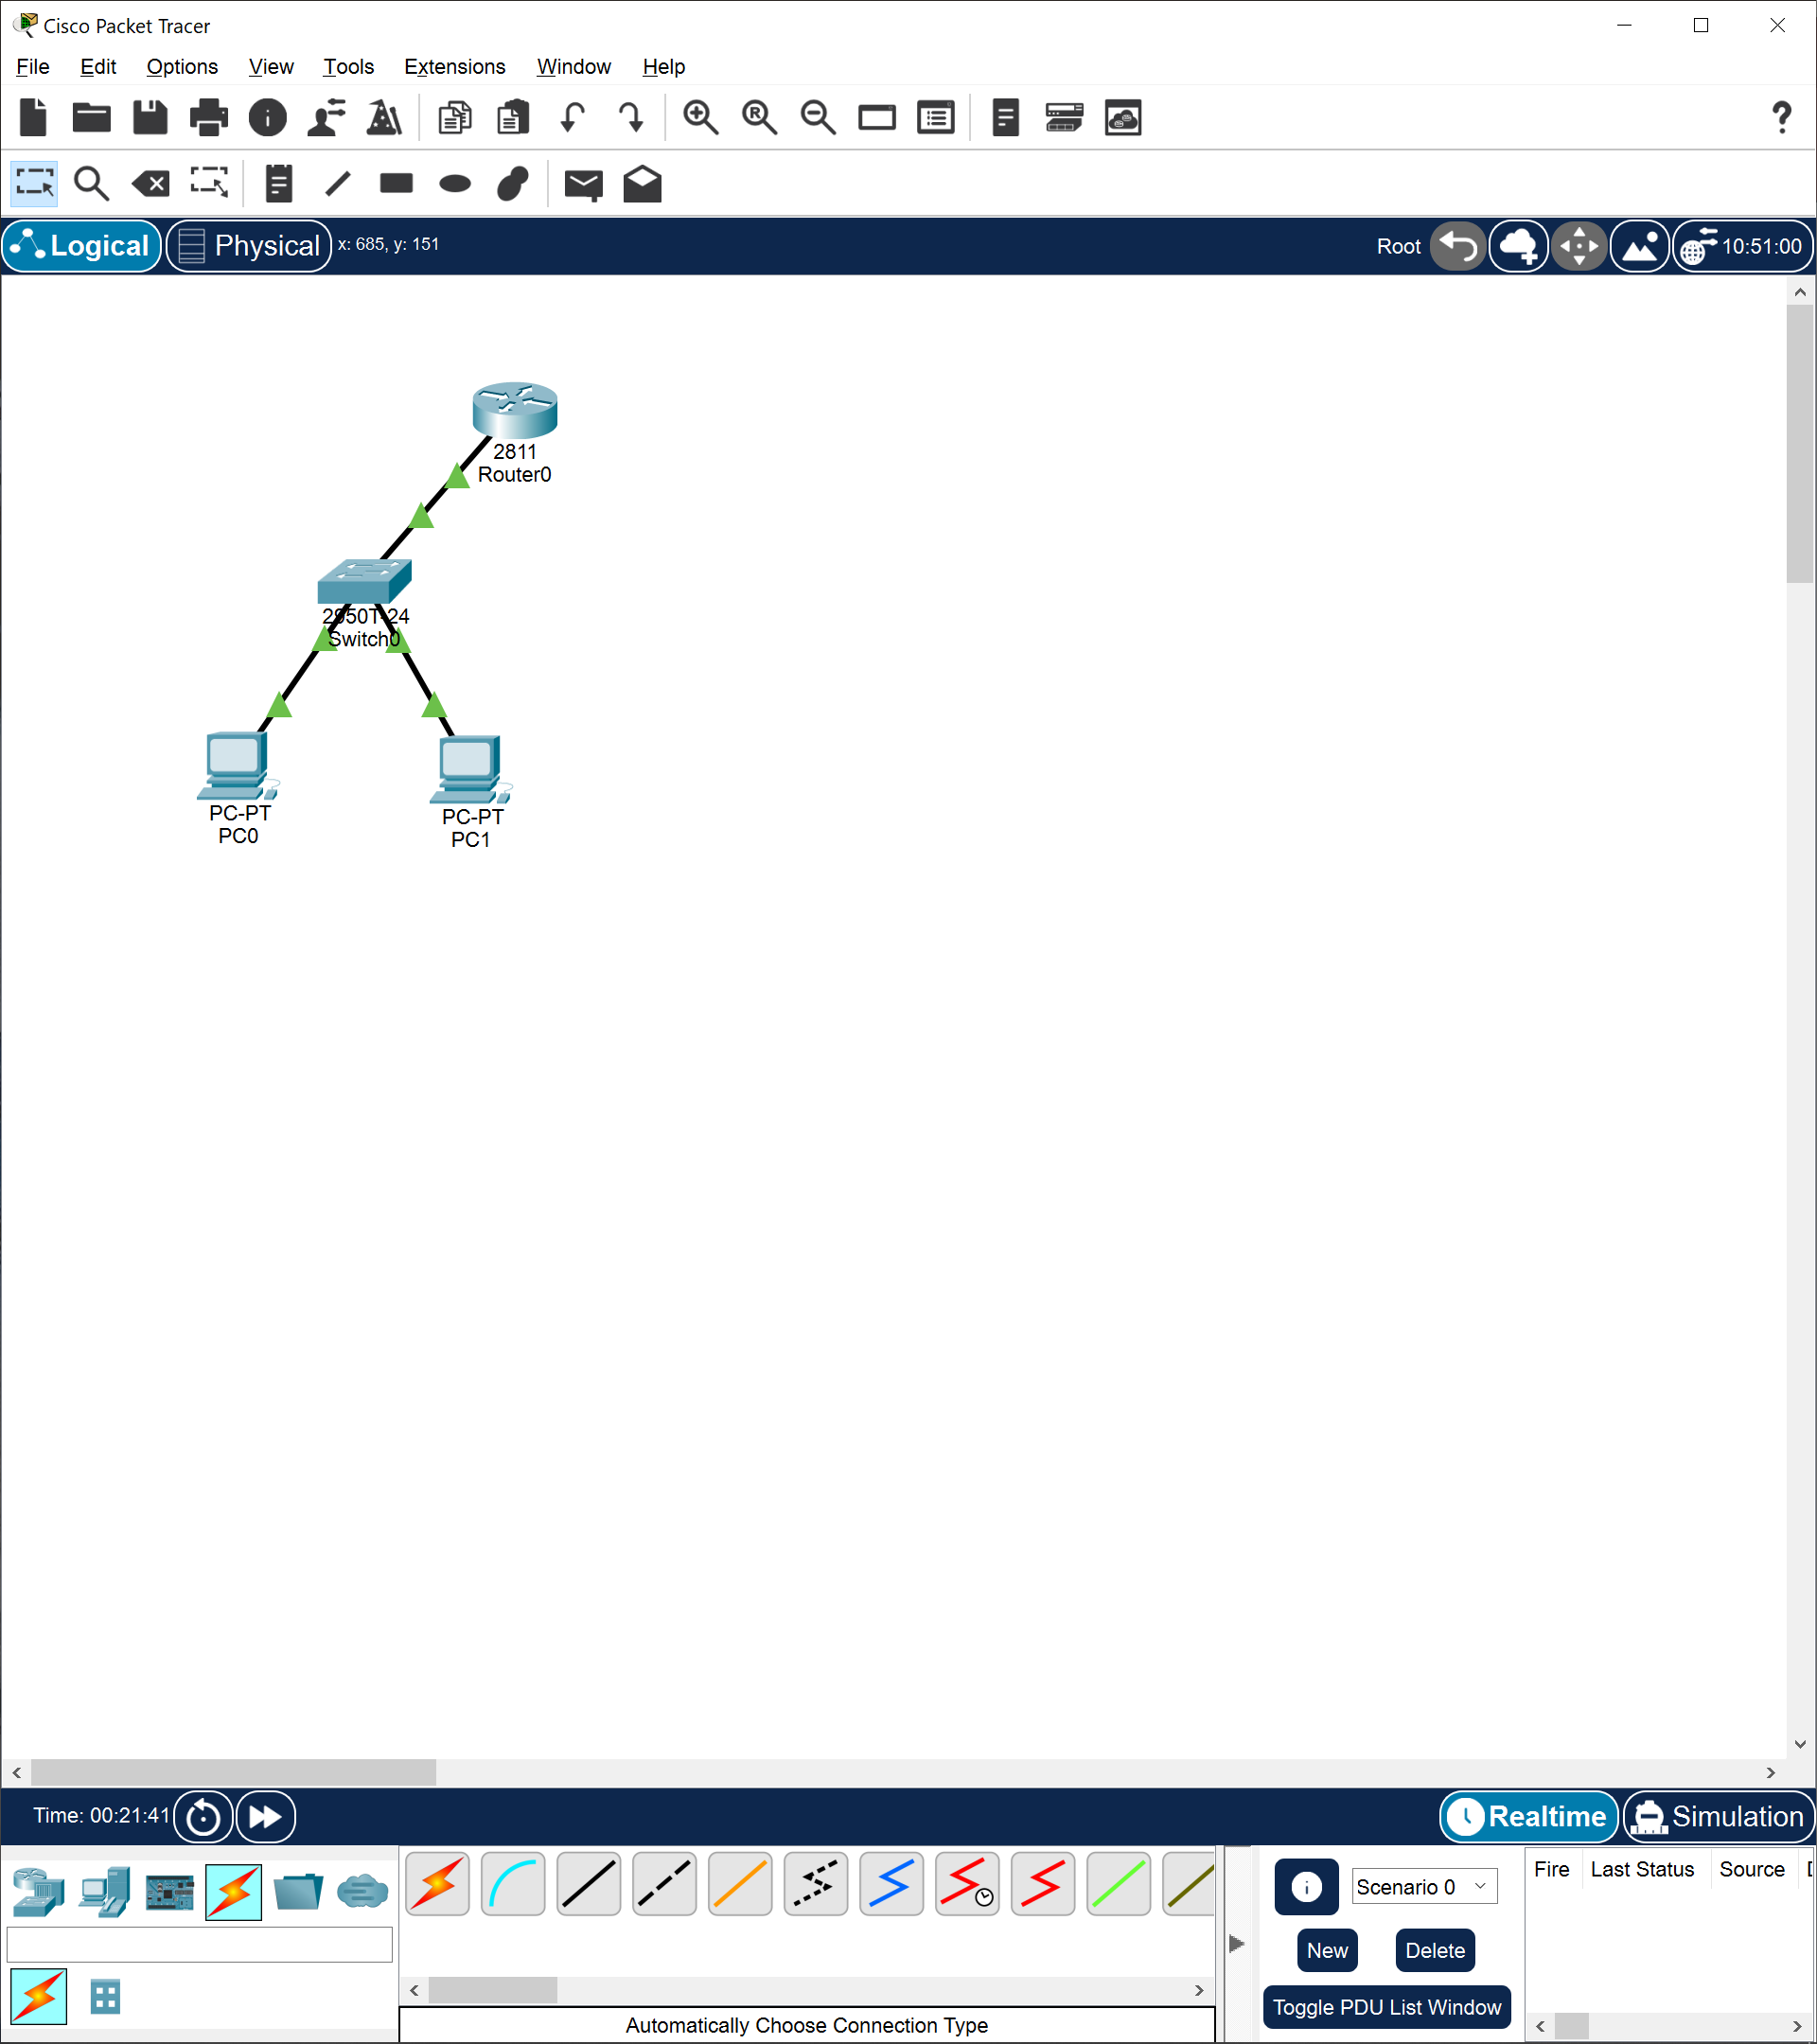
\includegraphics[width=13cm]{./step-by-step/15.PNG}
\clearpage


\noindent we only need to sort the \textbf{IP Configuration} out as well \newline

\noindent 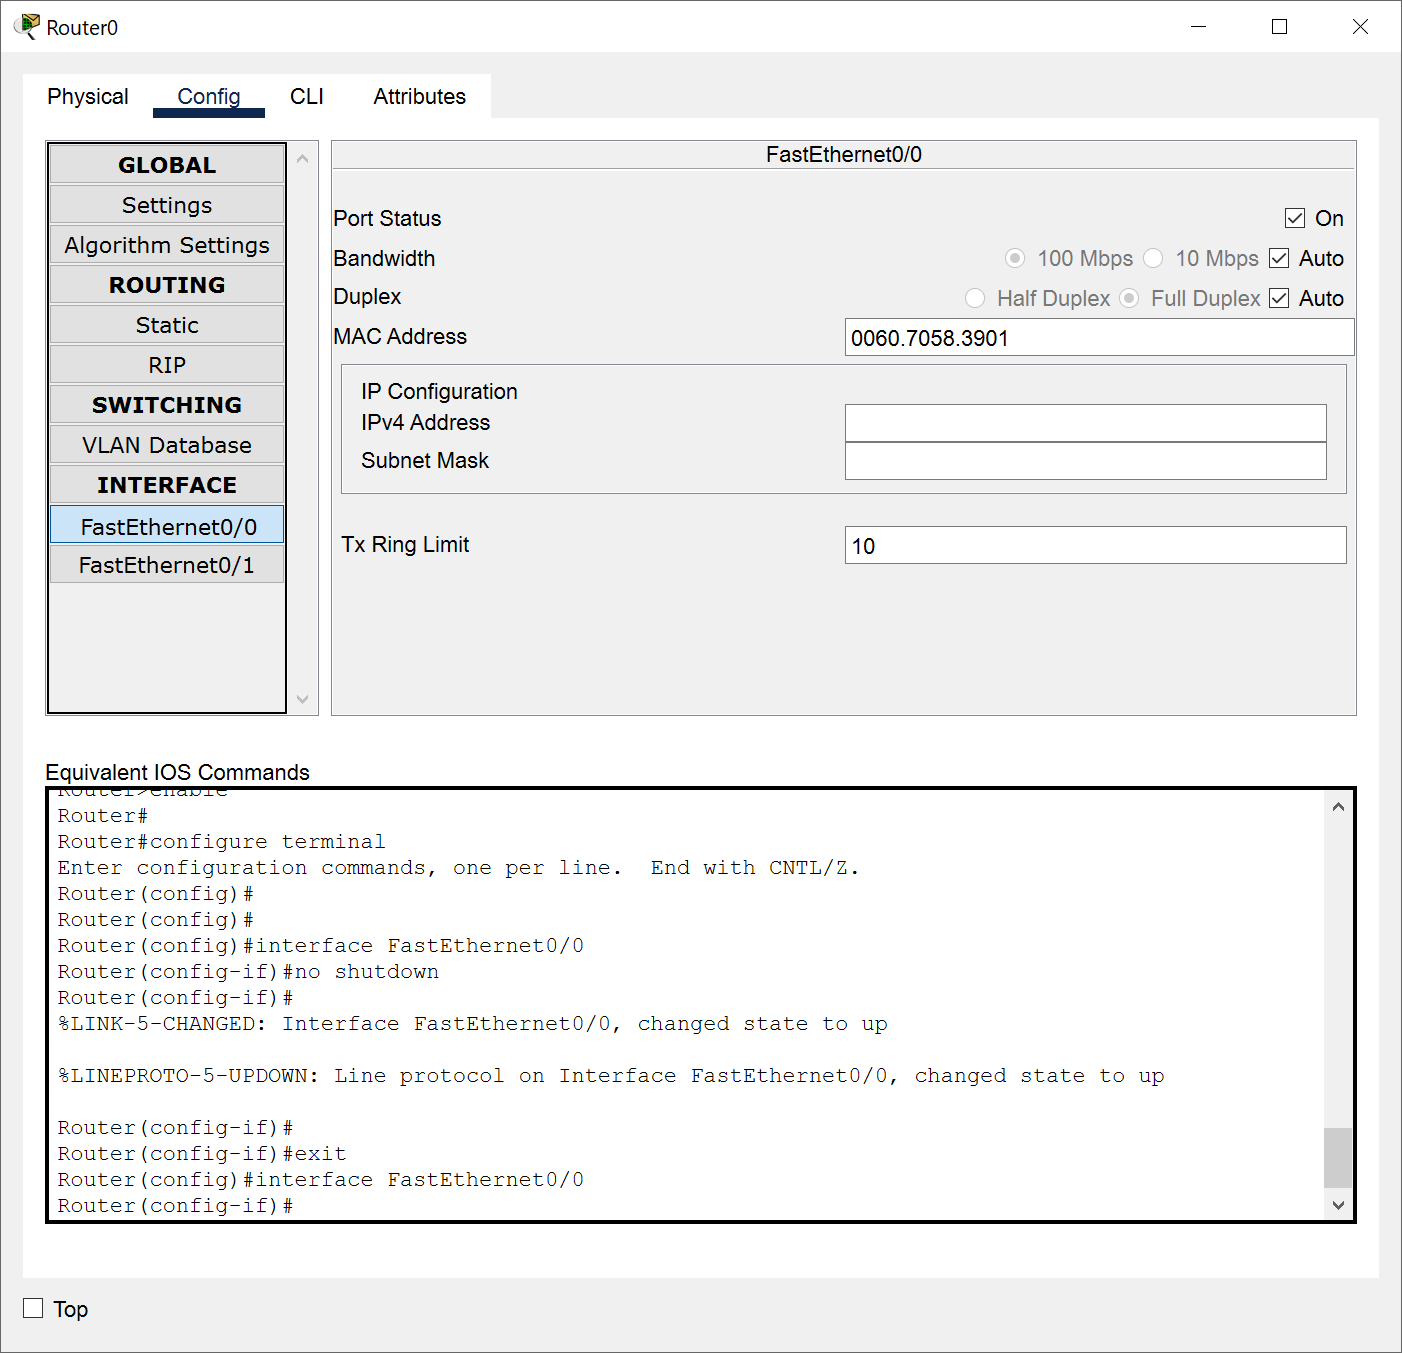
\includegraphics[width=13cm]{./step-by-step/16.PNG}
\clearpage


\noindent Now, because the subnet mask indicates how many values can you actually use this means we can use

\[ 255 values - X values \]

\noindent where \emph{X} is the number in a subnetmask like \emph{Z.Y.W.X} which in the case of \emph{255.255.255.0} will be

\[ 255 - 0\]

\noindent which returns 255 values but because we start counting from 0 we can go up to 254.
In the following example you can see the value 0 being accepted as a valid value \newline 

\noindent 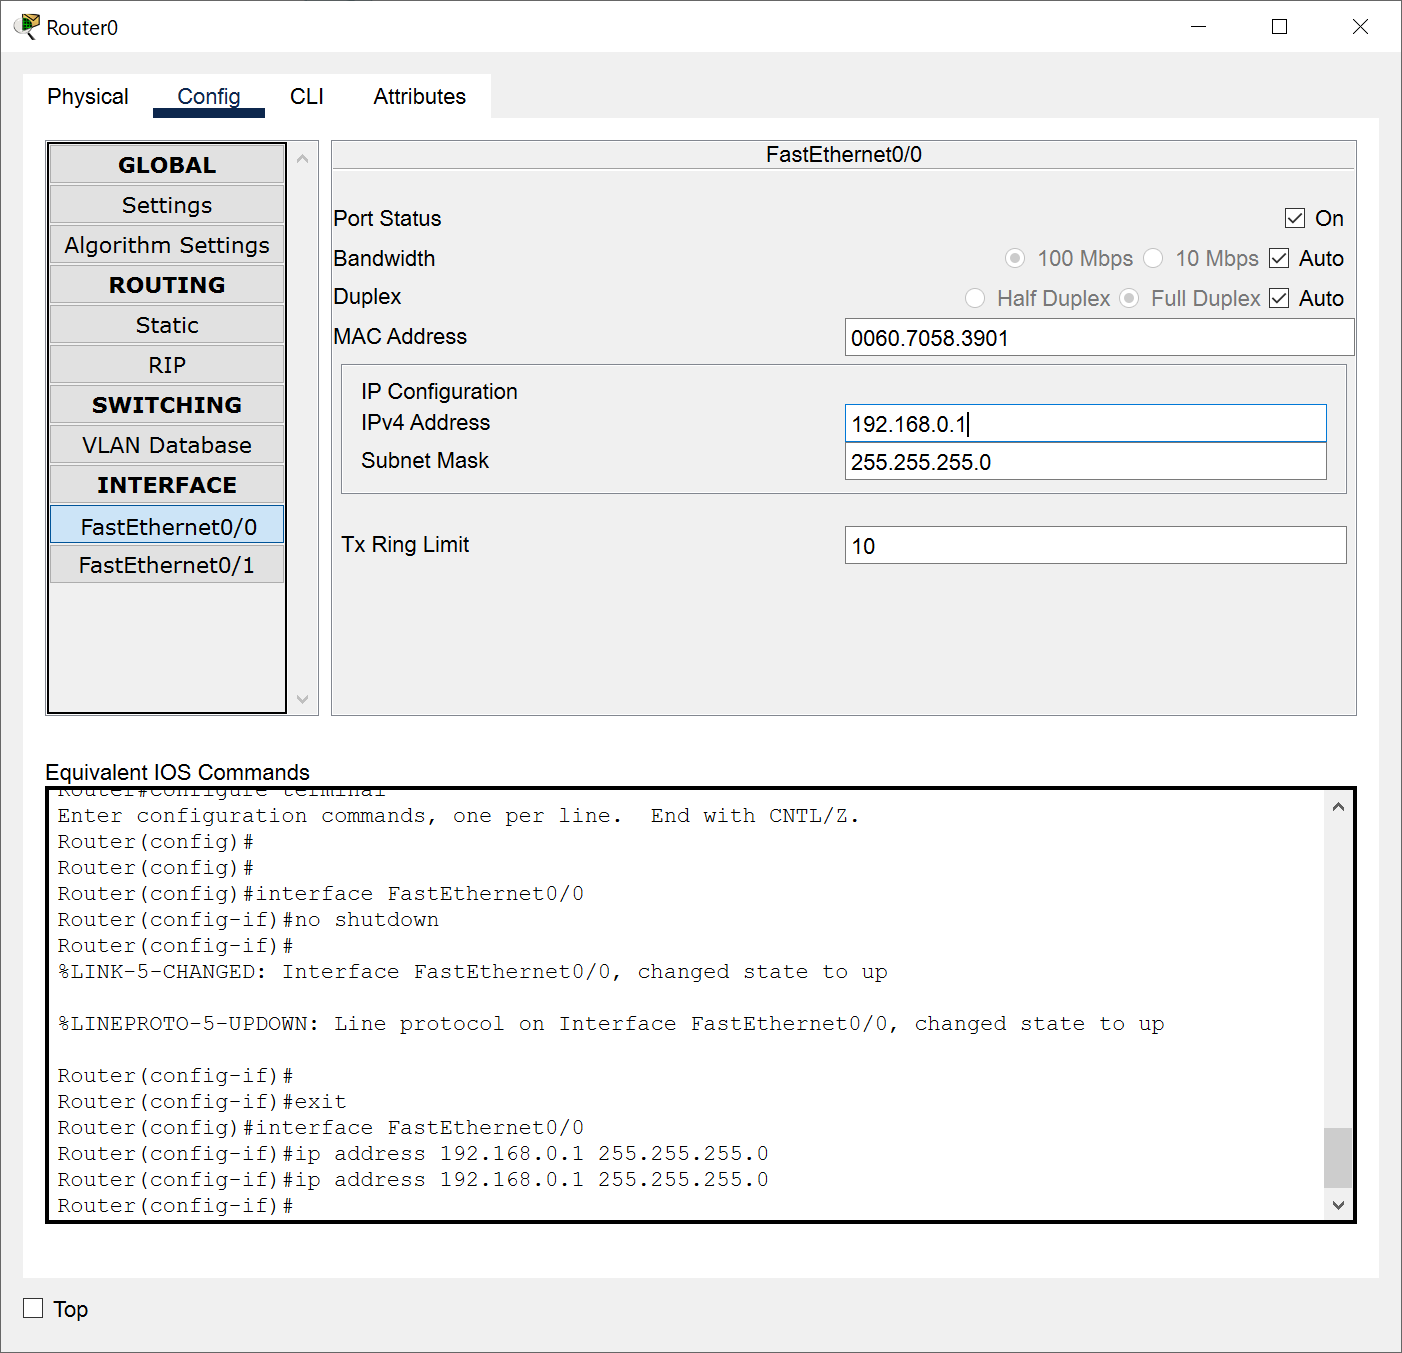
\includegraphics[width=13cm]{./step-by-step/17.PNG}
\clearpage


\noindent Let's pick up PC1 console and ping all devices in the 192.168.0.1 network. The ping works \newline

\noindent 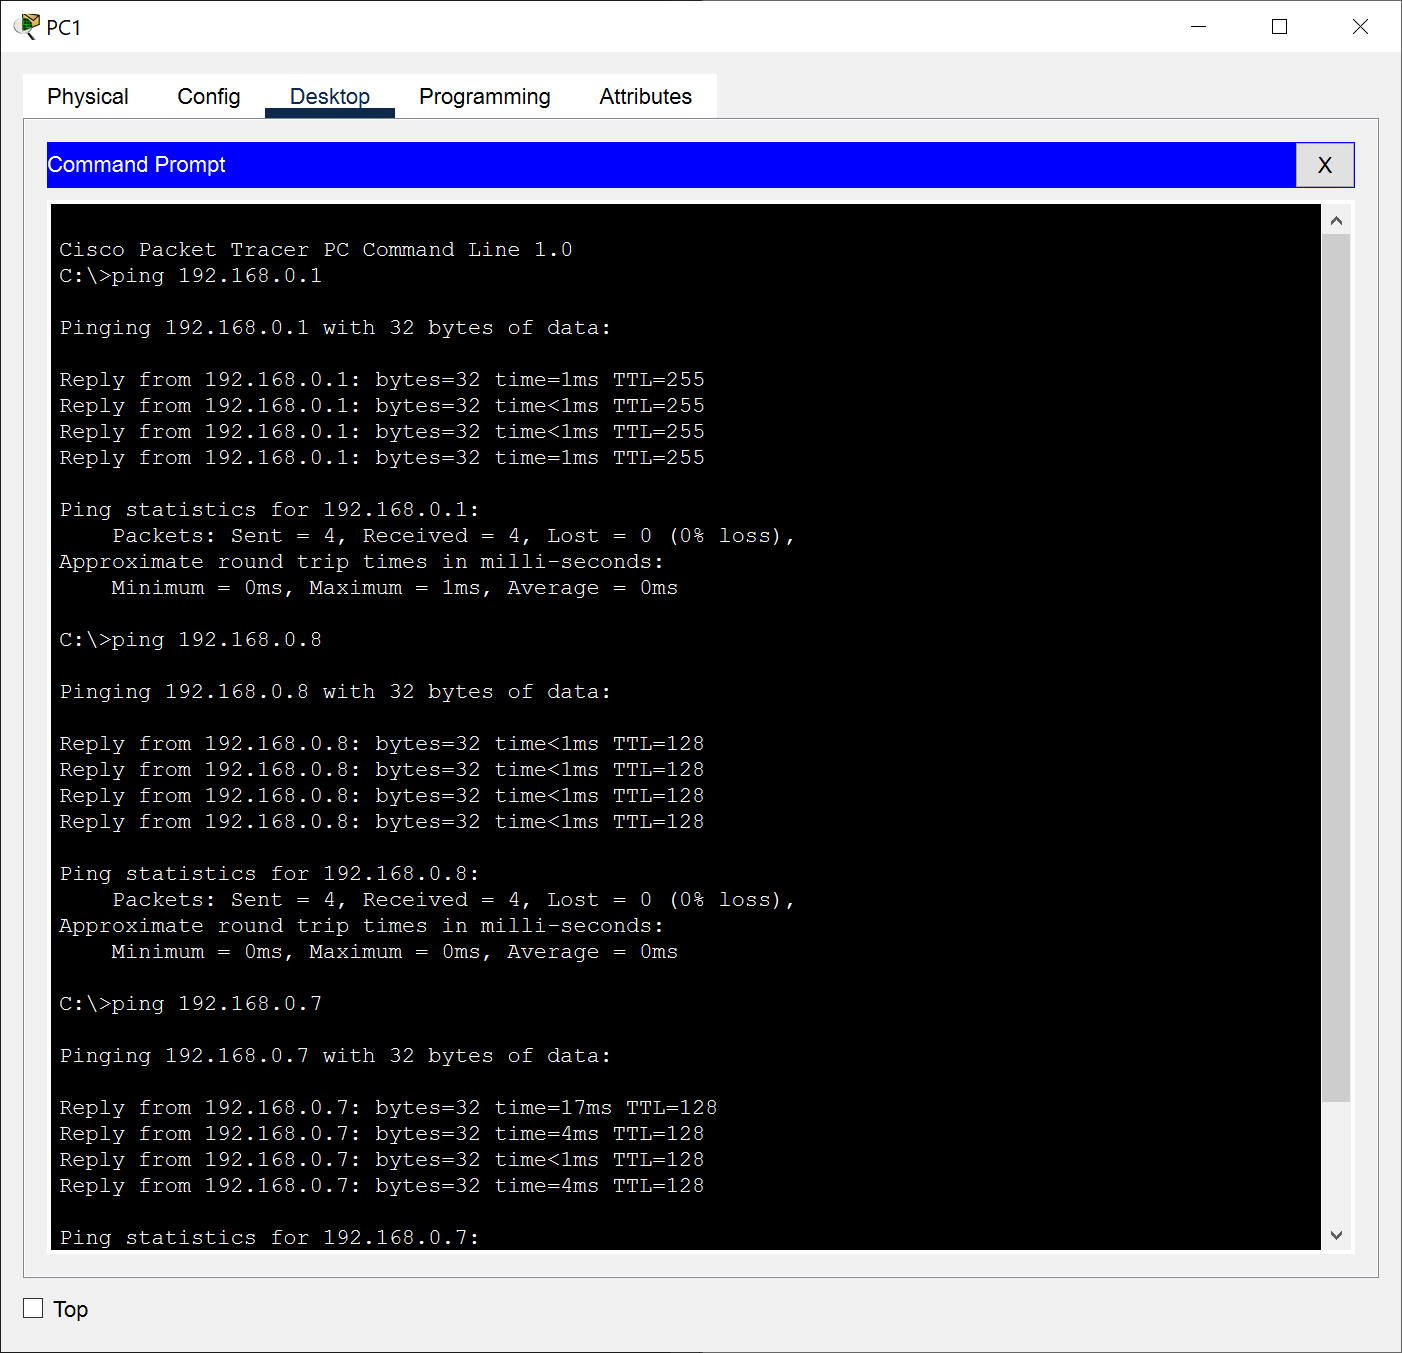
\includegraphics[width=13cm]{./step-by-step/18.PNG}
\clearpage

\noindent Let's create a copy of the subnetwork we have already. The gateway will be this time 
\[192.168.1.1\] \newline
 
\noindent 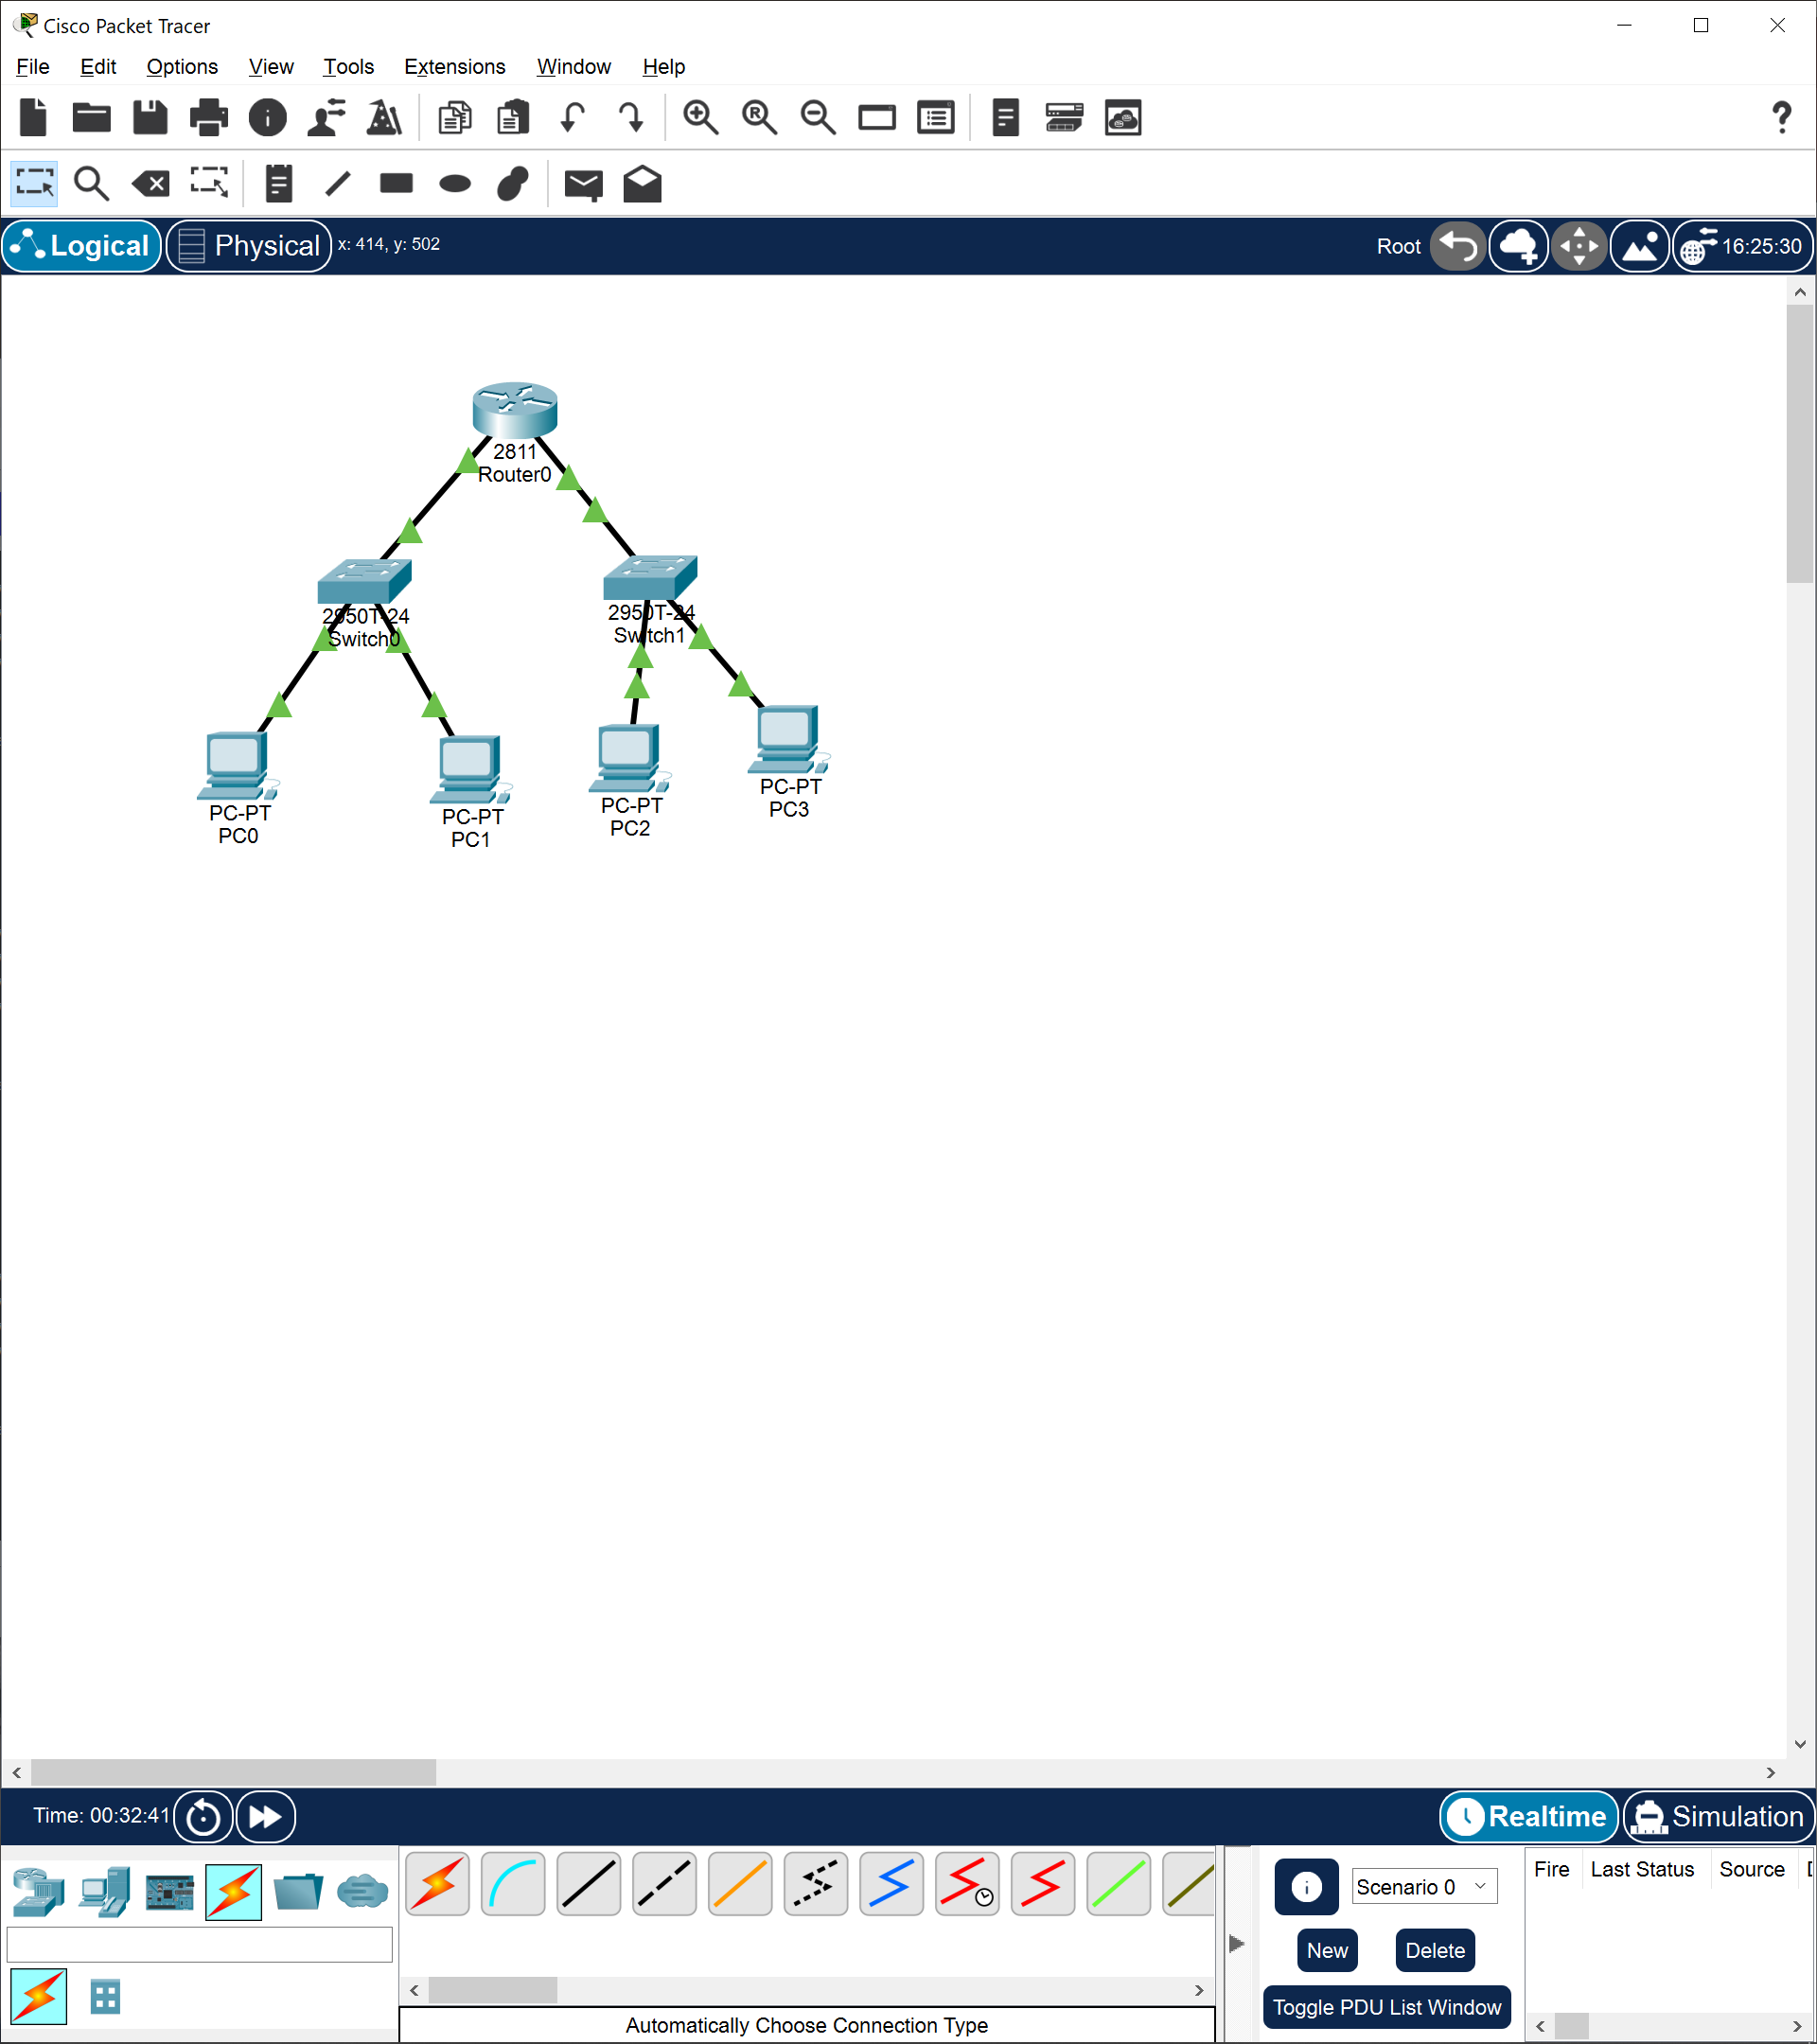
\includegraphics[width=13cm]{./step-by-step/19.PNG}
\clearpage

\subsubsection{expanding the network}
\noindent Let's add a printer with the following IP
\[192.168.1.20\] \newline

\noindent 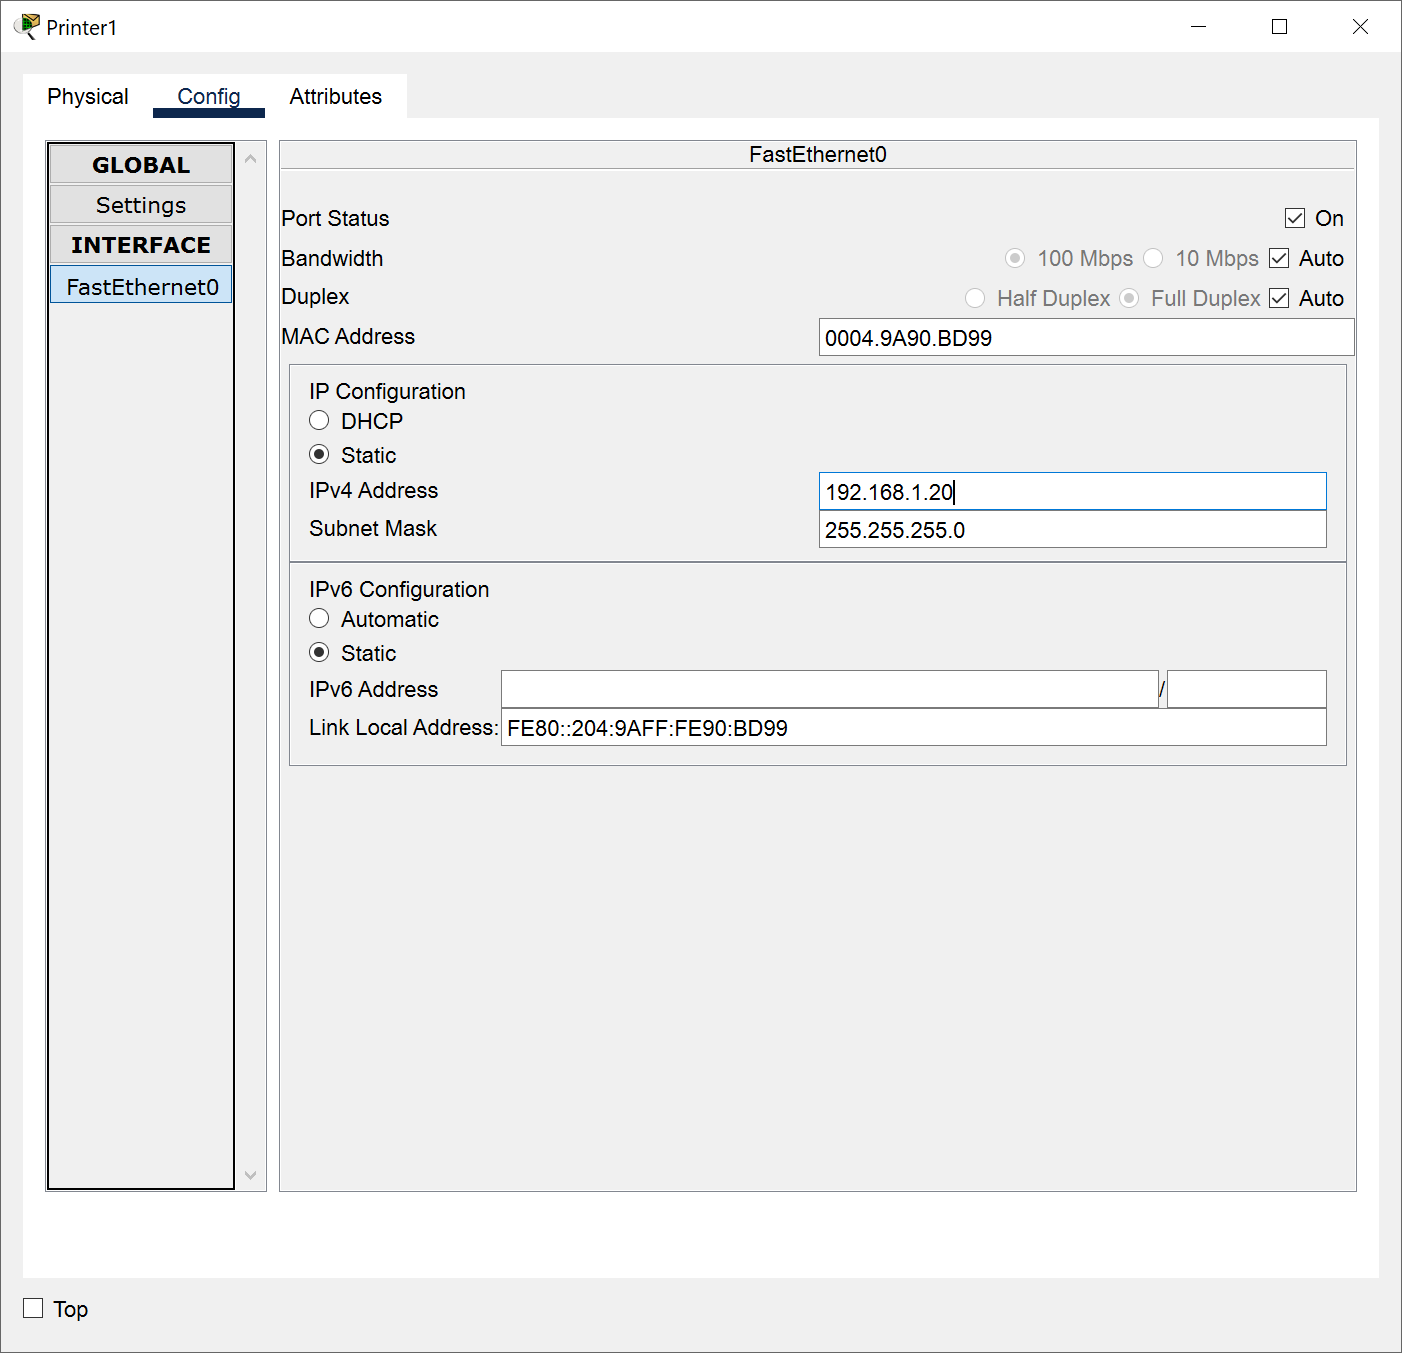
\includegraphics[width=13cm]{./step-by-step/20.PNG}
\clearpage

\noindent Let's ping the printer from PC0\newline

\noindent 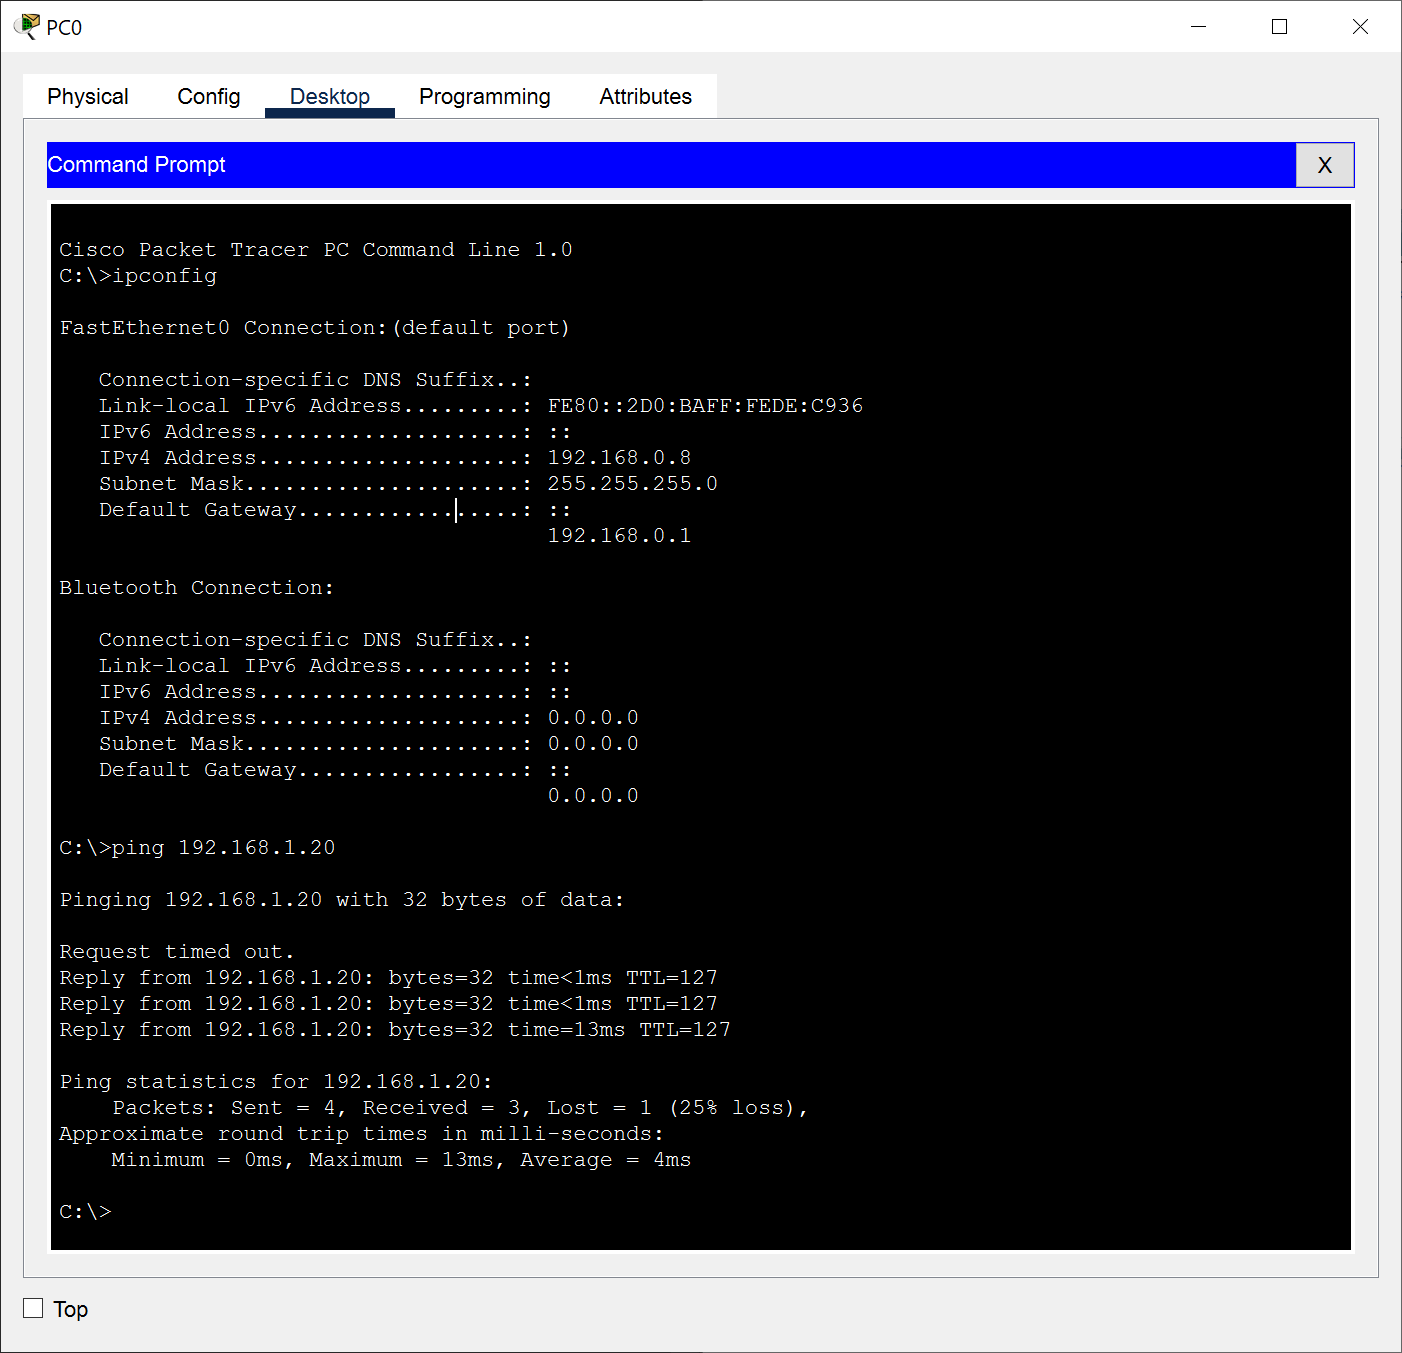
\includegraphics[width=13cm]{./step-by-step/21.PNG} \newline
\noindent We can safely assume the network is working
\clearpage



\section{Power over Ethernet}
Power over Ethernet is a technique for delivering DC power to devices over copper Ethernet cabling, eliminating the need for separate power supplies and outlets. While PoE doesn't add Ethernet data capabilities, it does offer expanded options for how and where Ethernet end devices can be placed.

%\section{LAN status LEDs}

\section{Network Topology}

Network topology is the arrangement of the elements (links, nodes, etc.) of a communication network.

Network topology is the structure of a network and may be depicted physically or logically. It is an application of graph theory wherein communicating devices are modeled as nodes and the connections between the devices are modeled as links or lines between the nodes. Physical topology is the placement of the various components of a network (e.g., device location and cable installation), while logical topology illustrates how data flows within a network. Distances between nodes, physical interconnections, transmission rates, or signal types may differ between two different networks, yet their logical topologies may be identical. A network’s physical topology is a particular concern of the physical layer of the OSI model.

Examples of network topologies are found in local area networks (LAN), a common computer network installation. Any given node in the LAN has one or more physical links to other devices in the network; graphically mapping these links results in a geometric shape that can be used to describe the physical topology of the network. A wide variety of physical topologies have been used in LANs, including ring, bus, mesh and star. Conversely, mapping the data flow between the components determines the logical topology of the network. In comparison, Controller Area Networks, common in vehicles, are primarily distributed control system networks of one or more controllers interconnected with sensors and actuators over, invariably, a physical bus topology.
\clearpage

\subsection{Star Topology}

In star topology, every peripheral node (computer workstation or any other peripheral) is connected to a central node called a hub or switch. The hub is the server and the peripherals are the clients. The network does not necessarily have to resemble a star to be classified as a star network, but all of the peripheral nodes on the network must be connected to one central hub. All traffic that traverses the network passes through the central hub, which acts as a signal repeater.

\noindent 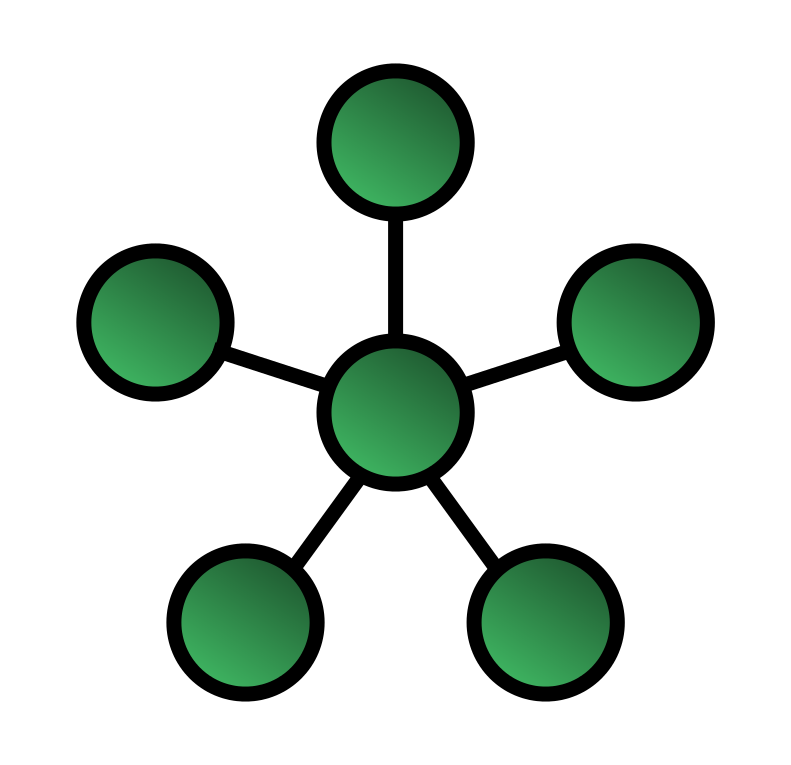
\includegraphics[width=7cm]{./StarNetwork.svg.PNG} \newline

\subsubsection{PROs}

\begin{itemize}
\item {simplicity of adding additional nodes}
\item {is the easiest topology to design and implement}
\end{itemize}

\subsubsection{CONs}

\begin{itemize}
\item {the hub represents a single point of failure}
\item {Since all peripheral communication must flow through the central hub, the aggregate central bandwidth forms a network bottleneck for large clusters}
\end{itemize}

\clearpage

\subsection{Ring Topology}

A ring topology is a daisy chain in a closed loop. Data travels around the ring in one direction. When one node sends data to another, the data passes through each intermediate node on the ring until it reaches its destination. The intermediate nodes repeat (re transmit) the data to keep the signal strong.\footnotemark{} Every node is a peer; there is no hierarchical relationship of clients and servers. If one node is unable to re transmit data, it severs communication between the nodes before and after it in the bus.

\noindent 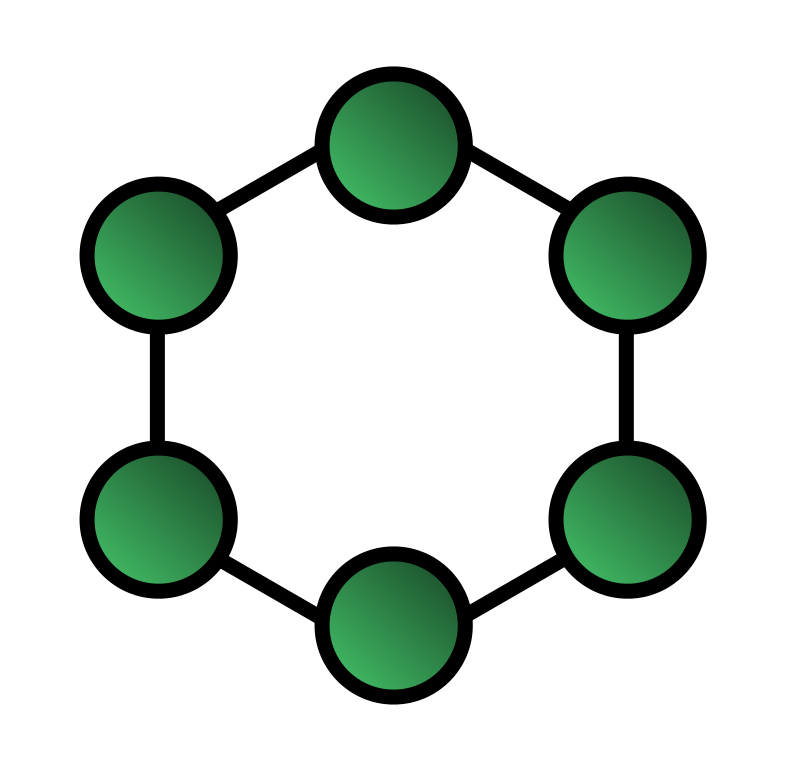
\includegraphics[width=7cm]{./RingNetwork.svg.PNG} \newline
\footnotetext{ Inc, S., (2002) . Networking Complete. Third Edition. San Francisco: Sybex }

\subsubsection{PROs}

\begin{itemize}
\item {When the load on the network increases, its performance is better than bus topology}
\item {There is no need of network server to control the connectivity between workstations}
\end{itemize}

\subsubsection{CONs}

\begin{itemize}
\item {Aggregate network bandwidth is bottlenecked by the weakest link between two nodes}
\end{itemize}

\clearpage
\subsection{Ring Topology on Cisco Packet Tracer}

This is a quick example of how can a Ring Topology look like on Cisco Packet Tracer. The links at the center have been added later on for testing purporses

\noindent 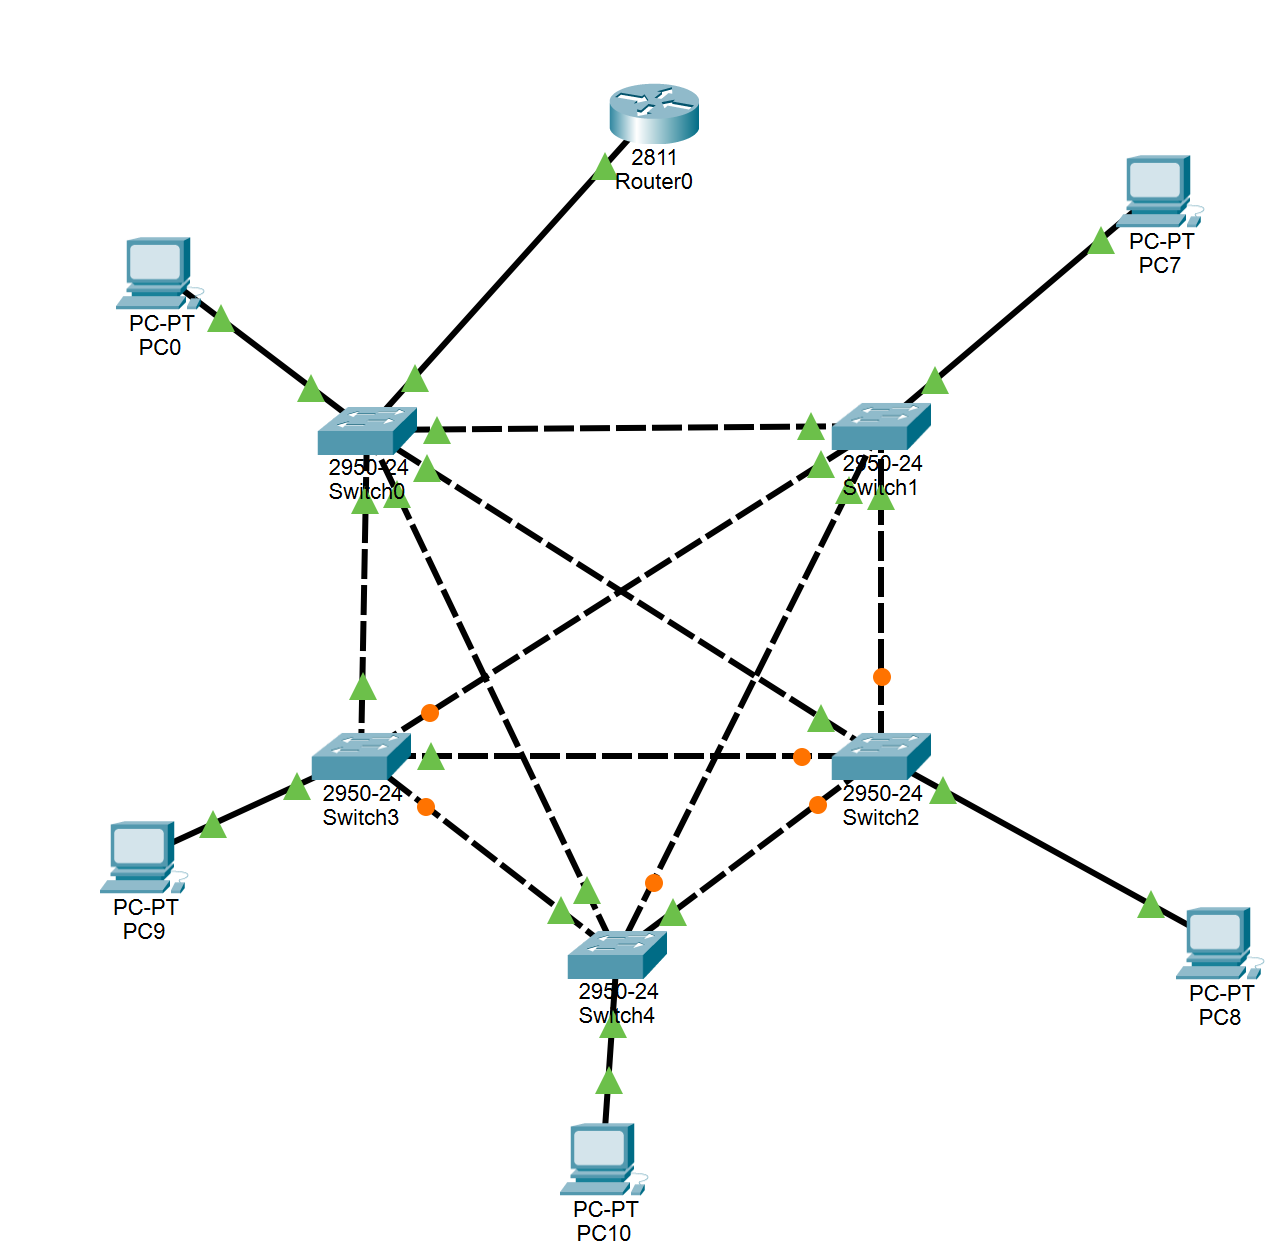
\includegraphics[width=7cm]{./star-topology/screenshot.PNG} \newline

\section{Routing Protocols}

A routing protocol specifies how routers communicate with each other to distribute information that enables them to select routes between nodes on a computer network. Routers perform the traffic directing functions on the Internet; data packets are forwarded through the networks of the internet from router to router until they reach their destination computer. Routing algorithms determine the specific choice of route. Each router has a prior knowledge only of networks attached to it directly. A routing protocol shares this information first among immediate neighbors, and then throughout the network. This way, routers gain knowledge of the topology of the network. The ability of routing protocols to dynamically adjust to changing conditions such as disabled connections and components and route data around obstructions is what gives the Internet its fault tolerance and high availability. \newline

The specific characteristics of routing protocols include the manner in which they avoid routing loops, the manner in which they select preferred routes, using information about hop costs, the time they require to reach routing convergence, their scalability, and other factors such as relay multiplexing and cloud access framework parameters. Certain additional characteristics such as multilayer interfacing may also be employed as a means of distributing uncompromised networking gateways to authorized ports. This has the added benefit of preventing issues with routing protocol loops.

Many routing protocols are defined in technical standards documents called RFCs

\section{Interior gateway protocols}
An interior gateway protocol (IGP) is a type of routing protocol used for exchanging routing table information between gateways (commonly routers) within an autonomous system (for example, a system of corporate local area networks). This routing information can then be used to route network-layer protocols like IP.

Interior gateway protocols can be divided into two categories: \textbf{distance-vector} routing protocols and \textbf{link-state} routing protocols.

\subsection{link state routing protocols}
Link-state routing protocols are one of the two main classes of routing protocols used in packet switching networks for computer communications, the other being distance-vector routing protocols. Examples of link-state routing protocols include Open Shortest Path First (OSPF) and Intermediate System to Intermediate System (IS-IS).

The link-state protocol is performed by every switching node in the network (i.e., nodes that are prepared to forward packets; in the Internet, these are called routers). The basic concept of link-state routing is that every node constructs a map of the connectivity to the network, in the form of a graph, showing which nodes are connected to which other nodes. Each node then independently calculates the next best logical path from it to every possible destination in the network. Each collection of best paths will then form each node's routing table.

This contrasts with distance-vector routing protocols, which work by having each node share its routing table with its neighbours, in a link-state protocol the only information passed between nodes is connectivity related. Link-state algorithms are sometimes characterized informally as each router, "telling the world about its neighbors."

\subsubsection{OSPF}
Open Shortest Path First (OSPF) is a routing protocol for Internet Protocol (IP) networks. It uses a link state routing (LSR) algorithm and falls into the group of interior gateway protocols (IGPs), operating within a single autonomous system (AS).

OSPF gathers link state information from available routers and constructs a topology map of the network. The topology is presented as a routing table to the Internet Layer for routing packets by their destination IP address. OSPF supports Internet Protocol Version 4 (IPv4) and Internet Protocol Version 6 (IPv6) networks and supports the Classless Inter-Domain Routing (CIDR) addressing model.

OSPF is widely used in large enterprise networks. IS-IS, another LSR-based protocol, is more common in large service provider networks.

Originally designed in the 1980s, OSPF is defined for IPv4 in protocol version 2 by RFC 2328 (1998).[1] The updates for IPv6 are specified as OSPF Version 3 in RFC 5340 (2008).[2] OSPF supports the Classless Inter-Domain Routing (CIDR) addressing model.

\subsection{distance vector routing protocols}
A distance-vector routing protocol in data networks determines the best route for data packets based on distance. Distance-vector routing protocols measure the distance by the number of routers a packet has to pass; one router counts as one hop. Some distance-vector protocols also take into account network latency and other factors that influence traffic on a given route. To determine the best route across a network, routers using a distance-vector protocol exchange information with one another, usually routing tables plus hop counts for destination networks and possibly other traffic information. Distance-vector routing protocols also require that a router inform its neighbours of network topology changes periodically.

Distance-vector routing protocols use the Bellman–Ford algorithm to calculate the best route. Another way of calculating the best route across a network is based on link cost, and is implemented through link-state routing protocols.

The term distance vector refers to the fact that the protocol manipulates vectors (arrays) of distances to other nodes in the network. The distance vector algorithm was the original ARPANET routing algorithm and was implemented more widely in local area networks with the Routing Information Protocol (RIP).

\subsubsection{RIP}
The Routing Information Protocol (RIP) is one of the oldest distance-vector routing protocols which employs the hop count as a routing metric. RIP prevents routing loops by implementing a limit on the number of hops allowed in a path from source to destination. The largest number of hops allowed for RIP is 15, which limits the size of networks that RIP can support.

RIP implements the split horizon, route poisoning, and holddown mechanisms to prevent incorrect routing information from being propagated.

In RIPv1 routers broadcast updates with their routing table every 30 seconds. In the early deployments, routing tables were small enough that the traffic was not significant. As networks grew in size, however, it became evident there could be a massive traffic burst every 30 seconds, even if the routers had been initialized at random times.

In most networking environments, RIP is not the preferred choice of routing protocol, as its time to converge and scalability are poor compared to EIGRP, OSPF, or IS-IS. However, it is easy to configure, because RIP does not require any parameters, unlike other protocols.

RIP uses the User Datagram Protocol (UDP) as its transport protocol, and is assigned the reserved port number 520.

\subsubsection{EIGRP}
Enhanced Interior Gateway Routing Protocol (EIGRP) is an advanced distance-vector routing protocol that is used on a computer network for automating routing decisions and configuration. The protocol was designed by Cisco Systems as a proprietary protocol, available only on Cisco routers. Functionality of EIGRP was converted to an open standard in 2013 and was published with informational status as RFC 7868 in 2016.

EIGRP is used on a router to share routes with other routers within the same autonomous system. Unlike other well known routing protocols, such as RIP, EIGRP only sends incremental updates, reducing the workload on the router and the amount of data that needs to be transmitted.

EIGRP replaced the Interior Gateway Routing Protocol (IGRP) in 1993. One of the major reasons for this was the change to classless IPv4 addresses in the Internet Protocol, which IGRP could not support.

\section{Exterior gateway protocols}

An exterior gateway protocol is a routing protocol used to exchange routing information between autonomous systems. This exchange is crucial for communications across the Internet. Notable exterior gateway protocols include Exterior Gateway Protocol (EGP), now obsolete, and Border Gateway Protocol (BGP)\footnote{\label{EGP}  Hunt, Craig (2002). \href{http://web.deu.edu.tr/doc/oreily/networking/tcpip/index.htm}{TCP/IP network administration} (3 ed.). O'Reilly Media. ISBN 9781449391430. OCLC 52356435. Archived from the original on 1 July 2020. Retrieved 5 November 2021 – via Dokuz Eylül University.}${}^{{}^{7 \cdot 5}}$:  

\subsection{BGP}
Border Gateway Protocol (BGP) is a standardized exterior gateway protocol designed to exchange routing and reachability information among autonomous systems (AS) on the Internet. BGP is classified as a path-vector routing protocol, and it makes routing decisions based on paths, network policies, or rule-sets configured by a network administrator.

BGP used for routing within an autonomous system is called Interior Border Gateway Protocol, Internal BGP (iBGP). In contrast, the Internet application of the protocol is called Exterior Border Gateway Protocol, External BGP (eBGP).

\section{IoT}
The \textbf{Internet of things} describes physical objects with sensors, processing ability, software, and other technologies that connect and exchange data with other devices and systems over the Internet or other communications networks.Internet of things has been considered a misnomer because devices do not need to be connected to the public internet, they only need to be connected to a network and be individually addressable.

\section{IoT in Aviation}
With the inclusion of digital technologies, the airline industry has now been able to deliver unique customer experiences, simplified underlying processes, and most importantly enhancing the productivity of the workforce. The next stride in leveraging IoT can lead to the exploration of newer dimensions in the aviation industry. Combining IoT with other technologies like AI and robotics would generate a number of opportunities related to service delivery improvement. Further, a smart  IoT ecosystem can bring in all the required entities and assets together in the industry value chain and make it look like the new normal.

\subsection{Existing Technologies in Aviation Industry}
\subsubsection{Digitized Security}
Today, state-of-the-art technology is being developed for implementing advanced concepts such as “walk through security” to reduce the passenger waiting times. Biometrics are also being used for automating the verification processes, thus reducing the burden of staffing.

Security systems are increasingly becoming a major technology trend at the airport terminals as these are equipped with the latest security system for security purposes.

\subsubsection{VR for Last-Minute Changes}
A leading global aviation company has been testing a new way for its passengers to upgrade their tickets by allowing them premium seats using VR. The airline company allows passengers to upgrade at the last  minute. The airline company said that the best way for understanding the benefits of a premium economy, that has extra legroom and seat pitch can be done virtualized using VR.

\subsubsection{Biometrics}
Biometrics are being potentially used by the aviation industry for some time now and is gaining a stronghold across this industry vertical. Some of the biggest airports across the world have invested in fingerprint and facial recognition technology. The aviation industry emphasizes on using facial recognition so that the passenger’s face becomes the new passport. Also at various airports, biometric-based recognition is being implemented at the airport lounge entrance and integrating this technology with flight information display systems for serving the passengers with a higher degree of personalized information along with offers.

\subsection{IoT Adoption Challenges}

\textbf{Following are some key challenges that are to be addressed for implementing IoT on a wide scale. These are inclusive of -}

\begin{itemize}
\item{ Most of the airline companies operate on a global level spread across diversified geographical boundaries. Each of these geographies has its own cultural diversity as well as technological adaptability. A successfully implemented IoT needs to support these regional variations.}
\item{ The airline industry operates in a top-notched secure environment. Thus, security and privacy need to be the top priority for implementing IoT in the aviation industry. Privacy can also be seen as a critical issue whenever there is a deployment of advanced technologies such as facial recognition as an outcome of the large volume of passenger’s private data.}
\end{itemize}

\subsection{Opportunities for IoT in Aviation}

IoT offers a number of tremendous benefits to the aviation industry and its rippling effects include- reduced travel times, enhancing the comfort levels of passengers with better security levels. In order to fully realize the \textbf{IoT} opportunities, the businesses and governments need to coordinate with the same frequency for answering the political as well as business issues related to IoT.

\noindent \textbf{This disruptive technology holds several benefits when it comes to the aviation industry -}

\begin{itemize}
\item{ When sensors are embedded in connected objects, it can be used for controlling, monitoring and collecting accurate real-time data. Sensors have significantly improved over the past few years. Wireless can be a key driver behind the emergence of IoT devices that operate on Wi-Fi or a strong cellular network such as 5G. Using a low-power wide area network (LPWAN) could be used for enriching the performance of sensors that offer low bandwidth.}
\item{ Cloud Computing can be used for creating a common platform for handling and integrating data from several sources like- people, their processes and their systems (devices). Real-time data can be utilized for gaining purposeful insights from current market data ad then distribute this information to the customers in a very short span of time.}
\item{ The airport terminals can duplicate the underlying concept of \textbf{smart cities}, thereby, implementing advanced technologies besides improved methods for collecting data to mine out the meaningful real-time insights. The use of sensor data could be done for improving operations and cumulative passenger experience. Multiple data sets can be integrated, optimized and analyzed for developing smarter applications and services related to airports, aircraft, and passengers.}
\item{ Beacons offer tremendous scope for IoT gateways. These can be placed across the entire airport infrastructure for triggering notifications on the passenger’s mobile as soon as he is in the beacon’s range. These notifications could be related to time, flight status or even displaying an e-boarding pass on the passenger’s mobile. This, in turn, provides the passenger with more accurate information every time. This can even help the airline crew for determining how far is the passenger from the airline in order to determine how long they need to wait before the actual take-off.}
\end{itemize}

\section{IPv6}

Internet Protocol version 6 (IPv6) is the most recent version of the Internet Protocol (IP), the communications protocol that provides an identification and location system for computers on networks and routes traffic across the Internet. IPv6 was developed by the Internet Engineering Task Force (IETF) to deal with the long-anticipated problem of IPv4 address exhaustion, and is intended to replace IPv4\footnotemark{}.

\begin{wrapfigure}{3cm}
\centering
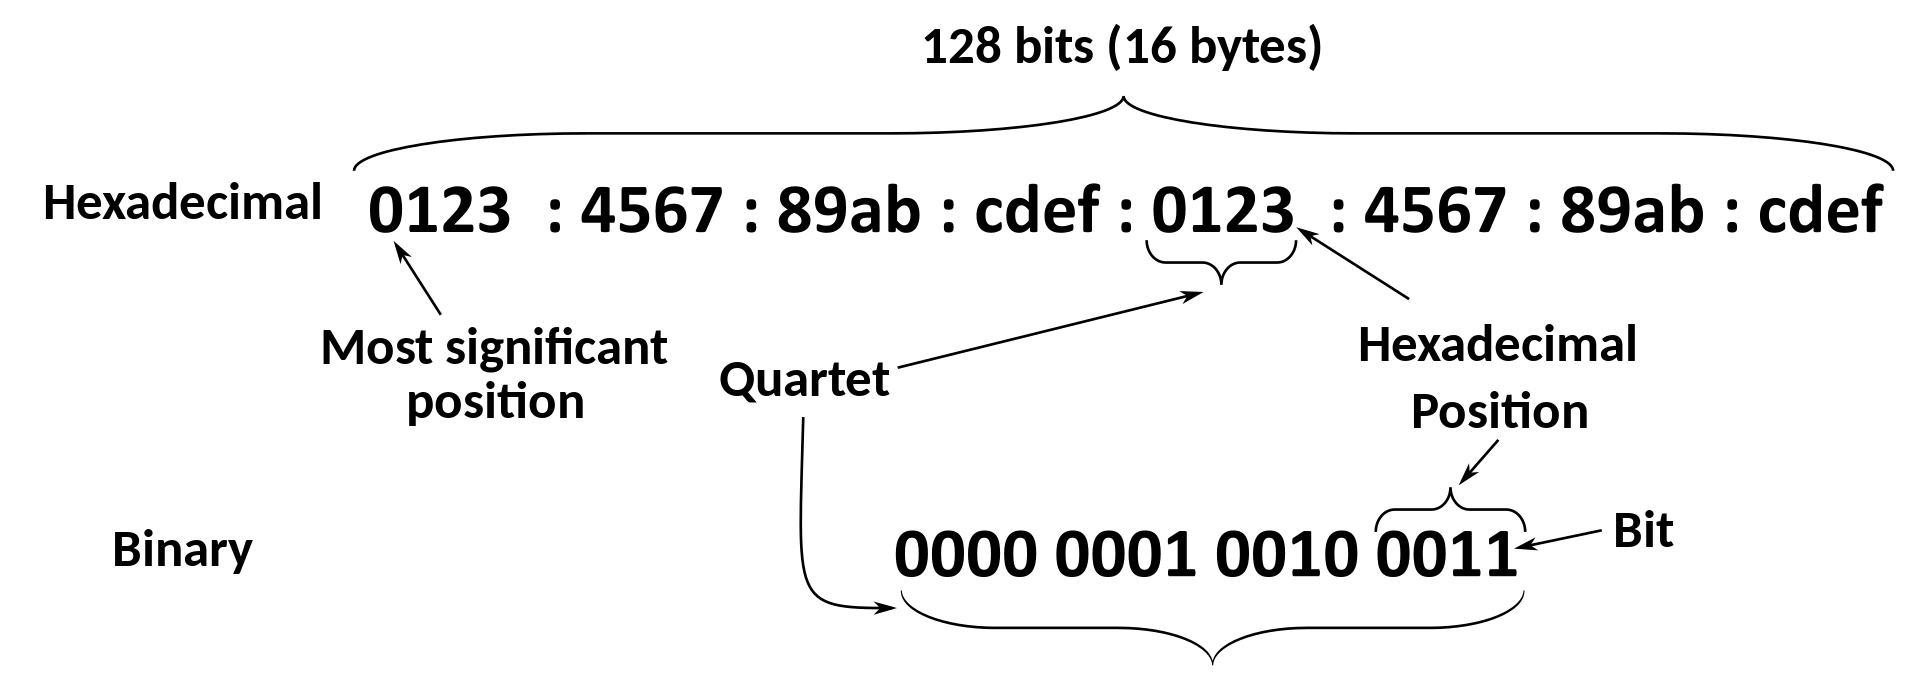
\includegraphics[width=10cm]{./IPv6.PNG}
%\vspace{-10pt}
\caption{IPv6 8-bytes Format }\label{wrap-fig:7}
\end{wrapfigure}

\footnotetext{ "FAQs". New Zealand IPv6 Task Force. Archived from the original on 29 January 2019. Retrieved 26 October 2015.}

\subsection{IPsec}
Internet Protocol Security (IPsec) was originally developed for IPv6, but found widespread deployment first in IPv4, for which it was re-engineered. IPsec was a mandatory part of all IPv6 protocol implementations,\footnote{\label{note1}\href{https://en.wikipedia.org/wiki/Steve_Deering}{S. Deering}; R. Hinden (December 1998), Internet Protocol, Version 6 (IPv6) Specification, \href{https://en.wikipedia.org/wiki/Internet_Engineering_Task_Force}{Internet Engineering Task Force} (IETF), RFC 2} and Internet Key Exchange (IKE) was recommended, but with RFC 6434 the inclusion of IPsec in IPv6 implementations was downgraded to a recommendation because it was considered impractical to require full IPsec implementation for all types of devices that may use IPv6.

However, as of RFC 4301 IPv6 protocol implementations that do implement IPsec need to implement IKEv2 and need to support a minimum set of cryptographic algorithms. This requirement will help to make IPsec implementations more interoperable between devices from different vendors. The IPsec Authentication Header (AH) and the Encapsulating Security Payload header (ESP) are implemented as IPv6 extension headers.\footnotemark{}


\footnotetext{ Silvia Hagen (2014). IPv6 Essentials: Integrating IPv6 into Your IPv4 Network (3rd ed.). Sebastopol, CA: O'Reilly Media. p. 196. ISBN 978-1-4493-3526-7. OCLC 881832733.}

\subsection{Link-local address}
In computer networking, a \textbf{link-local} address is a network address that is valid only for communications within the network segment or the broadcast domain that the host is connected to. Link-local addresses are most often assigned automatically with a process known as \textbf{stateless address autoconfiguration} or \textbf{link-local address autoconfiguration},\footnote{\label{autoconfiguration}S. Cheshire; B. Aboba; E. Guttma (May 2005). \href{https://datatracker.ietf.org/doc/html/rfc3927}{Dynamic Configuration of IPv4 Link-Local Addresses}. The Internet Society. doi:10.17487/RFC3927. RFC 3927. } also known as automatic private IP addressing (APIPA) or auto-IP.

\begin{wrapfigure}{3cm}
\centering
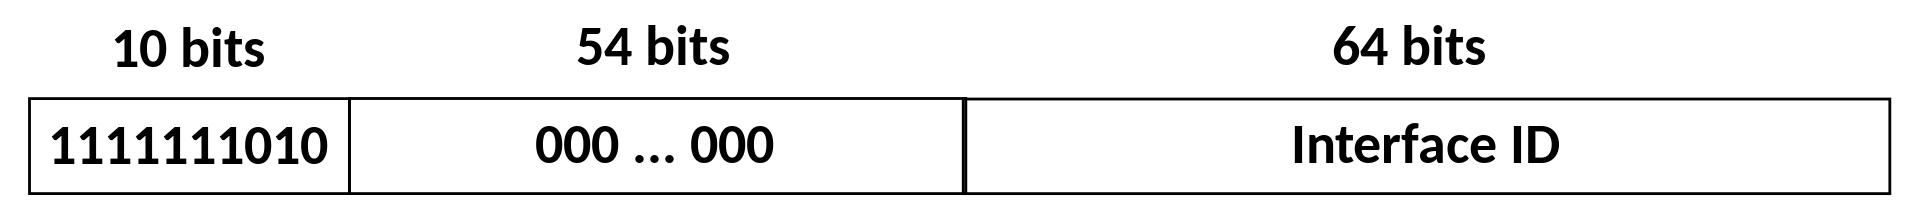
\includegraphics[width=10cm]{./IPv6_link_local_unicast_address_structure-en.svg.PNG}
%\vspace{-10pt}
\caption{IPv6 8-bytes Format }\label{wrap-fig:8}
\end{wrapfigure}


In the Internet Protocol Version 6 (IPv6), the address block fe80::/10 has been reserved for link-local unicast addressing.\footnote{\label{linklokal} R. Hinden; \href{https://en.wikipedia.org/wiki/Steve_Deering}{S. Deering} (February 2006). \href{https://datatracker.ietf.org/doc/html/rfc4291}{IP Version 6 Addressing Architecture}. IETF. doi:10.17487/RFC4291. RFC 4291. Updated by RFC 5952, RFC 6052, RFC 7136, RFC 7346, RFC 7371, RFC 8064.}}${}^{{}^{2 \cdot 4}}$ (IETF), RFC 2} Of the 64 bits of a link-local addresses' network component, the most significant 10 bits (1111111010) correspond to the IANA-reserved "global routing prefix" for link-local addresses, while the "subnet ID" (the remaining 54 bits) is zero$.^{\footnotemark[6 \ref{linklokal}^{2\cdot 5 \cdot}]}$ 

Unlike IPv4, IPv6 requires a link-local address on every network interface on which the IPv6 protocol is enabled, even when routable addresses are also assigned$.^{\footnotemark[8 \ref{linklokal}^{2\cdot}]}$ 

Consequently, IPv6 hosts usually have more than one IPv6 address assigned to each of their IPv6-enabled network interfaces. The link-local address is required for IPv6 sublayer operations of the Neighbor Discovery Protocol, as well as for some other IPv6-based protocols, such as DHCPv6.

When using an IPv6 link-local address to connect to a host, a zone index must be added to the address so that the packets can be sent out on the correct interface.

In IPv6, addresses may be assigned by stateless (automatic) or stateful (manual) mechanisms. Stateless address autoconfiguration is performed as a component of the Neighbor Discovery Protocol (NDP).\footnote{\label{NDP} S. Thomson; T. Narten; T. Jinmei (September 2007). \href{https://datatracker.ietf.org/doc/html/rfc4862}{IPv6 Stateless Address Autoconfiguration}. Network Working Group. doi:10.17487/RFC4862. RFC 4862. Obsoletes RFC 2462. Updated by RFC 7527.} The address is formed from its routing prefix and a unique identifier for the network interface.

Through NDP routing prefix advertisements, a router or server host may announce configuration information to all link-attached interfaces which causes additional IP address assignment on the receiving interfaces for local or global routing purposes. This process is sometimes also considered stateless, as the prefix server does not receive or log any individual assignments to hosts. Uniqueness is guaranteed automatically by the address selection methodology. It may be MAC-address based$,^{\footnotemark[1 \ref{NDP}]}$  or randomized.\footnote{\label{randomized} F. Gont; S. Krishnan; T. Narten; R. Draves (February 2021). \href{https://datatracker.ietf.org/doc/html/rfc8981}{Temporary Address Extensions for Stateless Address Autoconfiguration in IPv6}. IETF. doi:10.17487/RFC8981. ISSN 2070-1721. RFC 8981. Obsoletes RFC 4941.} Automatic duplicate address detection algorithms prevent assignment errors.



\section{IPv4}

Internet Protocol version 4 (IPv4) is the fourth version of the Internet Protocol (IP). It is one of the core protocols of standards-based internetworking methods in the Internet and other packet-switched networks.

\begin{wrapfigure}{3cm}
\centering
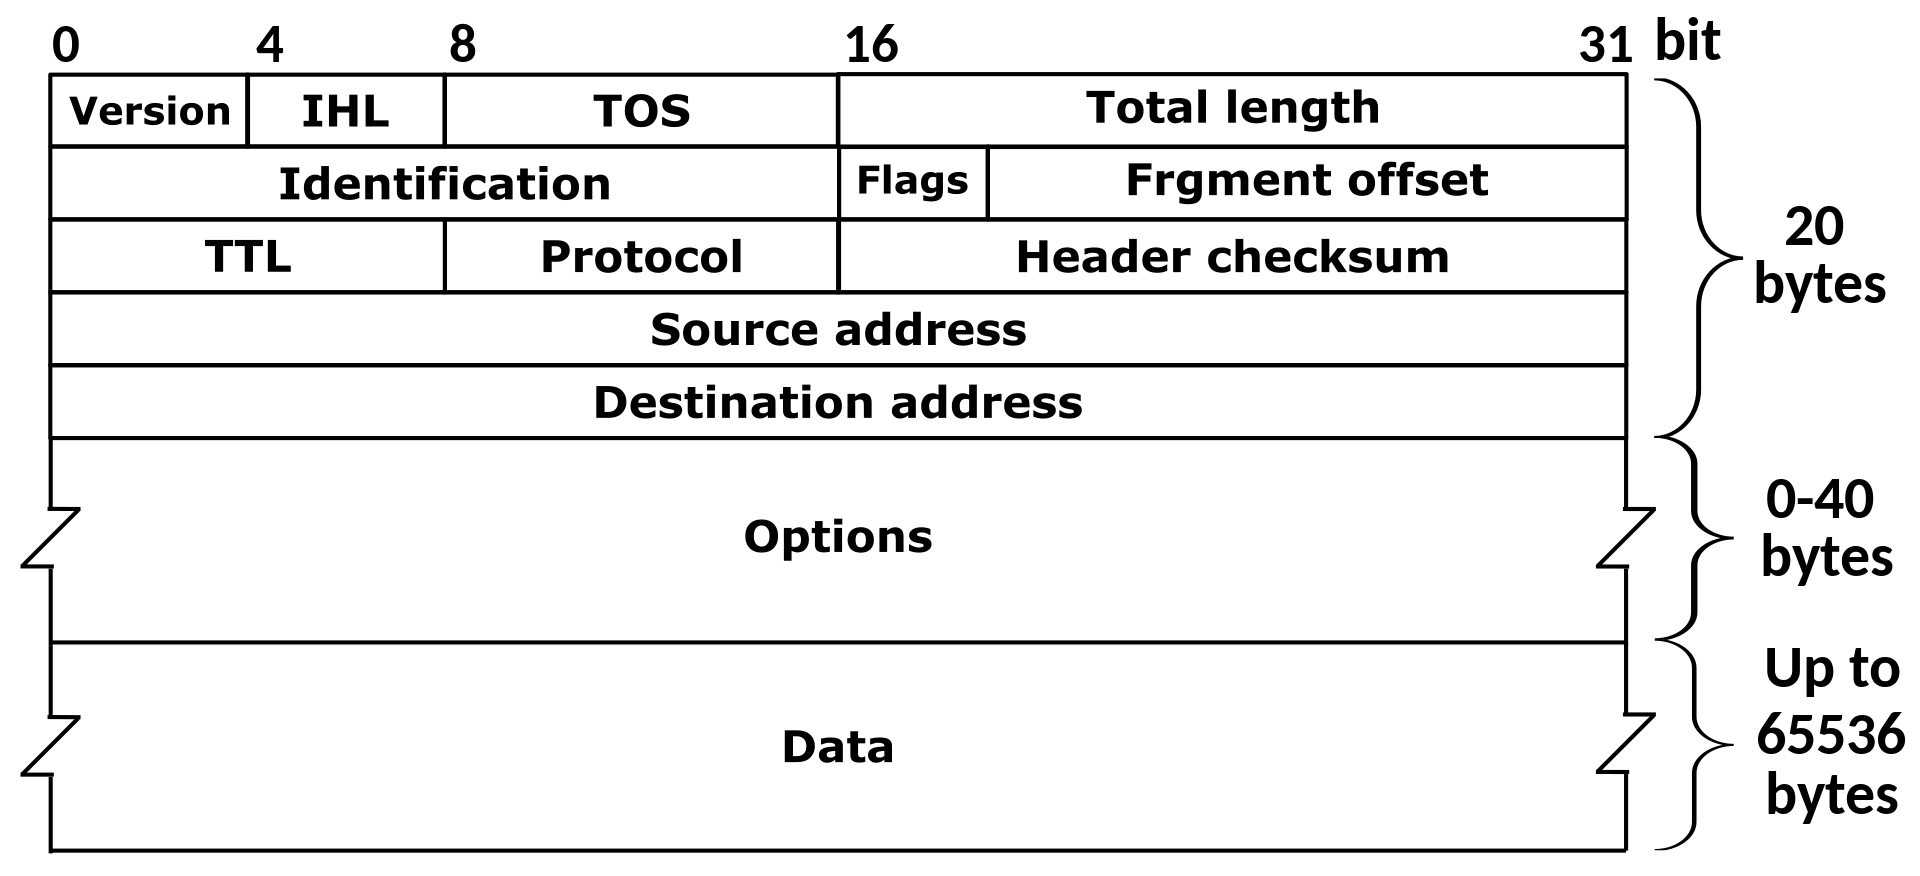
\includegraphics[width=10cm]{./IPv4_Packet-en.svg.PNG}
%\vspace{-10pt}
\caption{IPv6 8-bytes Format }\label{wrap-fig:9}
\end{wrapfigure}

IPv4 was the first version deployed for production on SATNET in 1982 and on the ARPANET in January 1983. It is still used to route most Internet traffic today,\footnote{\label{note2}\href{http://bgp.potaroo.net/index-bgp.html}{"BGP Analysis Reports"}. Retrieved 2013-01-09.} even with the ongoing deployment of Internet Protocol version 6 (IPv6),\footnote{\label{note3}\href{https://www.google.com/intl/en/ipv6/statistics.html}{"IPv6 – Google"}. www.google.com. Retrieved 2022-01-28.} its successor.

IPv4 uses a 32-bit address space which provides 4,294,967,296 ($2^{32}$) unique addresses, but large blocks are reserved for special networking purposes.\footnote{\label{note4}\href{https://www.iana.org/assignments/iana-ipv4-special-registry/iana-ipv4-special-registry.xhtml}{"IANA IPv4 Special-Purpose Address Registry"}. www.iana.org. Retrieved 2022-01-28.} \footnote{\label{note5}\href{https://datatracker.ietf.org/doc/html/rfc5735}{"RFC 5735 - Special Use IPv4 Addresses"}. datatracker.ietf.org. Retrieved 2022-01-28.}




\subsection{conversion to binary}

First a couple of words on the binary code first. A binary code is essentially text, computer processor low level instructions, or any other data using a two-symbol system. The two-symbol system used is often "0" and "1" from the \textbf{binary number system}. The binary code assigns a pattern of bits (aka binary digit), to each character, instruction, etc. For example, a binary string of eight bits can represent any of 256 possible values and can, therefore, represent a wide variety of different items.
In computing and telecommunications, binary codes are used for various methods of encoding data, such as character strings, into bit strings. 

Let's now convert 192.168.2.7 into binary
\newline

\begin{tabular}{||l|c|r|p{5cm}||}
    Division by 2 & Quotient & Remainder & Notes \\
    192/2 & 96 & 0 & This will be the 8th bit \\
    96/2 & 48 & 0 & The 7th bit \\
    48/2 & 24 & 0 & The 6th bit \\
    24/2 & 12 & 0 & The 5th bit \\
    12/2 & 6 & 0 & The 4th bit \\
    6/2 & 3 & 0 & The 3th bit \\
    3/2 & 1 & 1 & The 2nd bit \\
    1/2 & 0 & 1 & The 1st bit \\
\end{tabular}

\section{binary to Hex}

The hexadecimal system uses the number 16 as its base. As a $base^{16}$ numeral system, it uses 16 symbols. These are the 10 decimal digits 

\[0, 1, 2, 3, 4, 5, 6, 7, 8, 9\] and the first six letters of the English alphabet \[A, B, C, D, E, F\] which are representing the values 10, 11, 12, 13, 14 and 15.
This is useful in mathematics and IT as a more friendly way to represent binary. Each hex digit represents four binary digits; therefore you could say hex is a language to write binary in an abbreviated form.
Four binary digits make up half a byte. This means one byte can carry binary values from 0000 0000 to 1111 1111. In hex, these can be represented ranging from 00 to FF.
In html programming, colors can be represented by a 6-digit hexadecimal number: FFFFFF represents white whereas 000000 represents black.
Hex is more friendly in terms of possibility. It goes from 0 to 9 and then from A to F. It's 
The calculator has a \textbf{programmer} mode which allows you to use hex as well

\section{IP config}
Displays all current TCP/IP network configuration values and refreshes Dynamic Host Configuration Protocol (DHCP) and Domain Name System (DNS) settings. Used without parameters, ipconfig displays Internet Protocol version 4 (IPv4) and IPv6 addresses, subnet mask, and default gateway for all adapters.

\subsection{ipconfig/all}
Displays the full TCP/IP configuration for all adapters. Adapters can represent physical interfaces, such as installed network adapters, or logical interfaces, such as dial-up connections.

\subsection{ipconfig/displaydns}
Displays the contents of the DNS client resolver cache, which includes both entries preloaded from the local Hosts file and any recently obtained resource records for name queries resolved by the computer. The DNS Client service uses this information to resolve frequently queried names quickly, before querying its configured DNS servers.

The fields in the output of /displaydns correspond to the fields of an actual DNS reply.

\begin{itemize}
\item{In a DNS server's database, each piece of data is a "resource record".}
\item{"Record name" is the name you query DNS for, and the records (addresses or something else) belong to that name.}
\item{"Record type" is the type, displayed as a number - although more commonly they are referred to by their names, internally (in the DNS protocol) each has a number. Type 1 is "A" for "address", an IPv4 address. (IPv6 uses type 28, "AAAA", for an address four times as long.) "PTR", type 12, is a "pointer" to a hostname - most commonly used when mapping an IP address back to its name. "CNAME" is "canonical name".}
\item{"Time To Live" is the time in seconds after which the cache entry must expire.}
\item{"Data Length" appears to be the length in bytes - an IPv4 address is four bytes, IPv6 is sixteen bytes. For CNAME or PTR, Windows displays a static number (either 4 or 8, depending on your system) - this is actually the size of a memory address where the actual text is kept.}
\item{The "answer" section of a DNS reply is the actual answer to the query, and "additional" contains information that will likely be needed to find the actual answer. For example, glue records.}
\item{"<type> record" shows the actual value stored.}
\end{itemize}


\subsection{ipconfig/flushdns}
Flushes and resets the contents of the DNS client resolver cache. During DNS troubleshooting, you can use this procedure to discard negative cache entries from the cache, as well as any other entries that have been added dynamically.

\subsection{ipconfig/registerdns}
Initiates manual dynamic registration for the DNS names and IP addresses that are configured at a computer. You can use this parameter to troubleshoot a failed DNS name registration or resolve a dynamic update problem between a client and the DNS server without rebooting the client computer. The DNS settings in the advanced properties of the TCP/IP protocol determine which names are registered in DNS.

\subsection{ipconfig/flushdns-}

By default, most operating systems will cache IP addresses and other Domain Name System (DNS) records in order to fulfill future requests more quickly.

For example, when I type in https://lonezscents.com/ in my browser’s address bar for the first time, the browser has to ask DNS servers where to find the site. Once it has that information, the browser can store it in its local cache. Then, the next time I type in that website address, the browser will look for its DNS information in the local cache first and be able to find the site more quickly.

The problem is that sometimes dangerous IP addresses or corrupted results can be cached and need to be removed. The DNS cache can also impact your ability to connect to the internet or cause other issues. Whatever the reason, all major operating systems allow you to force the process of clearing this cache — or “flushing DNS.”

\subsubsection{what flush DNS does}
Flushing DNS will clear any IP addresses or other DNS records from your cache. This can help resolve security, internet connectivity, and other issues.

It’s important to understand that your DNS cache will clear itself out from time to time without your intervention. That’s because the DNS cache — in addition to saving all information that’s relevant to identifying and finding a website — also saves a component called TTL, or time to live. This specifies a period of time (in seconds) in which the DNS record for a site remains valid. Within this time period, any queries to the website are answered from the local cache without the help of the DNS server. Once the TTL expires, the entry will be removed from the cache.

However, there are reasons you may need to force a DNS flush rather than wait for the TTL of all the entries to expire. Let’s take a look at why below.

\subsubsection{why would you flush DNS}

There’s a few reasons you might need to flush your DNS cache. These reasons may have to do with security, technical problems, or data privacy. Let’s briefly cover each one below.

\begin{itemize}
\item{\textbf{You want to prevent DNS spoofing}.
DNS spoofing — also known as DNS cache poisoning — is an attack in which bad actors gain access to your DNS cache and alter the information in order to redirect you to the wrong sites. In some cases, they will redirect you to a fraudulent website that resembles its intended destination so that you enter in sensitive information, like your online banking login information.}

\item{\textbf{You’re seeing a 404 error}.
Let’s say you’ve cached the DNS information of a site that’s since moved to a new domain name or host. In that case, the DNS information on your computer may not get updated right away and you could end up seeing a 404 error or an outdated version of a site when you try to visit. Although the information will eventually get updated in your DNS cache, you don’t have to wait. You can clear DNS cache at any time.}

\item{\textbf{You’re having trouble accessing a website}.
If you’re having trouble getting a website to load, then you should try other steps first, like clearing your browser's temporary files and cookies and adjusting your browser settings to turn off pop-up blockers and allow sites to save and read cookies. But if you’ve exhausted your options, then you can flush DNS to reset your computer's connection to the internet.}

\item{\textbf{You want to keep your search behavior private}.
When you think of tracking user behavior on the internet, you probably think of cookies — but the DNS cache can reveal your search history as well. That’s because the DNS cache is designed to act like a virtual address book, storing the information of the websites you visit regularly. To keep this information away from data collectors or bad actors on the web, it’s a good idea to regularly flush your DNS cache.}
\end{itemize}
Now that we understand what flushing your DNS cache means and why you’d want to, let’s walk through how you can do it below.



\section{DHCP}

\subsection{IPCONFIG renew and release}
The host asks the router to drop the network configuration and make a new one

\subsection{BYOD}
Bring your own device

\subsection{vulnerabilities in LAN}
Poor configuration and Poor encryption

\subsubsection{Poor configuration}

\subsubsection{Poor encryption}


\subsection{Fixed IP}
So that someone doesn't just plug a device and gets an IP-address from DHCP. A device needs to be approved in order to receive an IP

\section{dns root server}
There are 13 important DNS root servers on the internet that store a complete database of domain names and their associated public IP addresses. These top-tier DNS servers are named A through M for the first 13 letters of the alphabet.Ten of these servers are in the US, one in London, one in Stockholm, and one in Japan 
\subsection{why 13 DNS servers}
That's exactly how much we need with IPv4. The IP packet size is 2 bytes.

\subsection{who manages}
The Internet Assigned Numbers Authority (IANA) keeps this list of DNS root servers if you're interested. ICANN manages them as well by delegating to IANA. It stands for Internet Corporation for Assigned Names and Numbers.

\section{The DNS Service}
The DNS service is the practical implementation of the DNS System. The DNS service is what a server running DNS software offers - the ability to use and manage DNS settings. Today, the DNS service is a very popular offer, with almost every domain registrar company offering their own DNS service. The DNS service can be run on a separate server, which is effective if running a very large and popular website, and can also be run on a shared hosting server, which is sufficient in 90\% of the cases.

\begin{itemize}
\item{recursive = non-authoritative}
\item{non-recursive = authoritative}
\end{itemize}

\section{The four DNS Servers to load a webpage}
Once a DNS query is entered, it passes through a few different servers before resolution, without any end-user interaction.

\subsection{DNS recursor}

This is a server designed specifically to receive queries from client machines. It tracks down the DNS record and makes additional requests to meet the DNS queries from the client. The number of requests can be decreased with DNS caching when the requested resources are returned to the recursor early on in the lookup process.

\subsection{Root name server}

This server does the job of translating the human-friendly hostnames into computer-friendly IP addresses. The root server accepts the recursor’s query and sends it to the TLD nameservers in the next stage, depending on the domain name seen in the query.

\subsection{dns server}

Top-Level Domain (TLD) nameserver

The TLD nameservers are responsible for maintaining the information about the domain names. For example, they could contain information about websites ending in “.com” or “.org” or country-level domains like “www.example.com.uk”, “www.example.com.us”, and others. The TLD nameserver will take the query from the root server and point it to the authoritative DNS nameserver associated with the query’s particular domain.

\subsection{Authoritative nameserver}

In the last step, the authoritative DNS nameserver will return the IP address back to the DNS recursor that can relay it to the client. This authoritative DNS nameserver is the one at the bottom of the lookup process that holds the DNS records. Think of these as the last stop or the final authoritative source of truth in the process.

\section{public dns}
public dns
\section{private dns}
private dns
\section{dns authentication}
dns authentication

\section{PING}
Ping is a computer network administration software utility used to test the reachability of a host on an Internet Protocol (IP) network. It is available for virtually all operating systems that have networking capability, including most embedded network administration software

Ping measures the round-trip time for messages sent from the originating host to a destination computer that are echoed back to the source. The name comes from active sonar terminology that sends a pulse of sound and listens for the echo to detect objects under water.[1]

Ping operates by means of Internet Control Message Protocol (ICMP) packets. Pinging involves sending an ICMP echo request to the target host and waiting for an ICMP echo reply. The program reports errors, packet loss, and a statistical summary of the results, typically including the minimum, maximum, the mean round-trip times, and standard deviation of the mean.

The command-line options of the ping utility and its output vary between the numerous implementations. Options may include the size of the payload, count of tests, limits for the number of network hops (TTL) that probes traverse, interval between the requests and time to wait for a response. Many systems provide a companion utility ping6, for testing on Internet Protocol version 6 (IPv6) networks, which implement ICMPv6.

\section{loopback}
Loopback (also written loop-back) is the routing of electronic signals or digital data streams back to their source without intentional processing or modification. It is primarily a means of testing the communications infrastructure.

There are many example applications. It may be a communication channel with only one communication endpoint. Any message transmitted by such a channel is immediately and only received by that same channel. In telecommunications, loopback devices perform transmission tests of access lines from the serving switching center, which usually does not require the assistance of personnel at the served terminal. Loop around is a method of testing between stations that are not necessarily adjacent, wherein two lines are used, with the test being done at one station and the two lines are interconnected at the distant station. A patch cable may also function as loopback, when applied manually or automatically, remotely or locally, facilitating a loop-back test.

Where a system (such as a modem) involves round-trip analog-to-digital processing, a distinction is made between analog loopback, where the analog signal is looped back directly, and digital loopback, where the signal is processed in the digital domain before being re-converted to an analog signal and returned to the source.

\section{subnet}
A subnetwork or subnet is a logical subdivision of an IP network.[1]: 1, 16  The practice of dividing a network into two or more networks is called subnetting.

Computers that belong to the same subnet are addressed with an identical most-significant bit-group in their IP addresses. This results in the logical division of an IP address into two fields: the network number or routing prefix and the rest field or host identifier. The rest field is an identifier for a specific host or network interface.

The routing prefix may be expressed in Classless Inter-Domain Routing (CIDR) notation written as the first address of a network, followed by a slash character (/), and ending with the bit-length of the prefix. For example, 198.51.100.0/24 is the prefix of the Internet Protocol version 4 network starting at the given address, having 24 bits allocated for the network prefix, and the remaining 8 bits reserved for host addressing. Addresses in the range 198.51.100.0 to 198.51.100.255 belong to this network, with 198.51.100.255 as the subnet broadcast address. The IPv6 address specification 2001:db8::/32 is a large address block with 296 addresses, having a 32-bit routing prefix.

For IPv4, a network may also be characterized by its subnet mask or netmask, which is the bitmask that, when applied by a bitwise AND operation to any IP address in the network, yields the routing prefix. Subnet masks are also expressed in dot-decimal notation like an IP address. For example, the prefix 198.51.100.0/24 would have the subnet mask 255.255.255.0.

Traffic is exchanged between subnetworks through routers when the routing prefixes of the source address and the destination address differ. A router serves as a logical or physical boundary between the subnets.

The benefits of subnetting an existing network vary with each deployment scenario. In the address allocation architecture of the Internet using CIDR and in large organizations, it is necessary to allocate address space efficiently. Subnetting may also enhance routing efficiency, or have advantages in network management when subnetworks are administratively controlled by different entities in a larger organization. Subnets may be arranged logically in a hierarchical architecture, partitioning an organization's network address space into a tree-like routing structure, or other structures such as meshes.

\section{Broadcast address}
A broadcast address is a network address used to transmit to all devices connected to a multiple-access communications network. A message sent to a broadcast address may be received by all network-attached hosts.

In contrast, a multicast address is used to address a specific group of devices, and a unicast address is used to address a single device.

For network layer communications, a broadcast address may be a specific IP address. At the data link layer on Ethernet networks, it is a specific MAC address
\subsection{single Broadcast address}
this is a consequence of having only one subnet, creating unnecessary traffic.

A task left is to create 2 subnets in the same local network
\subsection{vlans}
to make sure every subnet is isolated

\section{Multicast}
In computer networking, multicast is group communication[1] where data transmission is addressed to a group of destination computers simultaneously. Multicast can be one-to-many or many-to-many distribution.[2] Multicast should not be confused with physical layer point-to-multipoint communication.

Group communication may either be application layer multicast[1] or network-assisted multicast, where the latter makes it possible for the source to efficiently send to the group in a single transmission. Copies are automatically created in other network elements, such as routers, switches and cellular network base stations, but only to network segments that currently contain members of the group. Network assisted multicast may be implemented at the data link layer using one-to-many addressing and switching such as Ethernet multicast addressing, Asynchronous Transfer Mode (ATM), point-to-multipoint virtual circuits (P2MP)[3] or InfiniBand multicast. Network-assisted multicast may also be implemented at the Internet layer using IP multicast. In IP multicast the implementation of the multicast concept occurs at the IP routing level, where routers create optimal distribution paths for datagrams sent to a multicast destination address.

Multicast is often employed in Internet Protocol (IP) applications of streaming media, such as IPTV and multipoint videoconferencing.

\textbf{IGMP}

\section{Unicast}
In computer networking, unicast is a one-to-one transmission from one point in the network to another point; that is, one sender and one receiver, each identified by a network address.\footnote{\label{unicast}Godred Fairhurst \href{https://www.erg.abdn.ac.uk/users/gorry/course/intro-pages/uni-b-mcast.html}{"Unicast, Broadcast, and Multicast"}.}

Unicast is in contrast to multicast and broadcast which are one-to-many transmissions.

Internet Protocol unicast delivery methods such as Transmission Control Protocol (TCP) and User Datagram Protocol (UDP) are typically used.

\section{The Five IPv4 Classes}
In the IPv4 IP address space, there are five classes: A, B, C, D and E. Each class has a specific range of IP addresses (and ultimately dictates the number of devices you can have on your network). Primarily, class A, B, and C are used by the majority of devices on the Internet. Class D and class E are for special uses.

The list below shows the five available IP classes, along with the number of networks each can support and the maximum number of hosts (devices) that can be on each of those networks. The four octets that make up an IP address are conventionally represented by a.b.c.d - such as 127.10.20.30.

Additionally, information is also provided on private addresses and loop address (used for network troubleshooting).

\subsection{Class A Public & Private IP Address Range}
Class A addresses are for networks with large number of total hosts. Class A allows for 126 networks by using the first octet for the network ID. The first bit in this octet, is always zero. The remaining seven bits in this octet complete the network ID. The 24 bits in the remaining three octets represent the hosts ID and allows for approximately 17 million hosts per network. Class A network number values begin at 1 and end at 127.

\begin{itemize}
\item{Public IP Range: 1.0.0.0 to 127.0.0.0}
\item{First octet value range from 1 to 127}
\item{Private IP Range: 10.0.0.0 to 10.255.255.255}
\item{Subnet Mask: 255.0.0.0 (8 bits)}
\item{Number of Networks: 126}
\item{Number of Hosts per Network: 16,777,214}
\end{itemize}
 \clearpage
\subsection{Class B Public & Private IP Address Range}
Class B addresses are for medium to large sized networks. Class B allows for 16,384 networks by using the first two octets for the network ID. The first two bits in the first octet are always 1 0. The remaining six bits, together with the second octet, complete the network ID. The 16 bits in the third and fourth octet represent host ID and allows for approximately 65,000 hosts per network. Class B network number values begin at 128 and end at 191.

\begin{itemize}
\item{Public IP Range: 128.0.0.0 to 191.255.0.0}
\item{First octet value range from 128 to 191}
\item{Private IP Range: 172.16.0.0 to 172.31.255.255}
\item{Subnet Mask: 255.255.0.0 (16 bits)}
\item{Number of Networks: 16,382}
\item{Number of Hosts per Network: 65,534}
\end{itemize}

\subsection{Class C Public & Private IP Address Range}
Class C addresses are used in small local area networks (LANs). Class C allows for approximately 2 million networks by using the first three octets for the network ID. In a class C IP address, the first three bits of the first octet are always 1 1 0. And the remaining 21 bits of first three octets complete the network ID. The last octet (8 bits) represent the host ID and allows for 254 hosts per network. Class C network number values begins at 192 and end at 223.

\begin{itemize}
\item{Public IP Range: 192.0.0.0 to 223.255.255.0}
\item{First octet value range from 192 to 223}
\item{Private IP Range: 192.168.0.0 to 192.168.255.255}
\item{Special IP Range: 127.0.0.1 to 127.255.255.255}
\item{Subnet Mask: 255.255.255.0 (24 bits)}
\item{Number of Networks: 2,097,150}
\item{Number of Hosts per Network: 254}
\end{itemize}
\clearpage
\subsection{Class D IP Address Range}
Class D IP addresses are not allocated to hosts and are used for multicasting. Multicasting allows a single host to send a single stream of data to thousands of hosts across the Internet at the same time. It is often used for audio and video streaming, such as IP-based cable TV networks. Another example is the delivery of real-time stock market data from one source to many brokerage companies.

\begin{itemize}
\item{Range: 224.0.0.0 to 239.255.255.255}
\item{First octet value range from 224 to 239}
\item{Number of Networks: N/A}
\item{Number of Hosts per Network: Multicasting}
\end{itemize}


\subsection{Class E IP Address Class}
Class E IP addresses are not allocated to hosts and are not available for general use. These are reserved for research purposes.

\begin{itemize}
\item{Range: 240.0.0.0 to 255.255.255.255}
\item{First octet value range from 240 to 255}
\item{Number of Networks: N/A}
\item{Number of Hosts per Network: Research/Reserved/Experimental}
\end{itemize}

\clearpage
\printindex

\end{document}
